\documentclass[a4paper,11pt]{article}

% Encoding, Sprache, Typografie
\usepackage[utf8]{inputenc}
\usepackage[T1]{fontenc}
\usepackage[ngerman]{babel}
\usepackage{lmodern}
\usepackage{microtype}
\setlength{\emergencystretch}{2em}
\usepackage[a4paper,margin=2.5cm,headheight=14.5pt]{geometry}

\usepackage{amsmath, amssymb, amsthm, mathtools}
\numberwithin{equation}{subsection}
\usepackage{esvect}

% Grafiken und Tabellen
\usepackage{graphicx}
\usepackage{float}
\usepackage{caption}
\usepackage{subcaption}

\usepackage{booktabs}
\usepackage{colortbl}
\usepackage{pifont} % für einfache Symbol-Würfel (optional)

\usepackage{lipsum}

\usepackage{tikz}
\usepackage{tikz-dimline}
\usetikzlibrary{angles,quotes,arrows.meta,calc}
\usepackage{pgfplots}
\pgfplotsset{compat=1.18}
\usepgfplotslibrary{statistics} % stellt gausscdf bereit

\usepackage{fancyhdr}
\pagestyle{fancy} % Enable fancyhdr
\fancyhf{} % Clear all header/footer settings
\fancyhead[L]{\nouppercase{\leftmark}} % Left header: Chapter name
\fancyhead[R]{\thepage}
\fancyfoot[R]{\copyright\;Nils Schlager}
\fancyfoot[L]{\monthyeardate\today}
\renewcommand{\headrulewidth}{0.4pt} % Enable horizontal header line

% Kein Header wenn eine neue section beginnt
\usepackage{etoolbox}
\pretocmd{\section}{\thispagestyle{plain}}{}{}

% Listen, Farben, Links
\usepackage{enumitem}
\usepackage{xcolor}  
\definecolor{tocblue}{RGB}{0,92,170}  
\definecolor{accent}{RGB}{0,112,141}    % kühles Blaugrün
\definecolor{accent2}{RGB}{220,50,47}   % kräftiges Rot
\definecolor{accent3}{RGB}{46,139,87}   % kräftiges Grün (SeaGreen)
\definecolor{accent4}{RGB}{255,140,0}   % kräftiges Orange (DarkOrange)

\usepackage{hyperref}  
\hypersetup{  
  colorlinks=false,  
  pdfborder={0 0 0},
  linkcolor=tocblue,  
  urlcolor=tocblue,  
  citecolor=tocblue  
}
\usepackage{hypcap}

% ToC-Layout  
\usepackage{tocloft}  
  
% Füllpunkte (Leader) zwischen Eintrag und Seitenzahl  
\renewcommand{\cftdotsep}{2} % Abstand der Punkte (kleiner = dichter)  
\renewcommand{\cftsecleader}{\cftdotfill{\cftdotsep}}  
\renewcommand{\cftsubsecleader}{\cftdotfill{\cftdotsep}}

% Abschnittsebene fett im ToC  
\renewcommand{\cftsecfont}{\bfseries}  
\renewcommand{\cftsecpagefont}{\color{tocblue}\bfseries} % Seitenzahl rechts fett + blau

% Subsection normal (oder fett, wenn gewünscht)  
\renewcommand{\cftsubsecfont}{}  
\renewcommand{\cftsubsecpagefont}{\color{tocblue}}       % Seitenzahl rechts blau

\setlength{\cftbeforesecskip}{15pt}       % vertikaler Abstand zwischen Sections  
\setlength{\cftbeforesubsecskip}{5pt}    % vertikaler Abstand zwischen Subsections

\usepackage{titlesec}  
  
% Section: larger and bold  
\titleformat{\section}  
  {\bfseries\sffamily\huge}    % format for the whole title  
  {\thesection}                 % label  
  {0.8em}                       % spacing between label and title  
  {}                            % before-code  
  
% Subsection: a bit smaller than section  
\titleformat{\subsection}  
  {\bfseries\sffamily\LARGE}  
  {\thesubsection}  
  {0.6em}  
  {}

\usepackage[most]{tcolorbox}
\tcbset{  
  myleftbar/.style={  
    enhanced,  
    breakable,
    colback=white,  
    colframe=white,  
    borderline west={2pt}{0pt}{accent},  
    boxrule=0pt,  
    left=8pt,right=0pt,top=2pt,bottom=2pt,  
    sharp corners,  
  }  
}
% Zähler für Aufgaben/Lösungen: wird bei jeder Section zurückgesetzt  
\newcounter{aufg}[section]  
\renewcommand*\theaufg{\thesection.\arabic{aufg}}  
\newcounter{bsp}[section]  
\renewcommand*\thebsp{\thesection.\arabic{bsp}}  

% Titel-Makros verwenden automatisch die Nummer  
\newcommand{\bsptitel}{\textit{\textcolor{accent}{Beispiel~\thebsp.}}}  
\newcommand{\aufgabentitel}{\textit{\textcolor{accent}{Aufgabe~\theaufg.}}}  
\newcommand{\loesungstitel}{\textit{\textcolor{accent}{Lösung von Aufgabe~\theaufg.}}}  
  
% Umgebung für Aufgabe: erhöht Zähler  
\newenvironment{aufgabe}  
{%  
  \refstepcounter{aufg}% erhöht und macht referenzierbar  
  \begin{tcolorbox}[myleftbar]%  
  \aufgabentitel\ %  
}  
{%  
  \end{tcolorbox}
}  
% Umgebung für Lösung: gleiche Nummer wie vorherige Aufgabe  
\newenvironment{loesung}  
{%  
  \begin{tcolorbox}[myleftbar]%  
  \loesungstitel\ %  
}  
{%  
  \end{tcolorbox} \noindent
}
% Beispiel
\newenvironment{bsp}  
{%  
  \refstepcounter{bsp}%  
  \begin{tcolorbox}[myleftbar]%  
  \bsptitel\ %  
}  
{%  
  \end{tcolorbox}\vspace{6pt}  
}

% Geogebra
\lstdefinestyle{ggb}{
  basicstyle=\ttfamily\small,
  columns=fullflexible,
  tabsize=2,
  showstringspaces=false,
  breaklines=true,
  keywordstyle=\color{accent}\bfseries,
  commentstyle=\color{gray!70}\itshape,
  morekeywords={Löse, NLöse, Test},
  literate={ä}{{\"a}}1 {ö}{{\"o}}1 {ü}{{\"u}}1
           {Ä}{{\"A}}1 {Ö}{{\"O}}1 {Ü}{{\"U}}1 {ß}{{\ss}}1,
}

% Full bordered GeoGebra code box with logo in a titled chip at top-left
\newtcblisting{geogebracode}{  
  enhanced, breakable,  
  listing only,  
  listing engine=listings,  
  listing options={style=ggb},  
  colback=white,          % code background  
  colframe=accent,        % frame color  
  boxrule=0.9pt,  
  arc=2pt,                % rounded corners; set to 0pt if you want square  
  left=10pt, right=10pt, bottom=-5pt, top=14pt, % extra top padding for header row  
  overlay={  
    % Header row: logo + plain title text inside the box (no background or frame)  
    \node[anchor=north west] at ([xshift=0pt,yshift=0pt]frame.north west) {%  
      \raisebox{-0.25em}{
\includegraphics[height=1.2em]{Geogebra.svg.png}}\hspace{2pt}%  
      \textit{\textcolor{accent}{GeoGebra}}%  
    };  
  },  
}


% Display Dices in text
\newcommand{\dice}[1]{%  
  \tikz[baseline=-0.8ex]{  % <-- Anpassung für vertikale Zentrierung  
    \node[draw=accent, thick, minimum width=10pt, minimum height=10pt, inner sep=1pt, rounded corners=2pt] (die) {};  
    % Punkte je nach Zahl  
    \ifnum#1=1  
      \fill[accent] (0,0) circle (0.8pt);  
    \fi  
    \ifnum#1=2  
      \fill[accent] (-0.09,0.09) circle (0.8pt);  
      \fill[accent] (0.09,-0.09) circle (0.8pt);  
    \fi  
    \ifnum#1=3  
      \fill[accent] (-0.09,0.09) circle (0.8pt);  
      \fill[accent] (0,0) circle (0.8pt);  
      \fill[accent] (0.09,-0.09) circle (0.8pt);  
    \fi  
    \ifnum#1=4  
      \fill[accent] (-0.09,0.09) circle (0.8pt);  
      \fill[accent] (0.09,0.09) circle (0.8pt);  
      \fill[accent] (-0.09,-0.09) circle (0.8pt);  
      \fill[accent] (0.09,-0.09) circle (0.8pt);  
    \fi  
    \ifnum#1=5  
      \fill[accent] (-0.09,0.09) circle (0.8pt);  
      \fill[accent] (0.09,0.09) circle (0.8pt);  
      \fill[accent] (0,0) circle (0.8pt);  
      \fill[accent] (-0.09,-0.09) circle (0.8pt);  
      \fill[accent] (0.09,-0.09) circle (0.8pt);  
    \fi  
    \ifnum#1=6  
      \fill[accent] (-0.09,0.09) circle (0.8pt);  
      \fill[accent] (0,0.09) circle (0.8pt);  
      \fill[accent] (0.09,0.09) circle (0.8pt);  
      \fill[accent] (-0.09,-0.09) circle (0.8pt);  
      \fill[accent] (0,-0.09) circle (0.8pt);  
      \fill[accent] (0.09,-0.09) circle (0.8pt);
    \fi  
  }%  
}

% Display fat dot in text
\NewDocumentCommand{\fatdot}{O{black} O{3pt} O{-0.5ex}}{  
\mathord{  
  \tikz[baseline=#3]  
    \node[fill=#1, circle, inner sep=#2] {};  
    }  
}
% usage: \fatdot[red][5pt][0.5ex]

\usepackage{datetime}
\newdateformat{monthyeardate}{%
  \monthname[\THEMONTH], \THEYEAR}

% Titel
\title{\textbf{Skriptum: Mathematik-Matura}}
\author{Nils Schlager}
\date{\today}

\begin{document}
% Farben aus dem Bild definieren
\definecolor{coverblue}{RGB}{0,115,165}
\definecolor{covergray}{RGB}{58,58,60}
\thispagestyle{empty}

\begin{tikzpicture}[remember picture,overlay]
  % Vertikaler Text auf dem grauen Balken
    \node[rotate=90, anchor=south,
        font=\sffamily\bfseries\fontsize{54}{64}\selectfont,
        text=coverblue] % oder text=coverblue, wenn du das Blau als Schrift willst
    at ($(current page.west) + (3cm,0cm)$)
        {MATHEMATIK -- MATURA};

    \node[text=black, anchor=west, align=right]
    at ($(current page.north) - (4.5cm,7cm)$)
        { 
            \begin{tabular}{r}
                \Huge Skriptum zur AHS-Matura \\[0.5cm]
                \Large \today \\[0.5cm]
                \Large Nils Schlager
            \end{tabular}
        };


    \draw[rounded corners=10pt, coverblue,line width=6pt] 
    ($(1.5,-1)$) rectangle ($(3,-1)+(20,-6)$);    

    \node[text=black, anchor=west, align=right]
    at ($(current page.north) - (-5cm,28cm)$) {Version 1.0.0};
    

\def\xoffset{1}   % change this to shift everything in x
\def\yoffset{0}   % change this to shift everything in y

\node[opacity=0.5] at ($ (8,-16) + (\xoffset,\yoffset) $) 
  {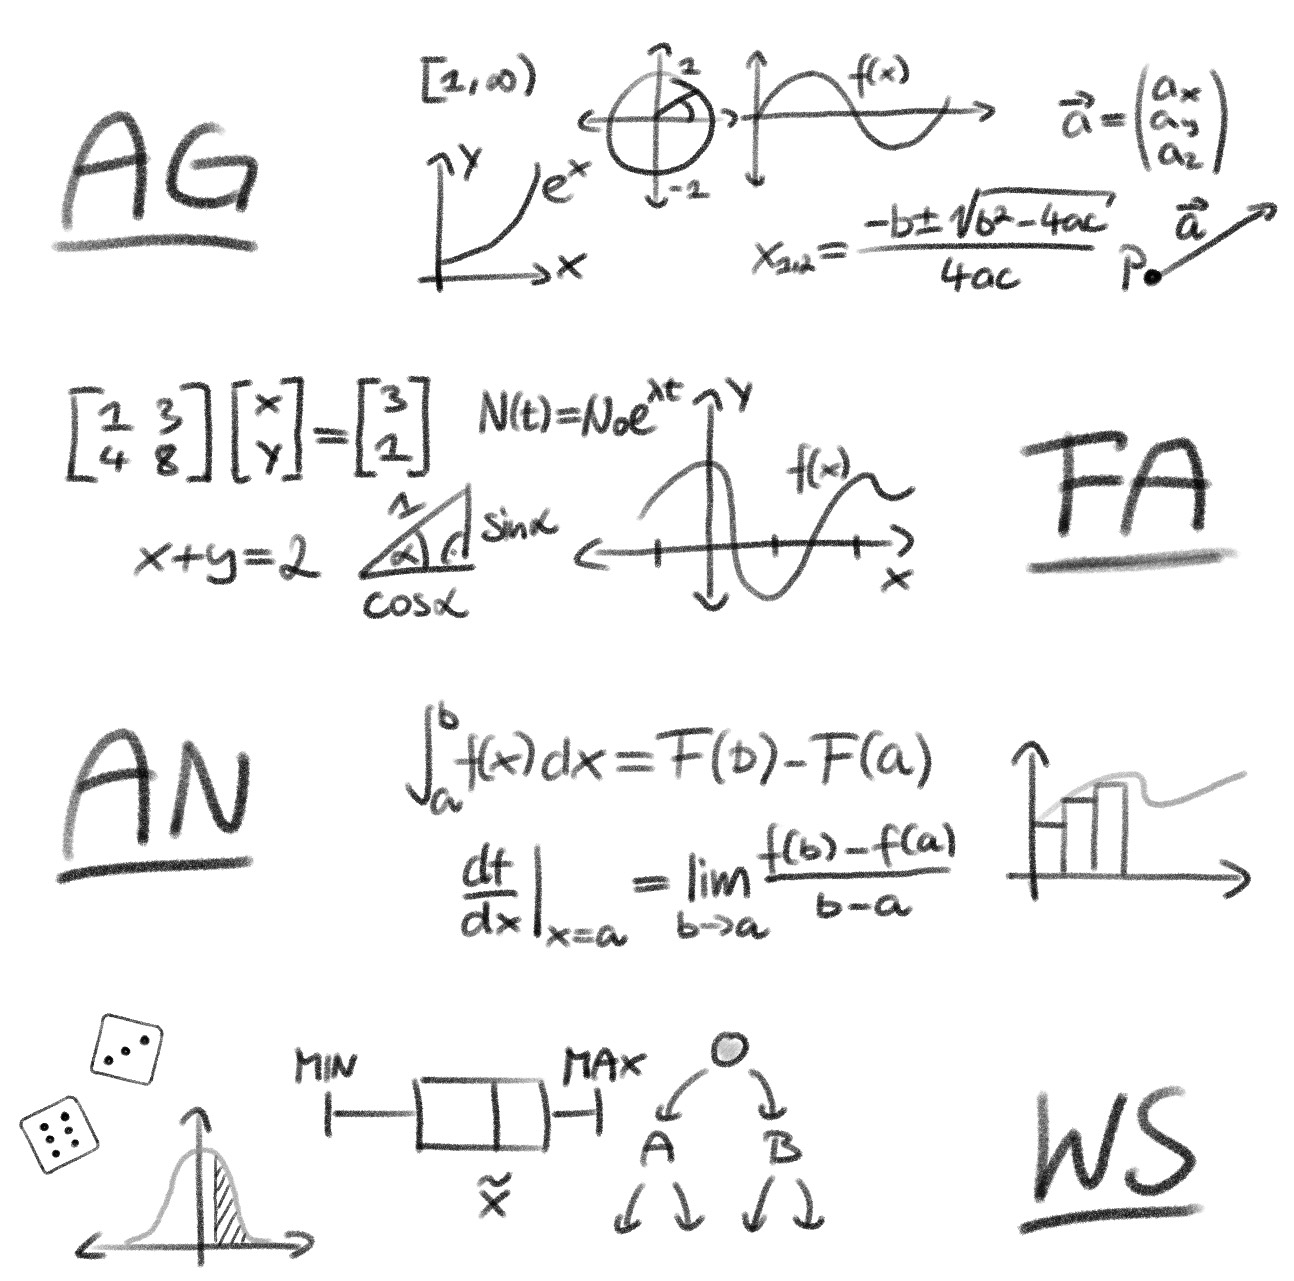
\includegraphics[width=14cm]{background.png}};

\draw[rounded corners=8pt] 
  ($ (1,-9.5) + (\xoffset,\yoffset) $) 
  rectangle 
  ($ (1,-9.5) + (3.5,-3) + (\xoffset,\yoffset) $);

\draw[rounded corners=8pt] 
  ($ (5,-9.5) + (\xoffset,\yoffset) $) 
  rectangle 
  ($ (5,-9.5) + (10,-3) + (\xoffset,\yoffset) $);

\draw[rounded corners=8pt] 
  ($ (11.5,-13) + (\xoffset,\yoffset) $) 
  rectangle 
  ($ (11.5,-13) + (3.5,-3) + (\xoffset,\yoffset) $);

\draw[rounded corners=8pt] 
  ($ (1,-13) + (\xoffset,\yoffset) $) 
  rectangle 
  ($ (1,-13) + (10,-3) + (\xoffset,\yoffset) $);

\draw[rounded corners=8pt] 
  ($ (1,-16.5) + (\xoffset,\yoffset) $) 
  rectangle 
  ($ (1,-16.5) + (3.5,-3) + (\xoffset,\yoffset) $);

\draw[rounded corners=8pt] 
  ($ (5,-16.5) + (\xoffset,\yoffset) $) 
  rectangle 
  ($ (5,-16.5) + (10,-3) + (\xoffset,\yoffset) $);

\draw[rounded corners=8pt] 
  ($ (11.5,-20) + (\xoffset,\yoffset) $) 
  rectangle 
  ($ (11.5,-20) + (3.5,-3) + (\xoffset,\yoffset) $);

\draw[rounded corners=8pt] 
  ($ (1,-20) + (\xoffset,\yoffset) $) 
  rectangle 
  ($ (1,-20) + (10,-3) + (\xoffset,\yoffset) $);
\end{tikzpicture}
\clearpage

\setcounter{tocdepth}{2}
\tableofcontents

\vfill
\subsubsection*{Hinweis}
Dieses Skript wurde im Rahmen zahlreicher Nachhilfestunden erstellt und orientiert sich an den Themenbereichen der Mathematik für die AHS-Matura. Es dient SchülerInnen als Nachschlagewerk und Verständnishilfe. Das Skript erhebt keinen Anspruch auf Vollständigkeit; vielmehr fasst es aus meiner Sicht die wichtigsten Inhalte kurz und übersichtlich zusammen.

\pagebreak
\section{Algebra \& Geometrie (AG)}
\subsection{Grundbegriffe der Algebra}
\subsubsection{Zahlenmengen}
\newcommand{\R}{\mathbb{R}}  
\newcommand{\N}{\mathbb{N}}  
\newcommand{\Q}{\mathbb{Q}}  
\newcommand{\Z}{\mathbb{Z}}  
\newcommand{\C}{\mathbb{C}}
\newcommand{\eps}{\varepsilon}
\newcommand{\veci}{\mathrm{i}} % imaginäre Einheit
Die \textbf{natürlichen Zahlen} sind definiert als
\[
    \N = \{1,2,3,4,\dots\}.
\]
und sind eine unbeschränkte Menge. Je nach Definition wird die Zahl 0 dazugenommen, wodurch man Folgendes erhält:
\[
    \N_0 = \{0,1,2,3,4,\dots\}
\]
Die \textbf{ganzen Zahlen} beinhalten die natürlichen Zahlen und die entsprechenden Gegenzahlen
\[
    \Z = \{\dots,-2,-1,0,1,2,\dots\}.
\]
\textbf{Rationale Zahlen} sind Zahlen die als Bruch ganzer Zahlen dargestellt werden können
\[
    \Q=\left\{\frac{p}{q}\,\middle|\, p,q\in\Z,\, q\neq 0\right\}.
\]
Man erhält die \textbf{reellen Zahlen} (\(\R\)), indem man die rationalen Zahlen und irrationalen Zahlen (Zahlen die nicht als Bruch ganzer Zahlen dargestellt werden können) vereint. \\[5pt]
Die \textbf{komplexen Zahlen} (\(\C\)) beihalten alle reellen Zahlen und werden über die imaginäre Einheit \(i=\sqrt{-1}\) dargestellt.
\[
z=a+b\veci,\quad a,b\in\R,\qquad \veci^2=-1.
\]
Dabei ist \(a\) Realteil und \(b\) Imaginärteil. \\[5pt]
Die Zahlenmengen sind folgendermaßen zueinander angeordnet (das Symbol \(\subset\) bedeutet Teilmenge):
\[
\N \subset \Z \subset \Q \subset \R \subset \C.
\]

\begin{center}
\begin{tikzpicture}[scale=.8, every node/.style={font=\large}]
  % Complex numbers (outermost)
  \draw[thick] (0,0) ellipse (5.5 and 2);
  \node at (4.7,0) {$\mathbb{C}$};

  % Real numbers
  \draw[thick] (-0.5,0) ellipse (4.5 and 1.7);
  \node at (3.25,0) {$\mathbb{R}$};

  % Rational numbers
  \draw[thick] (-1.0,0) ellipse (3.5 and 1.3);
  \node at (1.5,0) {$\mathbb{Q}$};

  % Integers
  \draw[thick] (-1.5,0) ellipse (2.4 and 0.9);
  \node at (0,0) {$\mathbb{Z}$};

  % Natural numbers
  \draw[thick] (-2.0,0) ellipse (1.3 and 0.5);
  \node at (-2,0) {$\mathbb{N}$};
\end{tikzpicture}
\captionof{figure}{Mengenbeziehungen der Zahlenmengen} 
\end{center}

\begin{bsp} Im Folgenden sind einige Zahlen für die jeweiligen Zahlenmengen angegeben \vspace{5pt}\\
rationale Zahlen: \(1,\,-2,\,\frac{4}{3}=1.\dot{3},\,\frac{5}{2}=2.5,\,\frac{1}{3}=0.\dot{3}\) \vspace{3pt}\\
irrationale Zahlen: \(\sqrt{2},\,\sqrt{3},\,e=2.71828...,\,\pi=3.1415...\) \vspace{3pt}\\
reelle Zahlen: \(-2,\,\frac{4}{3}=1.\dot{3},\,\frac{5}{2}=2.5,\,e,\,pi,\,\sqrt{3}\) \vspace{3pt}\\
komplexe Zahlen \(4+3\veci,\, 10\veci,\, 8-\veci\)
\end{bsp}

\subsubsection{Intervalle}
Abgeschlossene Intervalle werden mit eckigen Klammern geschrieben und beinhalten auch die beiden Randpunkte:
\begin{equation}
    [a,b] = \{x \in \R : a \leq x \leq b\}
\end{equation}
Bei offenen Intervallen werden runde Klammern verwendet. Die Randpunkte sind hier nicht enthalten:
\begin{equation}
    (a,b) = \{x \in \R : a < x < b\}
\end{equation}
Intervalle können auch auf einer Seite offen und auf der anderen Seite geschlossen sein. Kommt die Zahl $\infty$ vor so ist immer eine Klammer zu verwenden.
\begin{bsp}
    \begin{equation*}
        [5,\infty) = \{ x \in \R : x \geq 5 \}
    \end{equation*}
\end{bsp}
\subsubsection{Betrag einer Zahl}
Der Betrag einer Zahl (auch Absolutwert genannt) beschreibt, wie weit eine Zahl vom Nullpunkt entfernt ist (ohne Vorzeichen) und ist wie folgt definiert:
\begin{equation}
    |x| =
    \begin{cases}
        x, & \text{wenn } x \ge 0, \\
        -x, & \text{wenn } x < 0.
    \end{cases}
\end{equation}
Das bedeutet wenn \(x\) positiv oder 0 ist bleibt der Wert der Zahl gleich und wenn x negativ ist wird das Minuszeichen entfernt.

\subsection{(Un-)Gleichungen und Gleichungssysteme}
Verbindet man zwei Therme (linke und rechte Seite) durch ein Gleichheitszeichen, erhält man eine Gleichung. Diese Gleichung enthält eine Unbekannte, welche durch \textbf{Äquivalenzumformungen} berechnet werden kann. \\
Die \textbf{Grundmenge} \(G\) ist die Menge aller Zahlen, aus denen die Lösungen einer Gleichung stammen dürfen. Sie legt also fest, in welchem Zahlenbereich man arbeitet. \\
Die \textbf{Definitionsmenge} \(D\) umfasst die Zahlen die man in die Gleichung einsetzen darf:
\begin{itemize}
    \item keine Division durch 0
    \item keine Wurzeln aus negativen Zahlen
    \item kein Logarithmus von negativen Zahlen
\end{itemize}
Die \textbf{Lösungsmenge} \(L\) enthält alle Lösungen einer Gleichung und kann auch leer sein oder die ganze Definitionsmenge enthalten.
\begin{aufgabe}
    Gib die Defintionsmenge folgender Gleichungen an: \\
    \[
        \frac{1}{x}=2,\quad 2\cdot x+3=5,\quad \frac{5x-3}{x-1},\quad \sqrt{x+3}=5
    \]
\end{aufgabe}
\begin{loesung}
    \[
        D_1=\R \setminus \{0\}, \quad
        D_2=\R, \quad
        D_3=\R \setminus \{1\}, \quad
        D_4=[-3,\infty)
    \]
\end{loesung}
\subsubsection{Lineare Gleichungen}
Lineare Gleichungen sind Gleichungen in denen die Unbekannte nur in der ersten Potenz vorkommt:
\begin{equation}
    a \cdot x + b = 0,\quad a,b \in \R
\end{equation}
Ihre Lösung kann als Nullstelle der zugehörigen linearen Funktion \(f(x)=k\cdot x + d\) interpretiert werden.
\begin{aufgabe}
    Ermittle die Lösung folgender linearer Gleichung: \(2\cdot x - 3 = 0\)
\end{aufgabe}
\begin{loesung}
    \begin{align*}
        2\cdot x - 3 &= 0 \\
        2\cdot x &= 3 \\
        x &= \frac{3}{2} = 1.5
    \end{align*}
\end{loesung}
\begin{geogebracode}
Löse(2*x-3=0,x)   // Symbolische Lösung
NLöse(2*x-3=0,x)  // Numerische Lösung
\end{geogebracode}
\subsubsection{Lineare Ungleichungen}
Lineare Ungleichungen sind wie lineare Gleichungen, nur dass statt dem Gleichheitszeichen ein Ungleichheitszeichen verwendet wird.
\begin{equation}
    ax + b < c, \quad ax + b \le c, \quad ax + b > c, \quad ax + b \ge c
\end{equation}
Die Unbekannte kann wieder durch Äquivalenzumformungen bestimmt werden, jedoch muss man beim multiplizieren oder dividieren einer negativen Zahl das Ungleichheitszeichen umdrehen.
\begin{bsp}
    Löse folgende Ungleichung: \(-4x+8>0\)
    \begin{align*}        
        -4x+8&>0 \\
        -4x&>-8 \\
        4x&<8 \\
        x&<2
    \end{align*}
\end{bsp}
\noindent
Das Lösen von Ungleichungen wird oft zur Bestimmung der Definitionsmenge benötigt.
\begin{aufgabe}
    Bestimme die Definitionsmenge folgender Gleichung: \(\sqrt{-2x-3}=0\)
\end{aufgabe}
\begin{loesung}
\vspace{-12pt}
    \begin{align*}
        -2x-3&>0 \\
        -2x&>3 \\
        x&<-\frac{3}{2}
    \end{align*}
\end{loesung}
\begin{geogebracode}
    Löse(-2*x-3>0,x) // CAS
\end{geogebracode}
\subsubsection{Quadratische Gleichungen}
Lineare Gleichungen sind Gleichungen in denen die Unbekannte maximal in der zweiten Potenz vor-
kommt:
\[
    ax^2+bx+c=0
\]
Die Lösungen können als Nullstellen der zugehörigen quadratischen Funktion \(f(x)=ax^2+bx+c\) interpretiert werden.
Die Lösungen können entweder über die kleine Lösungsformel (\ref{eq:klLoes}) oder die große Lösungsformel (\ref{eq:grLoes}) berechnet werden.
\begin{equation}\label{eq:klLoes}
    x_{1,2} = -\frac{p}{2} \pm \sqrt{\left(\frac{p}{2}\right)^2 - q}
\end{equation}
\begin{equation}\label{eq:grLoes}
    x_{1,2} = \frac{-b \pm \sqrt{b^2 - 4ac}}{2a} 
\end{equation}
Bei den Lösungen von quadratischen Gleichungen muss man im Allgemeinen zwischen 3 Fällen unterscheiden. Hierfür definiert man zuerst die Diskriminante (Zahl unter der Wurzel):
\begin{equation}
    D = b^2 - 4ac.
\end{equation}
\begin{itemize}
    \item \textbf{Fall 1: $D > 0$}    es gibt zwei verschiedene reelle Lösungen
    \item \textbf{Fall 2: $D = 0$}    eine doppelte reelle Lösung da der Wurzelausdruck wegfällt
    \item \textbf{Fall 3: $D < 0$}    zwei komplexe Lösungen da die Wurzel einer negativen Zahl gezogen wird
\end{itemize}
Diese drei Fälle können auch sehr gut graphisch mit Parabeln dargestellt werden (2.2).
\begin{aufgabe}
    Berechne die Lösungen folgender Gleichung: \(2x^{2}+4x-6=0\)
\end{aufgabe}
\begin{loesung}
    \\Zuerst bestimmen wir: \(a=2,\;b=4,\;c=-6\) \\
    jetzt können wir die die große Lösungsformel (\ref{eq:grLoes}) verwenden:
    \begin{align*}
        x_{1,2} = \frac{-b \pm \sqrt{b^2 - 4ac}}{2a} &= \frac{-4 \pm \sqrt{4^2 - 4\cdot2\cdot(-6)}}{2\cdot2} \\
        x_{1,2} &= \frac{-4 \pm \sqrt{64}}{4} \\
        x_{1,2} &= \{-3,\;1\}
    \end{align*}
    wir haben zwei verschiedene reelle Lösungen was zu erwarten war da die Diskriminante größer als 0 ist.
    \[
        D=b^2-4ac=4^2 - 4\cdot2\cdot(-6)=64>0
    \]
    Alternativ kann die Gleichung auch auf die Form \(x^2+bx+c=0\) gebracht werden und mit der kleinen Lösungsformel (\ref{eq:klLoes}) berechnet werden.
\end{loesung}
\begin{geogebracode}
    Löse(2*x^2+4*x-6=0,x) // CAS
    NLöse(2*x^2+4*x-6=0,x) 
\end{geogebracode}
\pagebreak
\subsubsection{Lineare Gleichungssysteme}
Ein lineares Gleichungssystem mit zwei Variablen besteht aus zwei linearen Gleichungen in den Unbekannten \(x\) und \(y\). Gesucht sind diejenigen Wertepaare \((x,y)\), die beide Gleichungen gleichzeitig erfüllen.  
\begin{align}  
    \text{I:}\;  &a_1 x + b_1 y = c_1  \\
    \text{II:}\; &a_2 x + b_2 y = c_2  \nonumber
\end{align}  
In Matrixform sieht dieses System folgendermaßen aus:
\begin{equation}
    \begin{pmatrix}  
        a_1 & b_1 \\  
        a_2 & b_2  
    \end{pmatrix}  
    \begin{pmatrix}  
        x \\  
        y  
    \end{pmatrix}  
    =  
    \begin{pmatrix}  
        c_1 \\  
        c_2  
    \end{pmatrix}
\end{equation}

\vspace{1em}  

\noindent  
\begin{minipage}{0.5\textwidth}  
\textbf{Eindeutige Lösung}  
\begin{align*}
    \text{I:}\; &x + y = 4 \qquad (y=-x+4) \\
    \text{II:}\; &x - y = 2 \qquad (y=x-2) 
\end{align*}
Die Geraden schneiden sich an einem Punkt.
Lösung: \((x,y) = (3,1)\).  
\end{minipage}  
\hfill  
\begin{minipage}{0.45\textwidth}  
\centering  
\begin{tikzpicture}  
\begin{axis}[axis lines=middle, xmin=-1, xmax=5, ymin=-1, ymax=5, grid=both, minor tick num=1,         width=7cm, height=6cm,
 xlabel={$x$}, ylabel={$y$}]  
    \addplot[domain=-1:5, samples=100, accent2, very thick] {4 - x};  
    \node[above right, accent2] at (axis cs:0.7,3.2) {$x + y = 4$};  

    \addplot[domain=-1:5, samples=100, accent, very thick] {x - 2};  
    \node[above left, accent] at (axis cs:4,2) {$x - y = 2$};  
  
    \addplot[only marks, mark=*, mark size=2pt] coordinates {(3,1)};  
    \node[left=4pt] at (axis cs:3,1) {$(3,1)$};  
\end{axis}  
\end{tikzpicture}  
\end{minipage}  
\\
\vspace{2em}  
  
\noindent  
\begin{minipage}{0.5\textwidth}  
\textbf{Keine Lösung}  
\begin{align*}
    \text{I:}\; &x + y = 2 \qquad (y=-x+2)\\  
    \text{II:}\; &x + y = 4 \qquad (y=-x+4)
\end{align*}
Die Geraden sind parallel und schneiden sich nicht. Dies ist der Fall, wenn die linken Seiten ein Vielfaches voneinander sind, die rechten nicht. Es gibt es keine gemeinsame Lösung.  
\end{minipage}  
\hfill  
\begin{minipage}{0.45\textwidth}  
\centering  
\begin{tikzpicture}  
\begin{axis}[axis lines=middle, xmin=-1, xmax=5, ymin=-1, ymax=5, grid=both, minor tick num=1, width=7cm, height=6cm, xlabel={$x$}, ylabel={$y$}]  
    % (I) x + y = 2  ->  y = 2 - x  
    \addplot[domain=-1:5, samples=100, accent2, very thick] {2 - x};  
    \node[below left, accent2] at (axis cs:1.2,1) {$x + y = 2$};  
  
    % (II) x + y = 4  ->  y = 4 - x  
    \addplot[domain=-1:5, samples=100, accent, very thick] {4 - x};  
    \node[above right, accent] at (axis cs:0.7,3.2) {$x + y = 4$};  
\end{axis}  
\end{tikzpicture}  
\end{minipage}  
\\
\vspace{2em}  
  
\noindent  
\begin{minipage}{0.5\textwidth}  
\textbf{Unendlich viele Lösungen}  
\begin{align*}  
    \text{I:}\; x + 2y = 4    \qquad (y=-x/2+2) \\  
    \text{II:}\; 2x + 4y = 8  \qquad (y=-x/2+2)
\end{align*}  
Die zweite Gleichung ist ein Vielfaches der ersten, also beschreiben beide dieselbe Gerade; jedes Punktpaar auf der Geraden ist Lösung.  
\end{minipage}  
\hfill  
\begin{minipage}{0.45\textwidth}  
\centering
\begin{tikzpicture}  
\begin{axis}[axis lines=middle, xmin=-1, xmax=5, ymin=-1, ymax=5, grid=both, minor tick num=1, width=7cm, height=6cm, xlabel={$x$}, ylabel={$y$}]  
    \addplot[domain=-1:5, samples=100, accent, very thick] {(4 - x)/2};  
    \node[above right, accent2] at (axis cs:0,2) {$x + 2y = 4$};  
  
    %\addplot[domain=-1:5, samples=100, purple, dashed, very thick] {(4 - x)/2};  
    \node[above right, accent] at (axis cs:2,1) {$2x + 4y = 8$};  
\end{axis}  
\end{tikzpicture}  
\end{minipage}
\\
\bigskip
\begin{geogebracode}
    g1: x+y=4 
    g2: x-y=2
    Löse({g1,g2},{x,y})
\end{geogebracode}


\pagebreak
\subsection{Vektoren}
Ein \textbf{Vektor} ist ein geometrisches Objekt, das sowohl eine \textit{Richtung} als auch eine \textit{Länge} besitzt. Ein Vektor wird meist als Spaltenmatrix dargestellt:
\begin{equation}
\vec{a} = 
\begin{pmatrix}
a_1 \\ a_2
\end{pmatrix} \in \mathbb{R}^2, \quad
\vec{b} = 
\begin{pmatrix}
b_1 \\ b_2 \\ b_3
\end{pmatrix} \in \mathbb{R}^3
\end{equation}
\noindent
Im 2D- oder 3D-Raum wird ein Vektor durch einen Pfeil dargestellt, dessen Länge der Betrag des Vektors ist und dessen Richtung die Orientierung angibt.
Möchte man einen Vektor eine genaue Position geben, braucht man einen Startpunkt von dem der Vektor ausgehen soll. Weiters kann man auch einen Vektor zwischen zwei Punkten definieren.

\begin{center}
\begin{tikzpicture}[scale=1.2, >=stealth]
    \draw[dashed, thick, black] (0,0) -- (2,0) node[midway, below] {$a_x$};
    \draw[dashed, thick, black] (2,0) -- (2,1) node[midway, right] {$a_y$};
    \draw[->, ultra thick, accent] (0,0) -- (2,1) node[midway, above] {$\vec{a}$};
    \fill (0,0) circle (1.5pt) node[left] {$P$};
    
    \fill (6.5,1) circle (1.5pt) node[above=2pt] {$B$};
    \draw[->, ultra thick, accent] (4,0) -- (6.5,1) node[midway, above=2pt] {$\vec{AB}$};
    \fill (4,0) circle (1.5pt) node[above=2pt] {$A$};
    
    \draw[->, thick] (-1,-.5) -- (7,-.5) node[right] {$x$};
    \draw[->, thick] (3,-1) -- (3,1.5) node[above] {$y$};
\end{tikzpicture}
\captionof{figure}{Graphische Darstellung eines zweidimensionalen Vektors $\vec{a}$ und einem Vektor zwischen zwei Punkten $\vec{AB}$}
\end{center}

\subsubsection{Addition/Subtraktion von Vektoren}
Die Addition/Subtraktion von Vektoren erfolgt komponentenweise:
\begin{equation}
\vec{u} \pm \vec{v} = 
\begin{pmatrix} a_1 \\ a_2 \\ a_3 \end{pmatrix} \pm
\begin{pmatrix} b_1 \\ b_2 \\ b_3 \end{pmatrix} =
\begin{pmatrix} a_1 \pm b_1 \\ a_2 \pm b_2 \\ a_3 \pm b_3\end{pmatrix}
\end{equation}
\noindent
\begin{minipage}[c]{0.6\textwidth}
Bei der graphischen \textbf{Vektoraddition} wird an die Spitze des Vektors $\vec{a}$ der Vektor $\vec{b}$ angesetzt. Verbindet man nun den Schaft von $\vec{a}$ mit der Spitze von $\vec{b}$ erhält man den Vektor $\vec{a+b}$. \\
Bei der graphischen \textbf{Vektorsubtraktion} geht man grundsätzlich wie bei der Addition vor. Man muss nur den Vektor $\vec{b}$ umkehren bzw. um 180° drehen.
\end{minipage}
\hspace{0.05\textwidth}
\begin{minipage}[c]{0.35\textwidth}
\begin{tikzpicture}[scale=1, >=stealth]
  \draw[->,thick] (-0.5,0) -- (4,0) node[right] {$x$};
  \draw[->,thick] (0,-0.5) -- (0,3) node[above] {$y$};

  \draw[->, ultra thick, black] (0,0) -- (2.5,1.5) node[midway, above] {$\vec{a}$};
  \draw[->, ultra thick, black] (2.5,1.5) -- (1.5,2.5) node[midway, above right] {$\vec{b}$};
  \draw[->, ultra thick, black, dashed] (2.5,1.5) -- (3.5,0.5) node[midway, above right] {$-\vec{b}$};
  \draw[->, ultra thick, accent] (0,0) -- (1.5,2.5) node[pos=.7, above left] {$\vec{a}+\vec{b}$};
  \draw[->, ultra thick, accent] (0,0) -- (3.5,0.5) node[pos=.7, above] {$\vec{a}-\vec{b}$};
\end{tikzpicture}
\end{minipage}

\subsubsection{Vektor zwischen zwei Punkten}
Der Verbindungsvektor zwischen zwei Punkten ist wie folgt definiert:
\begin{equation}
    \vv{AB} = \vv{B} - \vv{A} = 
    \begin{pmatrix} B_x-A_x \\ B_y-A_y \\ B_z-A_z \end{pmatrix}
\end{equation}

\subsubsection{Multiplikation mit einem Skalar}
Die Multiplikation eines Vektors mit einem Skalar erfolgt wieder komponentenweise:
\begin{equation}
s \vec{a} =
s
\begin{pmatrix} a_1 \\ a_2 \\ a_3 \end{pmatrix} =
\begin{pmatrix} s a_1 \\ s a_2 \\ s a_3 \end{pmatrix}, \quad s \in \mathbb{R}
\end{equation}
Graphisch kann die skalare Multiplikation als eine Streckung (\(s>1\)) oder Stauchung (\(0<s<1\)) bzw. eine Umkehrung (\(s<0\)) gesehen werden.
\subsubsection{Betrag eines Vektors}
Der Betrag bzw. die Norm eines Vektors ergibt die Länge des Pfeils und ist wie folgt definiert:
\begin{equation}
\|\vec{a}\| = \sqrt{a_1^2 + a_2^2 + a_3^2}
\end{equation}
\subsubsection{Einheitsvektor}
Wenn man einen Vektor durch seinen Betrag (=Länge) dividiert bekommt man den zugehörigen Einheitsvektor:
\begin{equation}
    \vec{a}_0 = \frac{1}{|a|}\vec{a}
\end{equation}
Der Einheitsvektor \(\vec{a}_0\) hat die gleiche Orientierung wie \(\vec{a}\) und einen Betrag von 1.
\subsubsection{Skalarprodukt}
Das Skalarprodukt ist eine Rechenoperation zwischen zwei Vektoren, die eine Zahl (Skalar) als Ergebnis liefert.
\begin{align}
    \vec{a} \cdot \vec{b} = a_1 b_1 + a_2 b_2 \\
    \vec{a} \cdot \vec{b} = a_1 b_1 + a_2 b_2  + a_3 b_3 
\end{align}
Alternativ kann das Skalarprodukt auch über den Winkel zwischen den beiden Vektoren berechnet werden:
\begin{equation}
    \vec{a}\cdot\vec{b} = |\vec{a}|\cdot|\vec{b}|\cdot\cos{(\alpha)}
\end{equation}
Durch Umformen erhält man die Formel für den Winkel zwischen zwei Vektoren:
\begin{equation}
    \alpha = \arccos{\left(\frac{\vec{a}\cdot\vec{b}}{|\vec{a}|\cdot|\vec{b}|}\right)}
\end{equation}
Eine wichtige Eigenschaft des Skalarproduktes ist auch das es 0 ergibt sobald zwei Vektoren senkrecht/im rechten Winkel zueinander stehen (\(\vec{a}\perp \vec{b}\)). Man sagt hier auch dass die Vektoren orthogonal sind.\\
Mit dieser Information kann man auch die Formel für Normalvektoren herleiten:
\begin{equation}
    \vec{a} = \begin{pmatrix} a_1 \\ a_2 \end{pmatrix},\quad 
    \vec{n} = \begin{pmatrix} n_1 \\ n_2 \end{pmatrix},
\end{equation}
Um Orthogonalität zu verlangen setzt man das Skalarprodukt 0:
\begin{equation}
    \vec{a} \cdot \vec{n} = a_1 n_1 + a_2 n_2 = a_1\cdot(-a_2) + a_2\cdot a_1=0
\end{equation}
Hierbei kann man erkennen, dass diese Bedingung durch Vertauschen beider Koordinaten und eines Vorzeichens erfüllt wird. Man erhält schließlich die Formel für alle Normalvektoren:
\begin{equation}
    \vec{n} = s\cdot\begin{pmatrix} -a_2 \\ a_1 \end{pmatrix}
\end{equation}

\subsubsection{Vektorprodukt (Kreuzprodukt)}
Das Kreuzprodukt ist eine Operation für zwei Vektoren im dreidimensionalen Raum und ist wie folgt definiert:
\begin{equation}
\vec{a} \times \vec{b} = 
\begin{pmatrix}
a_2 b_3 - a_3 b_2 \\
a_3 b_1 - a_1 b_3 \\
a_1 b_2 - a_2 b_1
\end{pmatrix}
\end{equation}
Das Ergebnis des Kreuzproduktes ist wieder ein Vektor, welcher orthogonal auf beide Vektoren steht. Der Betrag (=Länge) dieses Vektors entspricht genau der Fläche des aufgespannten Parallelogramms. \\
\begin{center}
\begin{tikzpicture}
\draw[-,thick,fill=white!95!red](0,0)--(3,0)--(4,1)--(1,1)--cycle;
\node at (2,0.5) {$|{a}\times {b}|$};
\draw[ultra thick,-latex,black](0,0)--(3,0)node[midway,below]{$a$};
\draw[ultra thick,-latex,black](0,0)--(1,1)node[midway,above]{$b$};
\draw[ultra thick,-latex,accent](0,0)--(0,3)node[pos=0.7,right]{$a\times b$};
\draw[thick] (0.6,0) arc [start angle=0,end angle=45,radius=0.6]
node[pos=0.7,right]{$\alpha$};
\end{tikzpicture}
%\captionof{figure}{Graphische Bedeutung des Kreuzproduktes}
\end{center}

\subsubsection{Parameterdarstellung einer Geraden}
Die Parameterdarstellung ist eine Möglichkeit, eine Gerade im zwei- oder dreidimensionalen Raum darzustellen.
\begin{equation}
    g:\;X=P+t\vec{g}
\end{equation}
Der Punkt $X$ stellt alle Punkte auf der Geraden dar. Ausgehend von Stützpunk $P$ kann man durch das Skalieren des Richtungsvektors $\vec{g}$ alle Punkte auf der Geraden erreichen.

\begin{center}
\begin{tikzpicture}[scale=1, >=stealth]
    \draw[->,thick] (-0.5,0) -- (3,0) node[right] {$x$};
    \draw[->,thick] (0,-0.5) -- (0,2.5) node[above] {$y$};
    \draw[-, ultra thick, black] (-.5,-3/8) -- (3,9/4) node[pos=.9, below] {$g$};
    \draw[->, ultra thick, accent] (1,3/4) -- (2,1.5) node[midway, above left] {$\vec{g}$};
    \fill (1,3/4) circle (1.5pt) node[below] {$P$};
\end{tikzpicture}
\captionof{figure}{Paramterdarstellung einer Geraden im $\R^2$}
\end{center}

\subsubsection{Normalvektordarstellung}
Die Normalvektordarstellung beschreibt eine Gerade über einen Vektor $\vec{n}$, der senkrecht zu der Geraden steht.
\begin{equation}
    g:\;\vec{n}\cdot X=\vec{n}\cdot P
\end{equation}
Dabei ist $P$ ein Punkt auf der Geraden (Stützpunkt) und $X$ ein beliebiger Punkt auf der Geraden.  
\begin{center}
\begin{tikzpicture}[scale=1, >=stealth]
    \draw[->,thick] (-0.5,0) -- (3,0) node[right] {$x$};
    \draw[->,thick] (0,-0.5) -- (0,2.5) node[above] {$y$};
    \draw[-, ultra thick, black] (-.5,-3/8) -- (3,9/4) node[pos=.9, below] {$g$};
    \draw[->, ultra thick, accent] (1,3/4) -- ++(-3/4,1) node[midway, above right] {$\vec{n}$};
    \fill (1,3/4) circle (1.5pt) node[below] {$P$};
\end{tikzpicture}
\captionof{figure}{Normalvektordarstellung einer Geraden im $\R^2$}
\end{center}

\subsubsection{Hauptform}
Die Hauptform ist eine Koordinatenschreibweise der Normalvektordarstellung.
\begin{equation}
    g:\;a x + b y = c
\end{equation}
Einen Normalvektor und Richtungsvektor kann man direkt ablesen.
\begin{equation}
    \vec{n}=\begin{pmatrix} a \\ b \end{pmatrix},\quad 
    \vec{g} = \begin{pmatrix} -b \\ a \end{pmatrix}
\end{equation}
Formt man die Hauptform etwas um, so erhält man die bereits bekannte Form einer linearen Funktion ($y = k x + d$).
\begin{align}
    a x + b y = c \\
    b y = -a x + c \\
    y = -\frac{a}{b} x + \frac{c}{b}
\end{align}

\subsubsection{Aufgaben zu Vektoren}
\begin{aufgabe}
Gegeben sind die Punkte \(A=(1,2),\;B=(3,5),\;C=(3,3),\;D=(1,4)\)
    \begin{itemize}
        \item[1.] Berechne die Verbindungsvektoren \(\vv{AB}\) und \(\vv{CD}\)
        \item[2.] Berechne das Skalarprodukt \(\vv{AB} \cdot \vv{CD}\)
        \item[3.] Berechne die Länge der Pfeile \(\vv{AB}\) und \(\vv{CD}\)
        \item[4.] Gib einen Normalvektor \(\vec{n}\) zu \(\vv{AB}\) an
        \item[5.] Berechne den Einheitsvektor \(\vv{AB}_0\)
        \item[6.] Die Gerade $g$ verläuft durch die Punkte $A$ und $B$. Überprüfe ob die Punkte \(E(5,8)\) und \(F=(2,3)\) auf der Geraden $g$ liegen.
        \item[7.] Gib die Gerade in Normalvektorform und Hauptform an
    \end{itemize}
\end{aufgabe}
\begin{loesung}
    \begin{itemize}
        \item[1.] Verbindungsvektoren:
        \[
            \vv{AB} = B - A = 
            \begin{pmatrix}3 \\ 5\end{pmatrix} -
            \begin{pmatrix}1 \\ 2\end{pmatrix} =
            \begin{pmatrix}2 \\ 3\end{pmatrix}, \qquad
            \vv{CD} = D - C =
            \begin{pmatrix}1 \\ 4\end{pmatrix} -
            \begin{pmatrix}3 \\ 3\end{pmatrix} =
            \begin{pmatrix}-2 \\ 1\end{pmatrix}.
        \]
        \item[2.] Skalarprodukt:
        \[
            \vv{AB} \cdot \vv{CD} =
            \begin{pmatrix}2 \\ 3\end{pmatrix} \cdot
            \begin{pmatrix}-2 \\ 1\end{pmatrix}
            = 2 \cdot (-2) + 3 \cdot 1
            = -4 + 3 = -1.
        \]
        \item[3.] Längen der Vektoren:
        \[
            \|\vv{AB}\| = \sqrt{2^2 + 3^2} = \sqrt{4 + 9} = \sqrt{13},
            \qquad
            \|\vv{CD}\| = \sqrt{(-2)^2 + 1^2} = \sqrt{4 + 1} = \sqrt{5}.
        \]
        \item[4.] Normalvektor zu \(\vv{AB}\): \\
        Wir vertauschen $x$ und $y$ Koordinate und ändern ein Vorzeichen:
        \[
            \vec{n} = \begin{pmatrix}-3 \\ 2\end{pmatrix}
        \]
        \item[5.] Einheitsvektor \(\vv{AB}_0\):
        \[
            \vv{AB}_0 = \frac{1}{\|\vv{AB}\|} \vv{AB}
            = \frac{1}{\sqrt{13}}
            \begin{pmatrix}2 \\ 3\end{pmatrix}
            =
            \begin{pmatrix}\dfrac{2}{\sqrt{13}} \\[4pt] \dfrac{3}{\sqrt{13}}\end{pmatrix}.
        \]
    
        \item[6.] Überprüfen, ob \(E\) und \(F\) auf der Geraden \(g\) durch \(A\) und \(B\) liegen.
        Eine Parametergleichung von \(g\) lautet:
        \begin{align*}
            g:\;\; X &= P + t \cdot \vec{g} \\
            g:\;\; X &= \begin{pmatrix}1 \\ 2\end{pmatrix} + t \begin{pmatrix}2 \\ 3\end{pmatrix}
        \end{align*}
        Punkt \(E(5,8)\):
        Wir suchen ein \(t\) mit
        \[
            \begin{pmatrix}5 \\ 8\end{pmatrix} =
            \begin{pmatrix}1 \\ 2\end{pmatrix}
            + t \begin{pmatrix}2 \\ 3\end{pmatrix}      
            \;\Rightarrow\;
            \begin{cases}
                1 + 2t = 5, \\
                2 + 3t = 8.
            \end{cases}
        \]
        Beide Gleichungen liefern dasselbe \(t=2\), also liegt \(E\) auf \(g\).
        Punkt \(F(2,3)\):
        \[
            \begin{pmatrix}2 \\ 3\end{pmatrix} =
            \begin{pmatrix}1 \\ 2\end{pmatrix}
            + t \begin{pmatrix}2 \\ 3\end{pmatrix}
            \;\Rightarrow\;
            \begin{cases}
                1 + 2t = 2, \\
                2 + 3t = 3.
            \end{cases}
        \]
        Die erste Gleichung liefert $t=\frac{1}{2}$ und die zweite Gleichung $t=\frac{1}{3}$. Es gibt kein gemeinsames \(t\), also liegt \(F\) \emph{nicht} auf der Geraden \(g\).

        \item[7.] Um die Normalvektorform zu finden können wir den Richtungsvektor $\vec{g}$ um $90^\circ$ rotieren:
        \[
            \vec{n} = \begin{pmatrix} -3 \\ 2 \end{pmatrix}
        \]
        Als Stützpunkt können wir $P$ beibehalten und erhalten als Lösung: 
        \[
            \vec{n} \cdot X = \vec{n} \cdot P
        \]
        \[
            \begin{pmatrix} -3 \\ 2 \end{pmatrix} \cdot X = 
            \begin{pmatrix} -3 \\ 2 \end{pmatrix} \cdot 
            \begin{pmatrix}  1 \\ 2 \end{pmatrix} 
        \]
        Die Hauptform erhalten wir indem wir die Skalarprodukte in der Normalvektorform berechnen.
        \[
            -3x + 2y = -3 \cdot 1 + 2 \cdot 2
        \]
        \[
            -3x + 2y = 1
        \]
    \end{itemize}
\end{loesung}

\begin{geogebracode}
    // Punkte definieren
    A=(1,2)
    B=(3,5)
    C=(3,3)
    D=(1,4)

    // Vektoren aus den Punkten Konstruieren
    AB=Vektor(A,B)
    CD=Vektor(C,D)

    // Berechnungen durchführen
    Skalarprodukt(AB,CD)
    Länge(AB)
    Länge(CD)
    Normalvektor(AB)
    Einheitsvektor(AB)

    // Geradengleichung definieren
    X = A + t*AB

    // Punkte E und F definieren
    E=(5,8)
    F=(2,3)

    // Überprüfen ob die 3 Punkte auf einer Geraden liegen
    LiegenAufGerade(A, B, E)
    LiegenAufGerade(A, B, F)
\end{geogebracode}

\pagebreak
\subsection{Trigonometrie}
\subsubsection{Grundlagen}

\begin{minipage}{0.4\textwidth}
\textbf{Umfang und Flächeninhalt}
\begin{equation}
    U=a+b+c
\end{equation}
\begin{equation}
    A=\frac{a\cdot h_a}{2}=\frac{b\cdot h_b}{2}=\frac{c\cdot h_c}{2}
\end{equation}
\end{minipage}
\hspace{0.1\textwidth}
\begin{minipage}{0.5\textwidth}
\begin{tikzpicture}[scale=.7, >=stealth]
  \draw[thick] (0,0) coordinate[label=below left:$A$] (A) --node[midway,below]{c}
        (6,0) coordinate[label=below right:$B$] (B) --node[midway,above right]{a}
        (4,4) coordinate[label=above:$C$] (C) --node[midway,above left]{b}
        cycle;

    \draw[-, thick, accent] (4,0) -- (4,4) node[pos=0.3, below right] {$h_c$};
    \draw[-, thick, accent] (3,3) -- (6,0) node[midway, right] {$h_b$};
    \draw[-, thick, accent] (4.8,2.4) -- (0,0) node[midway, below] {$h_a$};
\end{tikzpicture}
\end{minipage}
\\
\textbf{Winkelbeziehungen}\\
\noindent
\begin{minipage}[t]{.33\textwidth}
\begin{center}
\begin{tikzpicture}
\draw[line width=.4mm] (13,0) coordinate (A) --node[midway,below]{}
        (15.5,0) coordinate (B) --node[midway,above right]{}
        (14.5,1.5) coordinate (C) --node[midway,above left]{}
        cycle;
\pic[pic text=$\alpha$,accent,thick,draw,angle radius=.8cm] {angle=B--A--C};
\pic[pic text=$\beta$,accent,thick,draw,angle radius=.8cm] {angle=C--B--A};
\pic[pic text=$\gamma$,accent,thick,draw,angle radius=.7cm] {angle=A--C--B};
\end{tikzpicture}
\captionof*{figure}{$\alpha+\beta+\gamma=180^\circ$}
\end{center}
\end{minipage}
\begin{minipage}[t]{.33\textwidth}
\begin{center}
\begin{tikzpicture}[scale=1.0, >=stealth]
    \draw [line width=.4mm]
        (3,0) coordinate (A) -- 
        (1.5,0) coordinate (B) --
        (2.8,1.3) coordinate (C)
        pic [pic text=$\alpha$, draw=accent,->, angle radius=.8cm] {angle};
    \draw [line width=.4mm]
        (2.8,1.3) coordinate (A)
        (1.5,0) coordinate (B) --
        (0,0) coordinate (C)
        pic [pic text=$\beta$, draw=black,->, angle radius=.8cm] {angle};
    \draw [line width=.4mm]
        (0,0) coordinate (A)
        (1.5,0) coordinate (B) --
        (0.2,-1.3) coordinate (C)
        pic [pic text=$\alpha$, draw=accent,->, angle radius=.8cm] {angle};
    \draw [line width=.4mm]
        (0.2,-1.3) coordinate (A)
        (1.5,0) coordinate (B)
        (3,0) coordinate (C)
        pic [pic text=$\beta$, draw=black,->, angle radius=.8cm] {angle};
\end{tikzpicture}
\captionof*{figure}{$\alpha+\beta=180^\circ$}
\end{center}
\end{minipage}
\begin{minipage}[t]{.33\textwidth}
\begin{center}
\begin{tikzpicture}
\draw [line width=.4mm]
    (12.5,2) coordinate (A) --
    (9.5,2) coordinate (B) 
    (12,3) coordinate (C)
    pic [pic text=$\alpha/2$, draw=black,-, angle radius=1.8cm] {angle};
\draw [line width=.4mm]
    (12.5,2) coordinate (C) 
    (9.5,2) coordinate (B) 
    (12,1) coordinate (A)
    pic [pic text=$\alpha/2$, draw=black,-, angle radius=1.8cm] {angle};
\draw [line width=.4mm]
    (12,1) coordinate (A) --
    (9.5,2) coordinate (B) --
    (12,3) coordinate (C)
    pic [draw=accent,->, angle radius=2.3cm] {angle};
\end{tikzpicture}
\captionof*{figure}{$\frac{\alpha}{2}+\frac{\alpha}{2}=\alpha$}
\end{center}
\end{minipage}
\vspace{15pt}
\\
\noindent
\begin{minipage}[t]{.33\textwidth}
\begin{center}
\begin{tikzpicture}[scale=1.0, >=stealth]
    \draw [line width=.4mm]
        (2,0) coordinate (A) 
        (0,0) coordinate (B) --
        (1.4,1.4) coordinate (C)
    pic [pic text=$\alpha$, draw=black,-, angle radius=.9cm] {angle};
    \draw [line width=.4mm]
        (1.4,1.4) coordinate (A) 
        (0,0) coordinate (B) 
        (0,2) coordinate (C)
        pic [pic text=$\beta$, draw=black,-, angle radius=.9cm] {angle};
    \draw [line width=.4mm]
        (2,0) coordinate (A) -- 
        (0,0) coordinate (B) --
        (0,2) coordinate (C)
        pic [draw=accent,->, angle radius=1.4cm] {angle};
\end{tikzpicture}
\captionof*{figure}{$\alpha+\beta=90^\circ$}
\end{center}
\end{minipage}
\begin{minipage}[t]{.33\textwidth}
\begin{center}
\begin{tikzpicture}[scale=1.0, >=stealth]
    \draw [line width=.4mm]
        (3,0) coordinate (A) -- 
        (1.5,0) coordinate (B) --
        (0,0) coordinate (C)
        pic [draw=accent,->, angle radius=1.3cm] {angle};
    \draw [line width=.4mm]
        (3,0) coordinate (A) -- 
        (1.5,0) coordinate (B) --
        (2.8,1.3) coordinate (C)
        pic [pic text=$\gamma$, draw=black,-, angle radius=.9cm] {angle};
    \draw [line width=.4mm]
        (2.8,1.3) coordinate (A) -- 
        (1.5,0) coordinate (B) --
        (0.2,1.3) coordinate (C)
        pic [pic text=$\beta$, draw=black,-, angle radius=.9cm] {angle};
    \draw [line width=.4mm]
        (0.2,1.3) coordinate (A)
        (1.5,0) coordinate (B) --
        (0,0) coordinate (C)
        pic [pic text=$\alpha$, draw=black,-, angle radius=.9cm] {angle};
\end{tikzpicture}
\captionof*{figure}{$\alpha+\beta+\gamma=180^\circ$}
\end{center}
\end{minipage}
\begin{minipage}[t]{.33\textwidth}
\begin{center}
\begin{tikzpicture}
\draw [line width=.4mm]
    (1.7,1) coordinate (A) --
    (0,0) coordinate (B)
    (1,1.7) coordinate (C)
    pic [pic text=$\alpha$, draw=black,-, angle radius=1.1cm] {angle};
\draw [line width=.4mm]
    (2,0) coordinate (A) 
    (0,0) coordinate (B) 
    (1.7,1) coordinate (C)
    pic [pic text=$\beta$, draw=black,-, angle radius=1.1cm] {angle};
\draw [line width=.4mm]
    (2,0) coordinate (A) -- 
    (0,0) coordinate (B) --
    (1,1.7) coordinate (C)
    pic [draw=accent,->, angle radius=1.4cm] {angle};
\end{tikzpicture}
\captionof*{figure}{$\alpha+\beta=\gamma$}
\end{center}
\end{minipage}

\subsubsection{Grad- und Bogenmaß}
Gradmaß und Bogemaß sind zwei Möglichkeiten einen Winkel darzustellen. Eine vollständige Drehung entspricht $360^\circ$ (Grad) bzw. $2\pi$ rad (Radianten).
Die Umrechnung erfolgt über den Faktor $\pi/180$:
\begin{equation}
\theta_{\mathrm{rad}} = \theta_{\circ} \cdot \frac{\pi}{180^\circ}
\end{equation}
\begin{equation}
\theta_{\circ} = \theta_{\mathrm{rad}} \cdot \frac{180^\circ}{\pi}
\end{equation}

\subsubsection{Trigonometrie im allgemeinen Dreieck}
\begin{minipage}{0.4\textwidth}
\textbf{Sinussatz}
\begin{equation}
\frac{a}{\sin(\alpha)} = \frac{b}{\sin(\beta)} = \frac{c}{\sin(\gamma)}
\end{equation}
\textbf{Cosinussatz}
\begin{equation}
a^2 = b^2 + c^2 - 2bc \cdot \cos(\alpha)
\end{equation}
\begin{equation}
b^2 = a^2 + c^2 - 2ac \cdot \cos(\beta)
\end{equation}
\begin{equation}
c^2 = a^2 + b^2 - 2ab \cdot \cos(\gamma)
\end{equation}
\end{minipage}
\hspace{0.1\textwidth}
\begin{minipage}{0.5\textwidth}
\begin{tikzpicture}[scale=.9, >=stealth]
  \draw[thick] (0,0) coordinate[label=below left:$A$] (A) --node[midway,below]{c}
        (6,0) coordinate[label=below right:$B$] (B) --node[midway,above right]{a}
        (4,4) coordinate[label=above:$C$] (C) --node[midway,above left]{b}
        cycle;
        \pic[pic text=$\alpha$,accent,thick,draw,angle radius=1cm] {angle=B--A--C};
        \pic[pic text=$\beta$,accent,thick,draw,angle radius=1cm] {angle=C--B--A};
        \pic[pic text=$\gamma$,accent,thick,draw,angle radius=1cm] {angle=A--C--B};
\end{tikzpicture}
\end{minipage}
\\


\subsubsection{Trigonometrie im rechtwinkeligen Dreieck}
\begin{minipage}{0.5\textwidth}
\textbf{Satz des Pythagoras}
\begin{equation}
\begin{array}{c@{\;}c@{\;}c@{\;}c@{\;}c}
\mathrm{Kathete}^2 & + & \mathrm{Kathete}^2 & = & \mathrm{Hypotenuse}^2 \\[4pt]
a^2                & + & b^2                & = & c^2
\end{array}
\end{equation}


\textbf{Winkelbziehungen}
\begin{align}
    \sin{(\alpha)} &= \frac{\mathrm{Gegenkathete}}{\mathrm{Hypotenuse}} = \frac{b}{c} \\
    \cos{(\alpha)} &= \frac{\mathrm{Ankathete}}{\mathrm{Hypotenuse}} = \frac{a}{c} \\
    \tan{(\alpha)} &= \frac{\mathrm{Gegenkathete}}{\mathrm{Ankathete}} = \frac{b}{a}
\end{align}

\end{minipage}
\hspace{0.1\textwidth}
\begin{minipage}{0.4\textwidth}
\begin{tikzpicture}[scale=.9, >=stealth]
  \draw[thick] (0,0) coordinate[] (A) --node[midway,below, sloped]
        {\begin{tabular}{c} Ankathete von $\alpha$ \\ \textcolor{accent}{a} \end{tabular}}
        (6,0) coordinate[] (B) --node[midway, below, sloped]
        {\begin{tabular}{c} Gegenkathete von $\alpha$ \\ \textcolor{accent}{b} \end{tabular}}
        (6,4) coordinate[] (C) --node[midway, sloped, above]
        {\begin{tabular}{c} \textcolor{accent}{c} \\ Hypotenuse \end{tabular}}
        cycle;
        \pic[pic text=$\alpha$,accent,thick,draw,angle radius=1.5cm] {angle=B--A--C};
        \pic[pic text=$90^\circ$,black,thick,draw,angle radius=1cm] {angle=C--B--A};
\end{tikzpicture}
\end{minipage}
\vspace{12pt}
\\
\subsubsection{Umkehrfunktionen}
Um aus den Seitenverhältnissen die zughörigen Winkel zu berechnen, benötigt man die entsprechenden Umkehrfunktionen:
\begin{align}
    x_1 = \sin{(\alpha)},\quad \alpha = \arcsin{(x_1)} \\
    x_2 = \cos{(\beta)},\quad \beta = \arccos{(x_2)} \\
    x_3 = \tan{(\gamma)},\quad \gamma = \arctan{(x_3)} 
\end{align}

\noindent
\subsubsection{Steigungswinkel}
\begin{minipage}[c]{0.6\textwidth}
\begin{align}
    &\tan{(\alpha)} = \frac{\mathrm{Gegenkathete}}{\mathrm{Ankathete}} = \frac{\Delta y}{\Delta x} = k \\[1em]
    &\alpha = \arctan{\left(\frac{\mathrm{Gegenkathete}}{\mathrm{Ankathete}}\right)} = \arctan{\left(\frac{\Delta y}{\Delta x}\right)}
\end{align}
\\
\end{minipage}
\hspace{0.1\textwidth}
\begin{minipage}[]{0.3\textwidth}
\begin{tikzpicture}[scale=.7, >=stealth]
  \draw[thick] (0,0) coordinate[] (A) --node[midway,below, sloped]
        {\begin{tabular}{c} Ankathete \\ \textcolor{accent}{$\Delta$x} \end{tabular}}
        (6,0) coordinate[] (B) --node[midway, below, sloped]
        {\begin{tabular}{c} Gegenkathete \\ \textcolor{accent}{$\Delta$y} \end{tabular}}
        (6,4) coordinate[] (C) --node[midway, sloped, above]
        {Hypotenuse}
        cycle;
        \pic[pic text=$\alpha$,accent,thick,draw,angle radius=1.5cm] {angle=B--A--C};
        \pic[pic text=$90^\circ$,black,thick,draw,angle radius=1cm] {angle=C--B--A};
\end{tikzpicture}
\end{minipage}

\subsubsection{Strahlensatz}
\begin{minipage}[c]{0.3\textwidth}
\begin{equation}
    \frac{a}{a_1} = \frac{b}{b_1} = \frac{c}{c_1}
\end{equation}
\begin{equation}
    \frac{a_1}{a} = \frac{b_1}{b} = \frac{c_1}{c}
\end{equation}
\\
\end{minipage}
\hspace{0.1\textwidth}
\begin{minipage}[]{0.5\textwidth}
\begin{tikzpicture}[scale=1.3]

% First triangle
\draw[thick] (0,0) -- (6,0) -- (4,3) -- cycle;
\draw[thick] (0,0) -- (4,0) -- (2.56,1.92) -- cycle;

\dimline[line style={line width=0.7},color=black,extension start length=-0.05, extension end length=-0.05]
{(0,-.25)}{(4,-.25)}{$c$};
\dimline[line style={line width=0.7},color=black,extension start length=-0.03, extension end length=-0.07]
{(0,-.5)}{(6,-.5)}{$c_1$};

\dimline[line style={line width=0.7},color=black,extension start length=0.03, extension end length=0.09]
{(-.3,.4)}{(3.7,3.4)}{$b_1$};
\dimline[line style={line width=0.7},color=black,extension start length=0.06, extension end length=0.06]
{(-.15,.2)}{(2.41,2.12)}{$b$};

\dimline[line style={line width=0.7},color=black,extension start length=-.06, extension end length=-.06]
{(6.208,0.139)}{(4.208,3.139)}{$a_1$};
\dimline[line style={line width=0.7},color=black,extension start length=-.07, extension end length=0]
{(4.208,0.139)}{(2.768,2.059)}{$a$};

\end{tikzpicture}
\end{minipage}
\pagebreak
\section{Funktionale Abhängigkeiten (FA)}
\subsection{Funktionsbegriff, reelle Funktionen, Darstellungen und Eigenschaften}
Eine Funktion ist eine Zuordnung, die jedem Element $x$ aus der Definitionsmenge $D$ eine Element $y$ aus der Wertemenge $W$ zuordnet. Eine Funktion wird üblicherweise folgendermaßen angeschrieben:
\begin{equation}
    f: D \rightarrow W,\; y=f(x)
\end{equation}
Der Begriff Abbildung ist ebenfalls ein gebräuchlicher Name für Funktionen. Oft werden Funktionen mit dem Abbildungspfeil $\mapsto$ dargestellt:
\begin{equation}
    f: D \rightarrow W,\; x \mapsto f(x)
\end{equation}
Wichtig ist auch zu unterscheiden, ob es sich tatsächlich um eine Funktion handelt. Hierbei ist wichtig zu beachten, dass es zu jedem Element $x$ genau ein Element $y$ gibt. Zur Prüfung kann man eine senkrechte Linie verwenden.
\vspace{10pt}
\\
\noindent
\begin{minipage}[t]{.33\textwidth}
\begin{center}
\begin{tikzpicture}[scale=1.2, >=stealth]
    \draw[->, thick] (0,0) -- (3,0) node[right] {$x$};
    \draw[->, thick] (0,0) -- (0,2) node[above] {$y$};
    % Kurvige Funktion (z.B. kubische Funktion)
    \draw[accent, ultra thick, domain=0:3, smooth, samples=100]
        plot (\x, {0.2*(\x-1.5)^3 + 1});
\end{tikzpicture}
\captionof*{figure}{eine Funktion}
\end{center}
\end{minipage}
\begin{minipage}[t]{.33\textwidth}
\begin{center}
\begin{tikzpicture}[scale=1.2, >=stealth]
    \draw[->, thick] (0,0) -- (3,0) node[right] {$x$};
    \draw[->, thick] (0,0) -- (0,2) node[above] {$y$};
    \draw[accent, ultra thick, domain=0:360, smooth, samples=200]
        plot ({1.5 + 0.9*cos(\x)}, {1 + 0.7*sin(\x)});
    \draw[dashed, thick] (1.5,0) -- (1.5,1.9) node[above]{};
    \fill (1.5,0.3) circle (1.5pt) node[above=2pt] {};
    \fill (1.5,1.7) circle (1.5pt) node[above=2pt] {};
\end{tikzpicture}
\captionof*{figure}{keine Funktion}
\end{center}
\end{minipage}
\begin{minipage}[t]{.33\textwidth}
\begin{center}
\begin{tikzpicture}[scale=1.2, >=stealth]
    \draw[->, thick] (0,0) -- (3,0) node[right] {$x$};
    \draw[->, thick] (0,0) -- (0,2) node[above] {$y$};
    \draw[accent, ultra thick, domain=0:360, smooth, samples=200]
        plot ({1.5 + 0.9*cos(\x)}, {1 + 0.4*sin(2*\x)});
    \draw[dashed, thick] (1,0) -- (1,1.9) node[above]{};
    \fill (1,0.63) circle (1.5pt) node[above=2pt] {};
    \fill (1,1.37) circle (1.5pt) node[above=2pt] {};
\end{tikzpicture}
\captionof*{figure}{keine Funktion}
\end{center}
\end{minipage}
\vspace{10pt} \\
\noindent
Möchte man den Graph einer Funktion skizzieren, kann es hilfreich sein eine Wertetabelle anzufertigen.
\begin{bsp}
    Darstellungsarten von reellen Funktionen: \\
    Wir untersuchen folgende Funktion:
    \[
        f(x)=0{,}5x^2+1
    \]
    Zuerst wird eine Wertetabelle angefertigt und daraufhin der Graph der Funktion dargestellt.
    \begin{center}
        \begin{minipage}{0.4\textwidth}
            \centering
            \begin{tabular}{c|c}
                $x$ & $f(x)$ \\ \hline
                $-2$ & $3$ \\
                $-1$ & $1.5$ \\
                $0$  & $1$ \\
                $1$  & $1.5$ \\
                $2$  & $3$
            \end{tabular}
        \end{minipage}
        \hfill
        \begin{minipage}{0.55\textwidth}
            \centering
            \begin{tikzpicture}
                \begin{axis}[
                    axis lines = middle,
                    xmin = -3, xmax = 3,
                    ymin = 0,  ymax = 5,
                    xtick={-2,-1,0,1,2},
                    ytick={0,1,2,3,4},
                    samples = 200,
                    % grid = major,
                    width = 7cm,
                    height = 5cm,
                    xlabel = {$x$},
                    ylabel = {$y$},
                    domain = -3:3
                ]
                \addplot[accent, ultra thick] {0.5*x^2 + 1};
                \addplot[  
                        only marks,  
                        mark=*,  
                        mark size=2pt,  
                        accent  
                    ] coordinates {  
                        (-2,3)  
                        (-1,1.5)  
                        (0,1)  
                        (1,1.5)  
                        (2,3)  
                    };
                \end{axis}
            \end{tikzpicture}
        \end{minipage}
    \end{center}
\end{bsp}

\pagebreak
\subsubsection{Eigenschaften von Funktionen}
\subsubsection*{Stetigkeit}
Eine Funktion $f$ ist stetig wenn sie sprungfrei ist. Das heißt: "Man kann den Graphen der Funktion zeichnen, ohne den Stift abzusetzen".
\begin{center}
  \begin{minipage}{0.45\textwidth}
    \centering
    \begin{tikzpicture}
      \begin{axis}[
        width=7cm, height=5cm,
        axis lines=middle,
        xmin=-2.2, xmax=2.2,
        ymin=-1.1, ymax=3.1,
        samples=200,
        xlabel={$x$}, ylabel={$y$},
        xtick={-2,-1,0,1,2},
        ytick={-1,0,1,2,3},
        domain=-2:2
      ]
        \addplot[accent, ultra thick] {x^3 - x + 1};
      \end{axis}
    \end{tikzpicture}\\[0.5em]
    \captionof*{figure}{stetige Polynomfunktion}
  \end{minipage}\hfill
  \begin{minipage}{0.45\textwidth}
    \centering
    \begin{tikzpicture}
      \begin{axis}[
        width=7cm, height=5cm,
        axis lines=middle,
        xmin=-2.2, xmax=2.2,
        ymin=-1.1, ymax=3.1,
        xlabel={$x$}, ylabel={$y$},
        xtick={-2,-1,0,1,2},
        ytick={-1,0,1,2,3},
        domain=-2:2
      ]
        % unstetige Funktion mit zwei Sprungstellen, z.B. stückweise
        \addplot[accent, ultra thick, domain=-2:-0.5] {1};
        \addplot[accent, ultra thick, domain=-0.5:0.5] {2};
        \addplot[accent, ultra thick, domain=0.5:2] {0};

        % offene/geschlossene Punkte an den Sprungstellen
        % bei x = -0.5
        \addplot[only marks, mark=o, mark size=2pt, accent] coordinates {(-0.5,1)};
        \addplot[only marks, mark=*, mark size=2pt, accent] coordinates {(-0.5,2)};
        % bei x = 0.5
        \addplot[only marks, mark=o, mark size=2pt, accent] coordinates {(0.5,2)};
        \addplot[only marks, mark=*, mark size=2pt, accent] coordinates {(0.5,0)};
      \end{axis}
    \end{tikzpicture}\\[0.5em]
    \captionof*{figure}{Unstetige Funktion mit Sprungstellen}
  \end{minipage}
\end{center}

\vspace{15pt}
\noindent

\begin{minipage}{0.45\textwidth}
{
    \textbf{Monoton steigend (ms)}\\[0.3em]
    $f$ heißt \emph{monoton steigend} auf einem Intervall $I$ , wenn für alle
    $x_1,x_2 \in I$ gilt:
    \begin{equation*}
        \text{wenn } x_1 < x_2 \text{ gilt: } f(x_1) \le f(x_2).
    \end{equation*}
}
\vspace{0.3em}
{
    \centering
    \begin{tikzpicture}
      \begin{axis}[
        width=7cm, height=5cm,
        axis lines=middle,
        xmin=-2.2, xmax=2.2,
        ymin=-1.1, ymax=3.1,
        samples=200,
        xlabel={$x$}, ylabel={$y$},
        xtick={-2,-1,0,1,2},
        ytick={-1,0,1,2,3},
        domain=-2:2
      ]
        % Beispiel: f(x) = x^3 + 1 (streng steigend, aber hier als Beispiel für mon. steigend)
        \addplot[accent, ultra thick] {x^3 + 1};
      \end{axis}
    \end{tikzpicture}
}
\end{minipage}\hfill
\begin{minipage}{0.45\textwidth}
{
    \textbf{Streng monoton steigend (sms)}\\[0.3em]
    $f$ heißt \emph{monoton steigend} auf einem Intervall $I$ , wenn für alle
    $x_1,x_2 \in I$ gilt:
    \begin{equation*}
        \text{wenn } x_1 < x_2 \text{ gilt: } f(x_1) < f(x_2).
    \end{equation*}
}
\vspace{0.3em}
{
    \centering
    \begin{tikzpicture}
      \begin{axis}[
        width=7cm, height=5cm,
        axis lines=middle,
        xmin=-2.2, xmax=2.2,
        ymin=-1.1, ymax=3.1,
        samples=200,
        xlabel={$x$}, ylabel={$y$},
        xtick={-2,-1,0,1,2},
        ytick={-1,0,1,2,3},
        domain=-2:2
      ]
        % Beispiel: f(x) = e^x
        \addplot[accent, ultra thick] {exp(x)/2};
      \end{axis}
    \end{tikzpicture}
}
\end{minipage}

\vspace{1em}

\begin{minipage}{0.45\textwidth}
{
    \textbf{Monoton fallend (mf)}\\[0.3em]
    $f$ heißt \emph{monoton fallend} auf einem Intervall $I$ , wenn für alle
    $x_1,x_2 \in I$ gilt:
    \begin{equation*}
        \text{wenn } x_1 < x_2 \text{ gilt: } f(x_1) \geq f(x_2).
    \end{equation*}
}
\vspace{0.3em}
{
    \centering
    \begin{tikzpicture}
      \begin{axis}[
        width=7cm, height=5cm,
        axis lines=middle,
        xmin=-2.2, xmax=2.2,
        ymin=-1.1, ymax=3.1,
        samples=200,
        xlabel={$x$}, ylabel={$y$},
        xtick={-2,-1,0,1,2},
        ytick={-1,0,1,2,3},
        domain=-2:2
      ]
        % Beispiel: f(x) = -x^2 + 2 (nicht streng, da Scheitelpunkt)
        \addplot[accent, ultra thick] {-x^3 + 1};
      \end{axis}
    \end{tikzpicture}
}
\end{minipage}\hfill
\begin{minipage}{0.45\textwidth}
{
    \textbf{Streng monoton fallend (smf)}\\[0.3em]
    $f$ heißt \emph{streng monoton fallend} auf einem Intervall $I$ , wenn für alle
    $x_1,x_2 \in I$ gilt:
    \begin{equation*}
        \text{wenn } x_1 < x_2 \text{ gilt: } f(x_1) > f(x_2).
    \end{equation*}
}
\vspace{0.3em}
{
    \centering
    \begin{tikzpicture}
      \begin{axis}[
        width=7cm, height=5cm,
        axis lines=middle,
        xmin=-2.2, xmax=2.2,
        ymin=-1.1, ymax=3.1,
        samples=200,
        xlabel={$x$}, ylabel={$y$},
        xtick={-2,-1,0,1,2},
        ytick={-1,0,1,2,3},
        domain=-2:2
      ]
        % Beispiel: f(x) = -e^x
        \addplot[accent, ultra thick] {-exp(x)/2 + 2};
      \end{axis}
    \end{tikzpicture}
}
\end{minipage}

\pagebreak

\subsubsection*{Lokale Extrempunkte, Krümmung und Wendepunkte}
Ein Punkt $x_0$ hei{\ss}t \textbf{lokales Maximum}, wenn $f(x_0)$ \emph{in einer Umgebung} von $x_0$ gr\"o{\ss}er oder gleich allen anderen Funktionswerten ist. \\
Entsprechend hei{\ss}t $x_0$ \textbf{lokales Minimum}, wenn $f(x_0)$ in einer Umgebung von $x_0$ kleiner oder gleich allen anderen Funktionswerten ist. \vspace{5pt} \\
Man sagt, die Funktion ist in einem Intervall \textbf{linksgekrümmt} (positiv gekrümmt, konvex), wenn ihre Tangenten unterhalb des Graphen verlaufen, und \textbf{rechtsgekrümmt} (negativ gekrümmt, konkav), wenn ihre Tangenten oberhalb des Graphen verlaufen.\vspace{5pt} \\
Ein Punkt $x_0$ heißt \textbf{Wendepunkt} einer Funktion $f$, wenn sich dort das Krümmungsverhalten der Funktion ändert, also z.B.\ von „linksgekrümmt“ zu „rechtsgekrümmt“ oder umgekehrt.

\begin{center}  
  \begin{tikzpicture}  
    \begin{axis}[  
      width=0.7\textwidth,  
      axis lines=middle,  
      xmin=-2.2, xmax=2.2,  
      ymin=-1.2, ymax=4.2,  
      samples=200,  
      xlabel={$x$}, ylabel={$y$},  
      xtick={-2,-1,0,1,2},  
      ytick={-1,0,1,2,3,4},  
      domain=-2:2  
    ]  
      % Polynom 3. Grades mit Max und Min, z.B. f(x) = x^3 - 3x  
      \addplot[accent, ultra thick] {x^3 - 3*x + 1};  
  
      % Lokales Maximum bei x = -1  
      \addplot[only marks, mark=*, mark size=2pt, black] coordinates {(-1,3)};  
      \node[above left, black] at (axis cs:-1,3) {Max};  
  
      % Lokales Minimum bei x = 1  
      \addplot[only marks, mark=*, mark size=2pt, black] coordinates {(1,-1)};  
      \node[above=2pt, black] at (axis cs:1,-1) {Min};  

      % Wendepunkt bei x = 0
      \addplot[only marks, mark=*, mark size=2pt, black] coordinates {(0,1)};  
      \node[above right, black] at (axis cs:0,1) {WP};  

      % Krümmungspfeile
      \draw [->, ultra thick] (-1.5,1) .. controls (-1.2,2) and (-0.8,2) .. (-0.5,1);
      \draw [->, ultra thick] (0.5,1) .. controls (0.8,0) and (1.2,0) .. (1.5,1);

      \node[] at (axis cs:-1,1.2) {\textbf{$-$}};
      \node[] at (axis cs:1,0.8) {\textbf{$+$}};
      
    \end{axis}  
  \end{tikzpicture}  
\end{center}

\vspace{10pt}

\begin{center}  
  \begin{minipage}[t]{0.45\textwidth}  
    \textbf{Achsensymmetrie zur $y$-Achse}\\[0.3em]  
    Eine Funktion heißt \emph{achsensymmetrisch zur $y$-Achse}, wenn ihr Graph an der $y$-Achse spiegeln lässt.
    \[  
      f(-x) = f(x)
    \]  
  
    \vspace{0.5em}  
    {
        \centering
        \begin{tikzpicture}  
          \begin{axis}[  
            width=\linewidth,  
            axis lines=middle,  
            xmin=-4.4, xmax=4.4,  
            ymin=-1.4, ymax=5.4,  
            samples=200,  
            xlabel={$x$}, ylabel={$y$},  
            xtick={-4,-2,0,2,4},  
            ytick={-1,0,1,2,3,4,5},  
            domain=-4:4
          ]  
            \addplot[accent, ultra thick] {x^2};    
            \addplot[accent2, ultra thick] {cos(deg(x)) + 2};  
          \end{axis}  
    \end{tikzpicture}  
    }
  \end{minipage}\hfill  
  \begin{minipage}[t]{0.45\textwidth}  
    \textbf{Punktsymmetrie zum Ursprung}\\[0.3em]  
    Eine Funktion heißt \emph{punktsymmetrisch zum Ursprung}, wenn sich ihr Graph durch den Ursprung spiegeln lässt.
    \[  
      f(-x) = -f(x)
    \]  
  
    \vspace{0.5em}  
    {
        \centering
        \begin{tikzpicture}  
          \begin{axis}[  
            width=\linewidth,  
            axis lines=middle,  
            xmin=-4.4, xmax=4.4,  
            ymin=-4.4, ymax=4.4,  
            samples=200,  
            xlabel={$x$}, ylabel={$y$},  
            xtick={-4,-2,0,2,4},  
            ytick={-4,-2,0,2,4},  
            domain=-4:4,  
            legend style={at={(0.02,0.98)},anchor=north west, font=\scriptsize}  
          ]  
            \addplot[accent, ultra thick] {x^3/4};    
            \addplot[accent2, ultra thick] {2*sin(deg(x))};  
          \end{axis}  
        \end{tikzpicture}  
    }
  \end{minipage}  
\end{center}

\subsection{Lineare Funktionen}
Lineare Funktionen sind Funktionen, dereren Graph eine Gerade ist:
\begin{align}
    f(x) = k x + d, \qquad   k &= \text{Steigung} \\
                            d &= \text{Ordinatenabschnitt} \nonumber
\end{align}
Die Steigung $k$ kann über das Steigungsdreieck ermittelt werden:
\begin{equation}
    k = \frac{\Delta y}{\Delta x}
\end{equation}
Mit den trigonometrischen Formeln kann auch der \emph{Steigungswinkel} berechnet werden:
\begin{gather}
    \tan{\alpha} = \frac{\Delta y}{\Delta x} = k \\[5pt]
    \alpha = \arctan{\left( \frac{\Delta y}{\Delta x} \right)} = \arctan{k}
\end{gather}
Der Ordinatenabschnitt $d$ ist der Schnittpunkt der Geraden mit der $y$-Achse.

\begin{bsp}
    Es ist die Lineare Funktion zwischen den zwei Punkten \(A(1,2),\;B(3,3)\) gesucht. \\
    Zuerst wird die Steigung berechnet:
    \begin{align*}
        \Delta y &= B_y - A_y = 3 - 2 = 1 \\
        \Delta x &= B_x - A_x = 3 - 1 = 2 \\[5pt]
        k &= \frac{\Delta y}{\Delta x} = \frac{1}{2} = 0.5
    \end{align*}
    Nachdem das $k$ berechnet wurde kann ein Punkt ($A$ oder $B$) eingesetzt werden um den Ordinatenabschnitt $d$ zu berechnen.
    \begin{align*}
        A_y &= 0.5 \cdot A_x + d \\
        2 &= 0.5 \cdot 1 + d \\
        d &= 1.5
    \end{align*}
    Die Funktionsgleichung lautet also:
    \begin{equation*}
        f(x) = 0.5 x + 1.5
    \end{equation*}
    Der Graph sieht wie folgt aus:

    \begin{center}
    \begin{tikzpicture}
    \begin{axis}[
        axis lines=middle,
        xmin=-1.5, xmax=5,
        ymin=-0.9, ymax=4.4,
        xlabel={$x$},
        ylabel={$y$},
        xtick={-1,0,1,2,3,4},
        ytick={0,1,2,3,4},
        width=10cm,
        height=6.5cm,
        enlargelimits=false,
        axis line style={latex-latex},
    ]
    
        % Gerade f(x) = 0.5x + 1.5
        \addplot[ultra thick, accent] coordinates {(-1,1) (4,3.5)};
        \node[above right] at (axis cs:4,3.5) {\textcolor{accent}{$f(x)$}};
    
        % Punkte A(1,2) und B(3,3)
        \addplot[only marks, mark=*, mark size=2pt] coordinates {(1,2) (3,3)};
        \node[above=4pt] at (axis cs:1,2) {$A(1,2)$};
        \node[above=4pt] at (axis cs:3,3) {$B(3,3)$};
    
        % Steigungsdreieck zwischen A und B
        \addplot[thick] coordinates {(1,2) (3,2)}; % Δx
        \addplot[thick] coordinates {(3,2) (3,3)}; % Δy
    
        % Beschriftungen Δx und Δy
        \node[anchor=north] at (axis cs:2,2) {$\Delta x = 2$};
        \node[anchor=west] at (axis cs:3,2.5) {$\Delta y = 1$};
    
    \end{axis}
    \end{tikzpicture}
    \end{center}
\end{bsp}

\subsection{Potenzfunktionen}
Potenzfunktionen sind Funktionen der Form:
\begin{equation}
    f(x) = ax^z + b, \quad z \in \mathbb{Z}
\end{equation}
Hierbei bestimmt $z$ den Grad der Funktion. Der Parameter $a$ verursacht eine Streckung, Stauchung oder Inversion, und der Parameter $b$ eine Verschiebung in $y$-Richtung. \\
Abhängig von $n$ kann man vier Fälle unterscheiden.
% 1. Zeile: Parabeln
\vspace{14pt}
\\
\noindent
% 1. Zeile, 1. Spalte: n gerade, positiv (x^2, x^4)
\begin{minipage}[t]{0.48\textwidth}
  \centering
  \textbf{Parabeln: $n$ gerade, positiv}
  \[
    x^2,\, x^4,\,\dots
  \]
  \begin{tikzpicture}
    \begin{axis}[
      width=7cm,
      height=5cm,
      axis lines=middle,
      xmin=-2.2, xmax=2.2,
      ymin=-1, ymax=5.5,
      samples=200,
      domain=-2:2,
      xtick={-2,-1,0,1,2},
      ytick={0,1,2,3,4,5},
      axis line style={latex-latex},
    ]
      \addplot[accent, ultra thick] {x^2};
      \addplot[accent2, ultra thick] {x^4};
    \end{axis}
  \end{tikzpicture}
\end{minipage}
\hfill
% 1. Zeile, 2. Spalte: n ungerade, positiv (x^3, x^5)
\begin{minipage}[t]{0.48\textwidth}
  \centering
  \textbf{Parabeln: $n$ ungerade, positiv}
    \[
        x^3,\, x^5,\,\dots
    \]
  \begin{tikzpicture}
    \begin{axis}[
      width=7cm,
      height=5cm,
      axis lines=middle,
      xmin=-2.2, xmax=2.2,
      ymin=-5.5, ymax=5.5,
      samples=200,
      domain=-2:2,
      xtick={-2,-1,0,1,2},
      ytick={-4,-2,0,2,4},
      axis line style={latex-latex},
    ]
      \addplot[accent, ultra thick] {x^3};
      \addplot[accent2, ultra thick] {x^5};
    \end{axis}
  \end{tikzpicture}
\end{minipage}
\vspace{2cm}
% 2. Zeile: Hyperbeln
% 2. Zeile, 1. Spalte: n gerade, negativ (x^{-2}, x^{-4})
\begin{minipage}[t]{0.48\textwidth}
  \centering
  \textbf{Hyperbeln: $n$ gerade, negativ}
  \[
    x^{-2}=\frac{1}{x^2},\,x^{-4}=\frac{1}{x^4},\,\dots
  \]
  \begin{tikzpicture}
    \begin{axis}[
      width=7cm,
      height=5cm,
      axis lines=middle,
      xmin=-3.4, xmax=3.4,
      ymin=-1, ymax=5.5,
      samples=200,
      xtick={-3,-2,-1,0,1,2,3},
      ytick={0,1,2,3,4,5},
      axis line style={latex-latex},
    ]
      % x^{-2}
      \addplot[accent, ultra thick, domain=-3:-0.3] {x^-2};
      \addplot[accent, ultra thick, domain=0.3:3]   {x^-2};
      % x^{-4}
      \addplot[accent2, ultra thick, domain=-3:-0.3] {x^-4};
      \addplot[accent2, ultra thick, domain=0.3:3]   {x^-4};
    \end{axis}
  \end{tikzpicture}
\end{minipage}
\hfill
% 2. Zeile, 2. Spalte: n ungerade, negativ (x^{-3}, x^{-5})
\begin{minipage}[t]{0.48\textwidth}
  \centering
  \textbf{Hyperbeln: $n$ ungerade, negativ}
  \[
    x^{-3}=\frac{1}{x^3},\,x^{-5}=\frac{1}{x^5},\,\dots
  \]
  \begin{tikzpicture}
    \begin{axis}[
      width=7cm,
      height=5cm,
      axis lines=middle,
      xmin=-3.4, xmax=3.4,
      ymin=-5.2, ymax=5.2,
      samples=200,
      xtick={-3,-2,-1,0,1,2,3},
      ytick={-4,-2,0,2,4},
      axis line style={latex-latex},
    ]
      % x^{-3}
      \addplot[accent, ultra thick, domain=-3:-0.3] {x^-3};
      \addplot[accent, ultra thick, domain=0.3:3]   {x^-3};
      % x^{-5}
      \addplot[accent2, ultra thick, domain=-3:-0.3] {x^-5};
      \addplot[accent2, ultra thick, domain=0.3:3]   {x^-5};
    \end{axis}
  \end{tikzpicture}
\end{minipage}
\noindent
\begin{minipage}[t]{0.48\textwidth}
  \centering
  \textbf{Streckung, Stauchung und Spiegelung} \\[0.5em]
  \begin{tikzpicture}
    \begin{axis}[
      width=9cm,
      height=7cm,
      axis lines=middle,
      xmin=-3.4, xmax=3.4,
      ymin=-10, ymax=10,
      samples=200,
      xtick={-3,-2,-1,0,1,2,3},
      ytick={-8,-4,0,4,8},
      axis line style={latex-latex},
    ]
      \addplot[accent, very thick, domain=-3:3] {2*x^2} node[pos=0.75, left] {$2x^2$};
      \addplot[accent2, very thick, domain=-3:3] {x^2} node[pos=0.9, left] {$x^2$};
      \addplot[accent3, very thick, domain=-3:3] {0.5*x^2} node[pos=0.95, below=5pt] {$0.5x^2$};
      \addplot[accent4, very thick, domain=-3:3] {-x^2} node[pos=0.85, right] {$-x^2$};
    \end{axis}
  \end{tikzpicture}
\end{minipage}
\hfill
\begin{minipage}[t]{0.48\textwidth}
  \centering
  \textbf{Verschiebung in $y$-Richtung} \\[0.5em]
  \begin{tikzpicture}
    \begin{axis}[
      width=9cm,
      height=7cm,
      axis lines=middle,
      xmin=-3.4, xmax=3.4,
      ymin=-6, ymax=6,
      samples=200,
      xtick={-3,-2,-1,0,1,2,3},
      ytick={-4,-2,-1,0,1,2,4},
      axis line style={latex-latex},
    ]
      \addplot[accent, very thick, domain=-3:3] {x^2 + 1} node[pos=0.75, left] {$x^2+1$};
      \addplot[accent2, very thick, domain=-3:3] {x^2} node[pos=0.7, right] {$x^2$};
      \addplot[accent3, very thick, domain=-3:3] {0.5*x^2 - 1} node[pos=0.9, below=15pt] {$0.5x^2 - 1$};
      \addplot[accent4, very thick, domain=-3:3] {-x^2 + 0.5} node[pos=0.68, right] {$-x^2 + 0.5$};
    \end{axis}
  \end{tikzpicture}
\end{minipage}

\pagebreak
\subsection{Polynomfunktionen}
Funktionen der Form:
\begin{equation}
    f(x) = a_0 x^0 + a_1 x^1 + a_2 x^2 + \dots + a_n x^n
\end{equation}
heißen Polynomfunktionen $n$-ten Grades. Die höchst vorkommende Potenz bestimmt dabei immer den Grad der Polynomfunktion.\\

\noindent
% Row: 0. Grades
\noindent
\begin{minipage}[c]{0.48\textwidth}
\textbf{Polynomfunktion 0. Grades}
\begin{equation}
    f(x) = a_0 x^0 = a_0
\end{equation}
Polynomfunktionen 0. Grades sind konstante Funktionen. Sie liefern für jeden $x$-Wert den $y$-Wert $a_0$.
\end{minipage}\hfill
\begin{minipage}[c]{0.48\textwidth}
\begin{center}
    \begin{tikzpicture}
        \begin{axis}[
          width=7cm,
          height=5cm,
          axis lines=middle,
          samples=200,
          axis line style={latex-latex},
          xtick={-4,-2,0,2,4},
          ytick={-2,-1,0,1,2,3},
          xmin=-4.5,
          xmax=4.5,
          ymin=-2.5,
          ymax=3.5,
        ]
        \addplot[accent, ultra thick, domain=-3.5:3.5]{2}
        node[pos=0.8, above] {$f_1(x)=2$};
        \addplot[accent2, ultra thick, domain=-3.5:3.5]{-1}
        node[pos=0.8, below] {$f_2(x)=-1$};
        \end{axis}
    \end{tikzpicture}
\end{center}
\end{minipage}

\vspace{2em}

% Row: 1. Grades
\noindent
\begin{minipage}[c]{0.48\textwidth}
\textbf{Polynomfunktion 1. Grades}
\begin{align}
    f(x)&=a_0x^0 + a_1x^1 \\
        &=k x + d \nonumber
\end{align}
Polynomfunktionen 1. Grades sind lineare Funktionen. Sie haben immer genau eine Nullstelle.
\end{minipage}\hfill
\begin{minipage}[c]{0.48\textwidth}
\begin{center}
    \begin{tikzpicture}
        \begin{axis}[
          width=7cm,
          height=5cm,
          axis lines=middle,
          samples=200,
          axis line style={latex-latex},
          xtick={-4,-2,0,2,4},
          ytick={-2,-1,0,1,2,3},
          xmin=-4.5,
          xmax=4.5,
          ymin=-2.5,
          ymax=3.5,
        ]
          \addplot[accent, ultra thick, domain=-3.5:3.5]{0.5*x + 1}
            node[pos=0.8, below=7pt] {$0.5x+1$};
        \end{axis}
    \end{tikzpicture}
\end{center}
\end{minipage}

\vspace{2em}

% Row: 2. Grades
\noindent
\begin{minipage}[c]{0.48\textwidth}
\textbf{Polynomfunktion 2. Grades}
\begin{align}
    f(x) &= a_0 x^0 + a_1 x^1 + a_2 x^2 \\
         &= a x^2 + b x + c \nonumber
\end{align}
Polynomfunktionen 2. Grades sind \emph{quadratische Funktionen} deren Graph eine Parabel ist. Diese werden in weiterer Folge noch genauer untersucht.
\end{minipage}\hfill
\begin{minipage}[c]{0.48\textwidth}
\begin{center}
    \begin{tikzpicture}
        \begin{axis}[
          width=7cm,
          height=5cm,
          axis lines=middle,
          samples=200,
          axis line style={latex-latex},
          xtick={-4,-2,0,2,4},
          ytick={-2,-1,0,1,2,3},
          xmin=-4.5,
          xmax=4.5,
          ymin=-2.5,
          ymax=3.5,
        ]
        \addplot[accent, ultra thick, domain=-4:4]{x^2-x-1};
        \addplot[accent2, ultra thick, domain=-3.8:-0.2]{-0.5*x^2-2*x+-2.5};
        \end{axis}
    \end{tikzpicture}
\end{center}
\end{minipage}

\vspace{2em}

% Row: 3. Grades
\noindent
\begin{minipage}[c]{0.48\textwidth}
\textbf{Polynomfunktion 3. Grades}
\begin{equation}
    f(x) = a_0 x^0 + a_1 x^1 + a_2 x^2 + a_3 x^3
\end{equation}
Polynomfunktionen 3. Grades haben können maximal 3 Nullstellen haben und haben immer zumindest eine.
\end{minipage}\hfill
\begin{minipage}[c]{0.48\textwidth}
\begin{center}
    \begin{tikzpicture}
        \begin{axis}[
          width=7cm,
          height=5cm,
          axis lines=middle,
          samples=200,
          axis line style={latex-latex},
          xtick={-4,-2,0,2,4},
          ytick={-2,-1,0,1,2,3},
          xmin=-4.5,
          xmax=4.5,
          ymin=-2.5,
          ymax=3.5,
        ]
        \addplot[accent, ultra thick, domain=-4:4]{x^3+x^2-2*x-0.5};
        \addplot[accent2, ultra thick, domain=-4:4]{-0.1*x^3+0.4*x^2-0.5*x+1};
        \end{axis}
    \end{tikzpicture}
\end{center}
\end{minipage}

\vspace{2em}

% Row: 4. Grades
\noindent
\begin{minipage}[c]{0.48\textwidth}
\textbf{Polynomfunktion 4. Grades}
\begin{equation}
    f(x) = a_0 x^0 + a_1 x^1 + a_2 x^2 + a_3 x^3 + a_4 x^4
\end{equation}
Polynomfunktionen 4. Grades haben können maximal 4 Nullstellen haben. Es ist aber auch möglich, dass sie gar keine Nullstelle haben.
\end{minipage}\hfill
\begin{minipage}[c]{0.48\textwidth}
\begin{center}
    \begin{tikzpicture}
        \begin{axis}[
          width=7cm,
          height=5cm,
          axis lines=middle,
          samples=200,
          axis line style={latex-latex},
          xtick={-4,-2,0,2,4},
          ytick={-2,-1,0,1,2,3},
          xmin=-4.5,
          xmax=4.5,
          ymin=-2.5,
          ymax=3.5,
        ]
          \addplot[accent, ultra thick, domain=-4:4]{x^4-3*x^3+x^2+x+1};
          \addplot[accent2, ultra thick, domain=-4:4]{-0.6*x^4-1.3*x^3+0.7*x^2+1.6*x-1};
        \end{axis}
    \end{tikzpicture}
\end{center}
\end{minipage}

\subsubsection*{Zusammenhang zwischen Grad und Eigenschaften}
Eine Polynomfunktion $n$-ten Grades kann:
\begin{itemize}
    \item maximal $n$ reelle Nullstellen haben
    \item maximal $n-1$ Extrempunkte haben
    \item maximal $n-2$ Wendepunkte haben
\end{itemize}
Polynomfunktionen bei denen $n$ ungerade ist, haben immer mindestens eine Nullstelle. \\
Polynomfunktionen bei denen $n$ gerade ist, können auch gar keine reelle Nullstelle haben.

\subsubsection*{Quadratische Funktionen}
Quadratische Funktionen sind Polynomfunktionen 2. Grades. Sie werden meist in der allgemeinen Form angeschrieben:
\begin{equation}
    f(x) = ax^2 + bx +c
\end{equation}
Als weitere Form existiert noch die Scheitelpunktform:
\begin{equation}
    f(x) = a (x-x_s)^2 + y_s
\end{equation}
Aus der Scheitelpunktform kann man direkt die Koordinaten des Scheitelpunktes ablesen $S(x_s,y_s)$.
\begin{bsp}
    Gegeben sei die quadratische Funktion in allgemeiner Form:  
    \[  
        f(x) = x^2 + 4x + 3  
    \]  
    Wir wandeln nun in die Scheitelpunktform um (Quadratische Ergänzung):  
    \begin{align*}  
    f(x) &= x^2 + 4x + 3 \\  
         &= \bigl(x^2 + 4x + 4\bigr) - 1 \\  
         &= (x + 2)^2 - 1  
    \end{align*}  
    Damit liegt die Funktion in Scheitelpunktform vor:  
    \[  
        \boxed{f(x) = (x + 2)^2 - 1}
    \]  
    Der Scheitelpunkt hat also die Koordinaten \(S(-2 \mid -1).\). 
    
    \begin{center}  
    \begin{tikzpicture}  
    \begin{axis}[  
        axis lines = middle,  
        xmin = -4.5, xmax = 1.5,  
        ymin = -2.5, ymax = 4.5,  
        xlabel = {$x$},  
        ylabel = {$y$},  
        xtick = {-4,-3,-2,-1,0,1},  
        ytick = {-2,-1,0,1,2,3,4},  
        axis line style={latex-latex}
    ]  
      
    % Parabel: f(x) = (x + 2)^2 - 1  
    \addplot[domain=-5:2, samples=200, accent, ultra thick] {(x + 2)^2 - 1};  
      
    % Scheitelpunkt S(-2 | -1)  
    \addplot[only marks, mark=*, mark size=2pt, black] coordinates {(-2,-1)};  
    \node[below, black] at (axis cs:-2,-1) {$S(-2\mid -1)$};  
      
    \end{axis}  
    \end{tikzpicture}  
    \end{center}
\end{bsp}

\subsection{Exponentialfunktionen}

Funktionen der Form
\begin{equation}
    f(x) = a b^x
\end{equation}
heißen Exponentialfunktionen. Für die Modellierung von kontinuierlichen physikalischen/biologischen Prozessen wird auch oft folgende Form verwendet:
\begin{equation}
    N(t) = N_0 e^{\lambda t}
\end{equation}
Eine wichtige Eigenschaft ist der Schnittpunkt mit der $y$-Achse, welchen man direkt aus beiden Formen ablesen kann. Setzt man $x=0$ bzw. $t=0$ ein erhält man:
\begin{equation}
\begin{array}{c@{\;}c@{\;}c}
    f(0) = a \cdot b^0 = a & \qquad & P(0,a) \\[5pt]
    N(0) = N_0 \cdot e^{\lambda \cdot 0} = N_0 & \qquad & P(0,N_0)
\end{array}
\end{equation}
Die Parameter $b$ und $\lambda$ bestimmen die Steilheit und ob die Exponentialfunktion steigend/fallend ist.\\[5pt]
\noindent
\begin{minipage}[t]{0.45\textwidth}
    \textbf{Lineares Wachstum} \\
    Eine Größe nimmt in gleichen Zeitschritten immer um denselben \emph{absoluten} Betrag zu.
\end{minipage}
\hfill
\begin{minipage}[t]{0.45\textwidth}
    \textbf{Exponentielles Wachstum} \\
    Eine Größe nimmt in gleichen Zeitschritten immer um denselben \emph{prozentualen / relativen} Faktor zu.
\end{minipage}
\vspace{20pt}\\
\begin{minipage}[t]{0.45\textwidth}
    \begin{center}
        \textbf{Wertetabelle von $f(x) = 2x + 1$}\\[0.3cm]
        \renewcommand{\arraystretch}{1.3}  
        \begin{tabular}{|>{\centering\arraybackslash}p{1cm}|>{\centering\arraybackslash}p{1cm}|} 
            \hline
            $x$ & $f(x)$ \\[2pt]
            \hline
            0 & 1  \\
            1 & 3  \\
            2 & 5  \\
            3 & 7  \\
            4 & 9  \\
            5 & 11 \\
            \hline
        \end{tabular}
        \begin{align}
            f(x+1) &= f(x) + k \\
            f(x+n) &= f(x) + k \cdot n
        \end{align}
        \textbf{Graph von $f(x) = 2x + 1$}\\[0.3cm]
        \begin{tikzpicture}
            \begin{axis}[
                width=8cm,
                height=7cm,
                axis lines=middle,
                xlabel={$x$},
                ylabel={$y$},
                xmin=-0.5, xmax=4.5,
                ymin=-1,  ymax=10.5,
                xtick={1,2,3,4},
                ytick={0,2,4,6,8,10},
                grid=both
            ]
            \addplot[domain=0:5,samples=100,very thick,accent]{2*x + 1}
                node[pos=0.6, above=4pt] {$f(x)$};
        
            \draw[thick] (axis cs:0,1) -- (axis cs:1,1);
            \draw[thick] (axis cs:1,1) -- (axis cs:1,3);
            \node[right] at (axis cs:1,2){\small $+2$};
        
            \draw[thick] (axis cs:1,3) -- (axis cs:2,3);
            \draw[thick] (axis cs:2,3) -- (axis cs:2,5);
            \node[right] at (axis cs:2,4){\small $+2$};
        
            \draw[thick] (axis cs:2,5) -- (axis cs:3,5);
            \draw[thick] (axis cs:3,5) -- (axis cs:3,7);
            \node[right] at (axis cs:3,6){\small $+2$};
        
            \draw[thick] (axis cs:3,7) -- (axis cs:4,7);
            \draw[thick] (axis cs:4,7) -- (axis cs:4,9);
            \node[right] at (axis cs:4,8){\small $+2$};
            
            \end{axis}
        \end{tikzpicture}
    \end{center}
\end{minipage}
    \hfill
\begin{minipage}[t]{0.45\textwidth}
    \begin{center}
        \textbf{Wertetabelle von $g(x) = 2\cdot 2^{x}$}\\[0.3cm]
        \renewcommand{\arraystretch}{1.3}  
        \begin{tabular}{|>{\centering\arraybackslash}p{1cm}|>{\centering\arraybackslash}p{1cm}|} 
            \hline
            $x$ & $g(x)$ \\
            \hline
            0 & 2   \\
            1 & 4   \\
            2 & 8   \\
            3 & 16  \\
            4 & 32  \\
            5 & 64  \\
            \hline
        \end{tabular}
        \begin{align}
            f(x+1) &= f(x) \cdot b \\
            f(x+n) &= f(x) \cdot b^n
        \end{align}
        \\
        \textbf{Graph von $g(x) = 2\cdot 2^{x}$}\\[0.3cm]
        \begin{tikzpicture}
            \begin{axis}[
                width=8cm,
                height=7cm,
                axis lines=middle,
                xlabel={$x$},
                ylabel={$y$},
                xmin=-0.5, xmax=4.5,
                ymin=-5,   ymax=55,
                xtick={1,2,3,4},
                ytick={10,20,30,40,50},
                grid=both,
            ]
            \addplot[domain=0:5,samples=100,very thick,accent]{2*2^x}
                node[pos=0.6, above=4pt] {$g(x)$};
            
            \draw[thick] (axis cs:0,2) -- (axis cs:1,2);
            \draw[thick] (axis cs:1,2) -- (axis cs:1,4);
            \node[right] at (axis cs:1,2.45){\small $\cdot 2$};
        
            \draw[thick] (axis cs:1,4) -- (axis cs:2,4);
            \draw[thick] (axis cs:2,4) -- (axis cs:2,8);
            \node[right] at (axis cs:2,6){\small $\cdot 2$};
        
            \draw[thick] (axis cs:2,8) -- (axis cs:3,8);
            \draw[thick] (axis cs:3,8) -- (axis cs:3,16);
            \node[right] at (axis cs:3,12){\small $\cdot 2$};
        
            \draw[thick] (axis cs:3,16) -- (axis cs:4,16);
            \draw[thick] (axis cs:4,16) -- (axis cs:4,32);
            \node[right] at (axis cs:4,24){\small $\cdot 2$};
            
            \end{axis}
        \end{tikzpicture}
    \end{center}
\end{minipage}

\bigskip
\noindent
\begin{minipage}{0.48\textwidth}
{
    \textbf{Wachsende Exponentialfunktionen} \\
    Für $b>1$ und positive $\lambda$ ist die Exponentialfunktion steigend. Je größer der Parameter $b$ ist, desto schneller wächst die Exponentialfunktion. Je größer $\lambda$, desto steiler die Kurve.\\
    \begin{align*}
        f(x) = b^x,\quad b>1\\
        f(x) = e^{\lambda x},\quad \lambda > 0
    \end{align*}
}
{
    \centering
    \begin{tikzpicture}
        \begin{axis}[
            width=\textwidth,
            axis lines=middle,
            xlabel={$x$},
            ylabel={$y$},
            xmin=-2.5, xmax=2.5,
            ymin=-0.5, ymax=6.5,
            xtick = {-2,-1,0,1,2},
            ytick = {0,2,4,6},
            legend style={at={(0.02,0.98)},anchor=north west,font=\small},
            samples=200,
            domain=-2:2,
            axis line style={latex-latex},
        ]
            \addplot[accent,very thick]   {exp(2*x)};
            \addlegendentry{$e^{2x}$}
            
            \addplot[accent2,very thick]  {2^x};
            \addlegendentry{$2^{x}$}
            
            \addplot[accent3,very thick] {4^x};
            \addlegendentry{$4^{x}$}
            
            \addplot[accent4,very thick] {exp(0.5*x)};
            \addlegendentry{$e^{0{,}5x}$}
        \end{axis}
    \end{tikzpicture}
}
\end{minipage}\hfill
\begin{minipage}{0.48\textwidth}
{
    \textbf{Fallende Exponentialfunktionen}
    Ist der Parameter $b$ zwischen 0 und 1 oder der Parameter $\lambda$ negativ, so ist die Exponentialfunktion fallend. Beachte: Ein negativer Exponent mit $b>1$ ergibt auch eine fallend Exponentialfunktion: \(4^{-x}=\frac{1}{4^x}\)
    \begin{align*}
        f(x) = b^x,\quad 0<b<1\\
        f(x) = e^{\lambda x},\quad \lambda < 0
    \end{align*}

}
{
    \centering
    \begin{tikzpicture}
        \begin{axis}[
            width=\textwidth,
            axis lines=middle,
            xlabel={$x$},
            ylabel={$y$},
            xmin=-2.5, xmax=2.5,
            ymin=-0.5, ymax=6.5,
            xtick = {-2,-1,0,1,2},
            ytick = {0,2,4,6},
            legend style={at={(0.98,0.98)},anchor=north east,font=\small},
            samples=200,
            domain=-2:2,
            axis line style={latex-latex},
        ]
            \addplot[accent, very thick]  {2^(-x)};
            \addlegendentry{$2^{-x}$}
            
            \addplot[accent2, very thick] {4^(-x)};
            \addlegendentry{$4^{-x}$}
            
            \addplot[accent3, very thick]   {exp(-2*x)};
            \addlegendentry{$e^{-2x}$}
            
            \addplot[accent4, very thick] {exp(-0.5*x)};
            \addlegendentry{$e^{-0{,}5x}$}
        \end{axis}
    \end{tikzpicture}
}
\end{minipage}

\vspace{20pt}

\noindent
\begin{minipage}[t]{0.48\textwidth}
{
    \textbf{Streckung, Stauchung, Inversion}\\
    Der Faktor $a,\,N_0$ bewirkt eine Streckung \\($a>1$), Stauchung ($0<a<1$) oder Inversion ($a<0$). Er gibt auch den Schnittpunkt mit der $y$-Achse $P(0,a)$ $P(0,N_0)$ an.
}
{
    \begin{align*}
        f(x) &= a \, b^x, \quad b>1 \\
        f(x) &= N_0 \, e^x
    \end{align*}
    \begin{tikzpicture}
      \begin{axis}[
        width=\linewidth,
        height=7cm,
        axis lines=middle,
        xmin=-2.5, xmax=3.5,
        ymin=-4.5, ymax=4.5,
        xtick={-2,-1,0,1,2,3},
        ytick={-4,-3,-2,-1,0,1,2,3,4},
        samples=200,
        domain=-2:3,
        legend style={font=\scriptsize,at={(0.97,0.03)},anchor=south east},
        axis line style={latex-latex},
        xlabel={$x$}, ylabel={$y$}
      ]
        \addplot[accent, very thick]   {2*2^x};
        \addlegendentry{$2\cdot 2^x$}
    
        \addplot[accent2, very thick]    {2^x};
        \addlegendentry{$2^x$}
    
        \addplot[accent3, very thick] {0.5*2^x};
        \addlegendentry{$0{,}5\cdot 2^x$}
    
        \addplot[accent4, very thick] {-2^x};
        \addlegendentry{$-2^x$}
      \end{axis}
    \end{tikzpicture}
}
\end{minipage}\hfill
\begin{minipage}[t]{0.48\textwidth}
{
    \textbf{Verschiebung in $y$‑Richtung}\\
    Die additive Konstanten c bewirkt wie bei allen bisherigen Funktionstypen eine Verschiebung in $y$-Richtung.\\
    \begin{align*}
      f(x) = a\, b^x + c \\
      f(x) = N_0 e^{\lambda x} + c
    \end{align*}
}
{
    \centering
    \begin{tikzpicture}
      \begin{axis}[
        width=\linewidth,
        height=7cm,
        axis lines=middle,
        xmin=-2.5, xmax=3.5,
        ymin=-4.5, ymax=4.5,
        xtick={-2,-1,0,1,2,3},
        ytick={-4,-3,-2,-1,0,1,2,3,4},
        samples=200,
        domain=-2:3,
        legend style={font=\scriptsize,at={(0.97,0.03)},anchor=south east},
        axis line style={latex-latex},
        xlabel={$x$}, ylabel={$y$},
      ]
        \addplot[accent, very thick]   {2^x + 1};
        \addlegendentry{$2^x+1$}
    
        \addplot[accent2, very thick]    {2^x};
        \addlegendentry{$2^x$}
    
        \addplot[accent3, very thick] {2^x - 2};
        \addlegendentry{$2^x-2$}
    
        \addplot[accent4, very thick] {-2^x + 1};
        \addlegendentry{$-2^x+1$}
      \end{axis}
    \end{tikzpicture}
}
\end{minipage}

\pagebreak

\subsubsection{natürliche Wachstumsvorgänge}
Natürliche Wachstumsvorgänge werden meist mit folgender Formel beschrieben:
\begin{align}
    N(t)=N_0 \cdot e^{\lambda t},\quad \lambda > 0 \qquad  &N(t) \dots \text{Größe zum Zeitpunkt } t \\
                                                           &N_0 \dots \text{Anfangsgröße} \nonumber \\
                                                           &\lambda \dots \text{Wachstumskonstante} \nonumber
\end{align}
Ein wichtiger Parameter ist die \emph{Verdopplungszeit}. Sie wird als die Zeit definiert, nach der sich die Grundmenge $N_0$ verdoppelt hat.\\
Um die Verdopplungszeit auszurechnen muss man folgende Gleichung nach $t$ Lösen:
\begin{equation}
    2 N_0 = N_0 \cdot e^{\lambda t}
\end{equation}

\subsubsection{natürliche Abklingvorgänge}
Natürliche Abklingvorgänge werden meist mit folgender Formel beschrieben:
\begin{align}
    N(t)=N_0 \cdot e^{-\lambda t},\quad \lambda > 0 \qquad  &N(t) \dots \text{Größe zum Zeitpunkt } t \\
                                                           &N_0 \dots \text{Anfangsgröße} \nonumber \\
                                                           &\lambda \dots \text{Wachstumskonstante} \nonumber
\end{align}
Ein wichtiger Parameter ist die \emph{Halbwertszeit}. Sie wird als die Zeit definiert, nach der sich die Grundmenge $N_0$ halbiert hat.\\
Um die Halbwertszeit auszurechnen muss man folgende Gleichung nach $t$ Lösen:
\begin{equation}
    \frac{N_0}{2} = N_0 \cdot e^{\lambda t}
    \label{eq:halbwertszeit}
\end{equation}
\vspace{20pt}
\begin{aufgabe}
    \emph{Radioaktiver Zerfall von Arsen-73} \\[2pt]
    Die Anzahl der Atomkerne wird durch $N(t)=N_0 \cdot e^{-\lambda t}$ beschrieben wobei\\
    $N_0=10^{20},\quad \lambda = 0.0086\,d^{-1}$
    \begin{itemize}
        \item[1.] Ermittle die Anzahl an Atomkernen nach 200 Tagen
        \item[2.] Ermittle die Halbwertszeit
        \item[3.] Stelle $N(t)$ graphisch dar und markiere die Halbwertszeit
    \end{itemize}
\end{aufgabe}
\begin{loesung}
    \begin{itemize}
        \item[1.] Die Anzahl erhält man wenn man $200\,d$ als Argument für $N(t)$ verwendet:
            \[
                N(200\,d) = N_0 \cdot e^{-\lambda t} = 10^{20} \cdot e^{-0.0086 \cdot 200} \approx 
                \boxed{1.79 \cdot 10^{19}}
            \]
        \item[2.] Die Halbwertszeit erhalten wir indem wir Gleichung \ref{eq:halbwertszeit} lösen:
            \begin{align*}
                \frac{N_0}{2} &= N_0 \cdot e^{-\lambda t} \\
                \frac{1}{2} &= e^{-\lambda t} \\
                \ln{\left(\frac{1}{2}\right)} &= -\lambda t \ln{(e)} \\
                t &= \frac{\ln{\left(\frac{1}{2}\right)}}{\lambda} \approx \boxed{80.6\,d}
            \end{align*}
            \begin{geogebracode}
                NLöse(1/2=exp(-0.0086*t),t) // CAS            
            \end{geogebracode}
        \item[3.] Die Funktion sieht folgendermaßen aus
    \end{itemize}

    \begin{center}
    \begin{tikzpicture}
        \begin{axis}[
            width=12cm,
            height=8cm,
            axis lines=middle,  
            xlabel={$t\,[\mathrm{d}]$},
            ylabel={$N(t)$},
            xmin=0, xmax=250,
            ymin=0, ymax=1.05e20,
            ytick={2e19,4e19,6e19,8e19,1e20},
            yticklabels={$2\cdot10^{19}$,$4\cdot10^{19}$,$6\cdot10^{19}$,$8\cdot10^{19}$,$10^{20}$},
            scaled y ticks=false,
        ]
            % Funktion N(t) = 10^20 * e^{-0.0086 t} (einzige farbige Kurve)
            \addplot[domain=0:250, samples=200, accent, thick] {1e20 * exp(-0.0086*x)};
            
            % Punkt 1: t = 80.6 d, N = 10^20 / 2 = 5e19
            \addplot[only marks, mark=*, mark size=2pt, black] coordinates {(80.6,5e19)};
            \node[anchor=south west] at (axis cs:80.6,5e19)
              {$\bigl(80.6\,\mathrm{d},\tfrac{10^{20}}{2}\bigr)$};
            \addplot[black, densely dashed] coordinates {(80.6,0) (80.6,5e19)};
            \addplot[black, densely dashed] coordinates {(0,5e19) (80.6,5e19)};
            
            % Punkt 2: t = 200 d, N = 1.77 * 10^19
            \addplot[only marks, mark=*, mark size=2pt, black] coordinates {(200,1.77e19)};
            \node[above] at (axis cs:200,1.77e19)
              {$\bigl(200\,\mathrm{d},1.77\cdot10^{19}\bigr)$};
            \addplot[black, densely dashed] coordinates {(200,0) (200,1.77e19)};
            \addplot[black, densely dashed] coordinates {(0,1.77e19) (200,1.77e19)};
        \end{axis}
    \end{tikzpicture}
    \end{center}
\end{loesung}

\pagebreak
\subsection{Sinusfunktion, Cosinusfunktion}
\subsubsection{Graph der Sinusfunktion}
Lässt man einen Punkt entlang des Einheitskreises laufen, dann entspricht die $y$-Position des Punktes den Wert der Sinusfunktion.
\begin{center}
    \begin{tikzpicture}[scale=1.5]
        \begin{scope} % Einheitskreis
            \draw[thick] (0.4,0) arc (0:45:0.4);    % Winkel
            \node at (0.5,0.2) {$\alpha$};
            
            \coordinate (P) at (45:1);              % Punkt am Einheitskreis
            \draw[thick] (0,0) -- (P);              % Radius
            \draw[thick, accent2] (0.707,0) -- (P); % y-Länge: sin(x)
            \fill (P) circle (1pt);                 % Punkt am Einheitskreis
        
            \draw[thick] (0,0) circle (1);          % Kreis
            \draw[<->, thick] (-1.4,0) -- (1.4,0);  % x-Achse
            \draw[<->, thick] (0,-1.4) -- (0,1.4);  % y-Achse
            
            \node[below right] at (1,0) {$1$};
            \node[above right] at (0,1) {$1$};
            \node[below left] at (-1,0) {$-1$};
            \node[below right] at (0,-1) {$-1$};
        \end{scope}
        
        \coordinate (Psin) at ($(2cm,0) + (0.785,{sin(45)})$);  
        \draw[accent2, thick] ($(2cm,0) + (0.785,0)$) -- (Psin);
        \draw[densely dashed] (P) -- (Psin);
        
        \begin{scope}[xshift=2cm] % Funktionsgraph
            \draw[<->, thick] (-0.2,0) -- (7,0) node[right] {$\alpha$};
            \draw[<->, thick] (0,-1.3) -- (0,1.3) node[above] {$y$};
            
            % Sinusfunktion
            \draw[accent, ultra thick, domain=0:6.283,smooth,variable=\x] plot
            ({\x},{sin(\x r)});
            
            % Markierungen y-Achse 
            \draw[thick] (-0.05,1) -- (0.05,1);
            \node[left] at  (-0.05,1) {$1$};
            \draw[thick] (-0.05,-1) -- (0.05,-1);
            \node[left] at (-0.05,-1) {$-1$};
            
            % Winkelbeschriftungen
            \foreach \ang/\x in {45/0.785,90/1.571,180/3.142,270/4.712,360/6.283} {
            \draw[very thick] (\x,0.05) -- (\x,-0.05);
            \node[below] at (\x,0) {$\ang^\circ$};
            }
        \end{scope}
        \fill (Psin) circle (1pt);
    \end{tikzpicture}
\end{center}
\begin{itemize}
    \item ungerade Funktion (punktsymmetrisch zum Ursprung) 
    \item $2\pi$-periodisch: $\sin{(x+2\pi)} = \sin{(x)}$
    \item Definitionsbereich $D=\mathbb{R}$, Wertebereich $W=[-1,1]$
    \item Nullstellen $x=\{ \dots,\,-2\pi,\,-\pi,\,0,\,\pi,\,2\pi,\,\dots \}$ 
\end{itemize}

\subsubsection{Graph der Cosinusfunktion}
Lässt man einen Punkt entlang des Einheitskreises laufen, dann entspricht die $x$-Koordinate des Punktes den Wert der Sinusfunktion.
\begin{center}
    \begin{tikzpicture}[scale=1.5]
        \begin{scope} % Einheitskreis
            \draw[thick] (0.4,0) arc (0:45:0.4);    % Winkel
            \node at (0.5,0.2) {$\alpha$};
            
            \coordinate (P) at (45:1);              % Punkt am Einheitskreis
            \draw[thick] (0,0) -- (P);              % Radius
            \draw[thick] (0.707,0) -- (P);          % y-Länge: sin(x)
            \fill (P) circle (1pt);                 % Punkt am Einheitskreis
        
            \draw[thick] (0,0) circle (1);          % Kreis
            \draw[<->, thick] (-1.4,0) -- (1.4,0);  % x-Achse
            \draw[<->, thick] (0,-1.4) -- (0,1.4);  % y-Achse
            
            \node[below right] at (1,0) {$1$};
            \node[above right] at (0,1) {$1$};
            \node[below left] at (-1,0) {$-1$};
            \node[below right] at (0,-1) {$-1$};
    
            \draw[thick, accent2] (0,0) -- (0.707,0);
            
        \end{scope} 
        
        \coordinate (Pcos) at ($(2cm,0) + (0.785,{sin(45)})$);  
        \draw[accent2, thick] ($(2cm,0) + (0.785,0)$) -- (Pcos);
    
        \begin{scope}[xshift=2cm] % Funktionsgraph
            \draw[<->, thick] (-0.2,0) -- (7,0) node[right] {$\alpha$};
            \draw[<->, thick] (0,-1.3) -- (0,1.3) node[above] {$y$};
            
            % Cosinusfunktion
            \draw[accent, ultra thick, domain=0:6.283,smooth,variable=\x] plot
            ({\x},{cos(\x r)});
            
            % Markierungen y-Achse 
            \draw[thick] (-0.05,1) -- (0.05,1);
            \node[left] at  (-0.05,1) {$1$};
            \draw[thick] (-0.05,-1) -- (0.05,-1);
            \node[left] at (-0.05,-1) {$-1$};
            
            % Winkelbeschriftungen
            \foreach \ang/\x in {45/0.785,90/1.571,180/3.142,270/4.712,360/6.283} {
            \draw[very thick] (\x,0.05) -- (\x,-0.05);
            \node[below] at (\x,0) {$\ang^\circ$};
            }
        \end{scope}
        \fill (Pcos) circle (1pt);
    \end{tikzpicture}
\end{center}
\begin{itemize}
    \item gerade Funktion (symmetrisch zur $y$-Achse) 
    \item $2\pi$-periodisch: $\cos{(x+2\pi)} = \cos{(x)}$
    \item Definitionsbereich $D=\mathbb{R}$, Wertebereich $W=[-1,1]$
    \item Nullstellen $x = \{\ldots, -\tfrac{3\pi}{2},\, -\tfrac{\pi}{2},\, \tfrac{\pi}{2},\, \tfrac{3\pi}{2},\, \tfrac{5\pi}{2},\, \ldots\}$
\end{itemize}

\subsubsection{Graph der Tangensfunktion}
\begin{center}
    \begin{tikzpicture}[scale=1.5]
        \begin{scope}
            \draw[thick] (0.4,0) arc (0:45:0.4);    % Winkel
            \node at (0.5,0.2) {$\alpha$};
            
            \coordinate (P) at (45:1);              % Punkt am Einheitskreis
            \draw[thick] (0,0) -- (P);              % Radius
            \draw[thick] (0.707,0) -- (P);          % y-Länge: sin(x)
        
            \draw[thick] (0,0) circle (1);          % Kreis
            \draw[<->, thick] (-1.4,0) -- (1.4,0);  % x-Achse
            \draw[<->, thick] (0,-1.4) -- (0,1.4);  % y-Achse
            
            \node[below right] at (1,0) {$1$};
            \node[above right] at (0,1) {$1$};
            \node[below left] at (-1,0) {$-1$};
            \node[below right] at (0,-1) {$-1$};
        
            \draw[thick] (0,0) -- (P);
            \draw[densely dashed] (1,-1.5) -- (1,0);
            \draw[densely dashed] (1,1) -- (1,2);
            \coordinate (T) at (1,{tan(45)});
            \draw[dashed] (P) -- (T);  % Hilfslinie von P zu T
            \draw[thick, accent2] (1,0) -- (T);
            \fill (T) circle (1pt);
        \end{scope}
        
        \draw[densely dashed] (1,1) -- ($(2cm,0) + (0.785,1)$);
        \draw[accent2, thick] ($(2cm,0) + (0.785,0)$) -- ($(2cm,0) + (0.785,1)$);
        
        \begin{scope}[xshift=2cm] % Funktionsraph
            \draw[<->, thick] (-0.2,0) -- (7,0) node[right] {$\alpha$};
            \draw[<->, thick] (0,-1.3) -- (0,1.3) node[above] {$y$};
        
            % Vertikale Asymptoten bei 90° (pi/2) und 270° (3pi/2)
            \draw[densely dashed] (1.571,-2) -- (1.571,2);
            \draw[densely dashed] (4.712,-2) -- (4.712,2);
            
            \clip (-0.5,-2) rectangle (7,2);
        
            % Tangens-Äste: 0°..90°, 90°..270°, 270°..360°
            % 1. Ast: 0 bis etwas vor 90°
            \draw[accent, ultra thick, domain=0.0:1.4, smooth, variable=\x]
              plot ({\x},{tan(\x r)});
            % 2. Ast: etwas nach 90° bis etwas vor 270°
            \draw[accent, ultra thick, domain=1.75:4.5, smooth, variable=\x]
              plot ({\x},{tan(\x r)});
            % 3. Ast: etwas nach 270° bis 360°
            \draw[accent, ultra thick, domain=4.9:6.283, smooth, variable=\x]
              plot ({\x},{tan(\x r)});
        
            % Markierungen y-Achse 
            \draw[thick] (-0.05,1) -- (0.05,1);
            \node[left] at  (-0.05,1) {$1$};
            \draw[thick] (-0.05,-1) -- (0.05,-1);
            \node[left] at (-0.05,-1) {$-1$};
        
            % Winkelbeschriftungen
            \foreach \ang/\x in {45/0.785,90/1.571,135/2.356,180/3.142,225/3.927,270/4.712,315/5.498,360/6.283} {
            \draw[very thick] (\x,0.05) -- (\x,-0.05);
            \node[below] at (\x,0) {$\ang^\circ$};
            }
        \end{scope}
        \fill ($(2cm,0) + (0.785,1)$) circle (1pt);
    \end{tikzpicture}
\end{center}
\begin{itemize}
    \item ungerade Funktion (punktsymmetrisch zum Ursprung) 
    \item $\pi$-periodisch: ($\tan{(x+\pi} = \tan{(x)}$
    \item Definitionsbereich $D= \mathbb{R} \setminus \{ \frac{\pi}{2} + k\pi,\; k \in \mathbb{Z} \}$, Wertebereich $W=\mathbb{R}$
    \item Nullstellen $x = \{\ldots, -2\pi,\, -\pi,\, 0,\, \pi,\, 2\pi,\, \ldots\}$
\end{itemize}

\subsubsection{Allgemeine Sinusfunktion}
Wir betrachten Funktionen der Form
\begin{equation}
    f(x) = a \cdot \sin(bx) + c.
\end{equation}

\paragraph{Bedeutung der Parameter}
\begin{itemize}
  \item[$a:$] Amplitude: Streckung/Stauchung in $y$-Richtung und ggf. Spiegelung an der $x$.
    \item[$b:$] Kreisfrequenz: Streckung/Stauchung in $x$-Richtung, hat einen direkten Zusammenhang mit der Frequenz $f$ und der Periodendauer $T$:
        \begin{align}
            b = 2 \pi \cdot f, \qquad f = \frac{b}{2\pi} \\
            T = \frac{1}{f}=\frac{2\pi}{b}, \qquad b = \frac{2\pi}{T}
        \end{align}
  \item[$c:$]  Additive Konstante: Verschiebung in $y$-Richtung.
\end{itemize}
\noindent
Oft sieht man in technischen Anwendungen auch die Form:
\begin{align*}
    x(t) = \hat{x} \cdot \sin{(\omega \cdot t + \varphi)} + \Bar{x}, 
    \qquad  & \hat{a} \dots  \text{Amplitude}          \\
            & \omega  \dots  \text{Kreisfrequenz}      \\
            & \varphi \dots  \text{Phasenverschiebung} \\
            & \Bar{x} \dots  \text{Mittelwert/Gleichanteil}
\end{align*}
Hier entprechen die Parameter $\hat{x},\omega \text{ und } \Bar{x}$ den Parametern $a,b \text{ und } c$.
Der Parameter $\varphi$ entspricht einer Verschiebung in $x$-Richtung. \\[10pt]
\begin{aufgabe}
    Im folgenden Graph ist eine Sinusfunktion der Form
    \[
        f(x) = a \cdot \sin{(bx)} + d
    \]
    dargestellt. Ermittle die Parameter $a,b \text{ und } c$.

    \begin{center}
      \begin{tikzpicture}
        \begin{axis}[
          width=14cm,
          height=7cm,
          axis lines=middle,
          xmin=-4.5*pi, xmax=4.5*pi,
          ymin=-3, ymax=5,
          xtick={-4*pi,-3*pi,-2*pi,-pi,0,pi,2*pi,3*pi,4*pi},
          xticklabels={$-4\pi$,$-3\pi$,$-2\pi$,$-\pi$,$0$,$\pi$,$2\pi$,$3\pi$,$4\pi$},
          ytick={-2,-1,0,1,2,3,4},
          trig format=rad,   
          xlabel={$x$},
          ylabel={$y$},
          axis line style = {latex-latex},
        ]
    
          % eigentliche Sinusfunktion
          \addplot[
            domain=-4*pi:4*pi,
            samples=300,
            accent,
            very thick
          ] {2*sin(0.5*x) + 1}
                node[pos=0.2, above right] {$f(x)$};    
    
        \end{axis}
      \end{tikzpicture}
    \end{center}
\end{aufgabe}


\begin{loesung} \\
    Zuerst ist es immer hilfreich, die Mittellinie einzuzeichnen
    \begin{center}
      \begin{tikzpicture}[>=stealth]
        \begin{axis}[
          width=14cm,
          height=7cm,
          axis lines=middle,
          xmin=-4.5*pi, xmax=4.5*pi,
          ymin=-3, ymax=5,
          xtick={-4*pi,-3*pi,-2*pi,-pi,0,pi,2*pi,3*pi,4*pi},
          xticklabels={$-4\pi$,$-3\pi$,$-2\pi$,$-\pi$,$0$,$\pi$,$2\pi$,$3\pi$,$4\pi$},
          ytick={-2,-1,0,1,2,3,4},
          trig format=rad,   
          xlabel={$x$},
          ylabel={$y$},
          axis line style = {latex-latex},
        ]
    
          % eigentliche Sinusfunktion
          \addplot[
            domain=-4.1*pi:4.1*pi,
            samples=300,
            accent,
            very thick
          ] {2*sin(0.5*x) + 1}
                node[pos=0.2, above right] {$f(x)$};    

            \addplot[dashed, domain=-4.2*pi:4.2*pi] {1};
                
            \addplot[mark=*] coordinates {(pi,3)} node[above right] {Max};
            \addplot[mark=*] coordinates {(-pi,-1)} node[below left] {Min};
            
            \addplot[mark=*] coordinates {(0,1)};
            
            %\draw[<->] (axis cs:pi,1) -- (axis cs:pi,3) {$a$};
            \draw[<->] (axis cs:pi,1) -- node[right] {$a$} (axis cs:pi,3);
            \draw[<->] (axis cs:pi/2,0) -- node[right] {$c$} (axis cs:pi/2,1);
            \draw[<->] (axis cs:-pi, -1.7) -- node[below] {$T$} (axis cs:3*pi, -1.7);
    
        \end{axis}
      \end{tikzpicture}
    \end{center}
    Die Amplitude $a$ kann man entweder direkt ablesen oder über das Maximum und Minimum berechnen:
    \[ 
        a = \frac{\text{Max}-\text{Min}}{2} = \frac{3-(-1)}{2} = 2
    \]
    Die Frequenz berechnet sich über die Periodendauer welche man als Abstand der zwei Minima bzw. Maxima ablesen kann.
    \[
        b = \frac{2\pi}{T} = \frac{2\pi}{4\pi} = \frac{1}{2}
    \]
    Die Additive Konstante kann man als Abstand zwischen $x$-Achse und Mittellinie ablesen.
    \[
        c = 1
    \]
    Wir erhalten als Lösung
    \[
        \boxed{f(x) =  2 \cdot \sin{\left( \frac{1}{2}\cdot x \right)} + 1}
    \]
\end{loesung}
\pagebreak
\section{Analysis (AN)}
\subsection{Änderungsmaße}
\begin{minipage}{0.45\textwidth}
    \subsubsection{absolute Änderung}
        Die absolute Änderung von $f$ zwischen $a$ und $b$ ist der Betrag der Differenz der Funktionswerte:
        \begin{equation}
            Delta f = f(b) - f(a)
        \end{equation}
    \subsubsection{relative Änderung}
        Die relative Änderung von $f$ zwischen $a$ und $b$ ist die absolute Änderung im Verhältnis zum Anfangswert:
        \begin{equation}
            \frac{\Delta f}{f(a)} = \frac{f(b) - f(a)}{f(a)}
        \end{equation}
\end{minipage}
\hfill
\begin{minipage}{0.5\textwidth}
    \centering 
    \begin{tikzpicture}
        \begin{axis}[
            xmin=-0.2, xmax=4,
            ymin=-0.2,   ymax=3,
            xtick={0.42628, 3.16444},
            ytick={0.58433, 1.98469},
            xticklabels = {$a$, $b$},
            yticklabels = {$f(a)$, $f(b)$},
            axis lines=middle,
            xlabel={$x$},
            ylabel={$y$},
            samples=200,
            width=8cm,
            height=6cm,
            axis line style={latex-latex},
        ]
        % f(x)
        \addplot[accent, very thick, domain=0:3.8] {x^4/6 - 4*x^3/3 + 10*x^2/3 - 13*x/6 + 1}
            node[pos=0.6, above left] {$f(x)$};
        
        % Punkte
        \def\xa{0.42628}
        \def\ya{0.58433}
        \def\xb{3.16444}
        \def\yb{1.98469}
        
        % gestrichelte Hilfslinien für Punkt A
        \draw[densely dashed, black]
          (axis cs:\xa,0) -- (axis cs:\xa,\ya);
        \draw[densely dashed, black]
          (axis cs:0,\ya) -- (axis cs:\xb,\ya);
        
        % gestrichelte Hilfslinien für Punkt B
        \draw[densely dashed, black]
          (axis cs:\xb,0) -- (axis cs:\xb,\ya);
        \draw[densely dashed, black]
          (axis cs:0,\yb) -- (axis cs:\xb,\yb);
        
        % Punkte markieren
        \addplot[only marks, mark=*, mark size=2pt, black]
          coordinates {( \xa, \ya ) ( \xb, \yb )};
        
        % Steigungsdreieck
        \draw[<->, thick, black]
          (axis cs:\xb,\ya) -- (axis cs:\xb,\yb)
            node[midway, right] {$\Delta y$};
        \end{axis}
    \end{tikzpicture}
\end{minipage}
\\[20pt]
\noindent
\begin{minipage}{0.45\textwidth}   
    \subsubsection{mittlere Änderungsrate}
        Die mittlere Änderungsrate/Sekantensteigung oder auch Differenzenquotient von $f$ zwischen $a$ und $b$ ist die Differenz der Funktionswerte geteilt durch die Differenz der Argumente:
        \begin{equation}
            \frac{\Delta y}{\Delta x} = \frac{f(b) - f(a)}{b - a} = k
        \end{equation}
\end{minipage}
\hfill
\begin{minipage}{0.5\textwidth}
    \centering 
    \begin{tikzpicture}
        \begin{axis}[
            xmin=-0.2, xmax=4,
            ymin=-0.2,   ymax=3,
            xtick={0.42628, 3.16444},
            ytick={0.58433, 1.98469},
            xticklabels = {$a$, $b$},
            yticklabels = {$f(a)$, $f(b)$},
            axis lines=middle,
            xlabel={$x$},
            ylabel={$y$},
            samples=200,
            width=8cm,
            height=5cm,
            axis line style={latex-latex},
        ]
        % f(x)
        \addplot[accent, very thick, domain=0:3.8] {x^4/6 - 4*x^3/3 + 10*x^2/3 - 13*x/6 + 1}
            node[pos=0.6, above left] {$f(x)$};
        
        % Punkte
        \def\xa{0.42628}
        \def\ya{0.58433}
        \def\xb{3.16444}
        \def\yb{1.98469}
        
        % gestrichelte Hilfslinien für Punkt A
        \draw[densely dashed, black]
          (axis cs:\xa,0) -- (axis cs:\xa,\ya);
        \draw[densely dashed, black]
          (axis cs:0,\ya) -- (axis cs:\xa,\ya);
        
        % gestrichelte Hilfslinien für Punkt B
        \draw[densely dashed, black]
          (axis cs:\xb,0) -- (axis cs:\xb,\ya);
        \draw[densely dashed, black]
          (axis cs:0,\yb) -- (axis cs:\xb,\yb);
        
        % Punkte markieren
        \addplot[only marks, mark=*, mark size=2pt, black]
          coordinates {( \xa, \ya ) ( \xb, \yb )};
        
        % Sekante durch die beiden Punkte
        \addplot[black, thick, domain=-0.2:4]
          {( \yb-\ya )/( \xb-\xa )*(x-\xa) + \ya};
        
        % Steigungsdreieck
        \draw[thick, black]
          (axis cs:\xa,\ya) -- (axis cs:\xb,\ya)
            node[midway, below] {$\Delta x$};
        \draw[thick, black]
          (axis cs:\xb,\ya) -- (axis cs:\xb,\yb)
            node[midway, right] {$\Delta y$};
        \end{axis}
    \end{tikzpicture}
\end{minipage}
\\[20pt]
\noindent
\begin{minipage}{0.45\textwidth}
    \subsubsection{momentane Änderungsrate}
    Die momentane Änderungsrate/Tangentensteigung oder auch Differentialquotient von $f$ an der Stelle $x_0$ ist die Ableitung von $f$ an dieser Stelle:
    \begin{align}
        f'(x_0) &= \left.\frac{df}{dx}\right|_{x = x_0} = \frac{df}{dx}(x_0) \\
        &= \lim_{b \to a} \frac{f(b) - f(a)}{b - a} \nonumber \\
        &= \lim_{\Delta x \to x_0} \frac{f(x+\Delta x)-f(x)}{\Delta x} \nonumber
    \end{align}
\end{minipage}
\hfill
\begin{minipage}{0.5\textwidth}
    \centering 
    \begin{tikzpicture}
        \begin{axis}[
            xmin=-0.2, xmax=4,
            ymin=-0.2, ymax=3,
            xtick={1.7},
            ytick={1.79135},
            xticklabels = {$x_0$},
            yticklabels = {$y_0$},
            axis lines=middle,
            xlabel={$x$},
            ylabel={$y$},
            samples=200,
            width=8cm,
            height=5cm,
            axis line style={latex-latex},
        ]
        % f(x)
        \addplot[accent, very thick, domain=0:3.8]
          {x^4/6 - 4*x^3/3 + 10*x^2/3 - 13*x/6 + 1}
          node[pos=0.8, above] {$f(x)$};
    
        % Werte
        \def\xnull{1.7}
        \def\ynull{1.79135}    % f(1.7)
        \def\m{0.882}          % f'(1.7)
    
        % Tangente in x0: y = m*(x - x0) + y0
        \addplot[black, thick, domain=0.8:2.6]
          {\m*(x-\xnull) + \ynull};
    
        % Punkt (x0, y0)
        \addplot[only marks, mark=*, mark size=2pt, black]
          coordinates {(\xnull, \ynull)};
    
        % Hilfslinien zu den Achsen für (x0, y0)
        \draw[densely dashed, black]
          (axis cs:\xnull,0) -- (axis cs:\xnull,\ynull);
        \draw[densely dashed, black]
          (axis cs:0,\ynull) -- (axis cs:\xnull,\ynull);
    
        \def\dx{0.5}
        
        % Punkte des Steigungsdreiecks berechnen
        \pgfmathsetmacro{\xB}{\xnull + \dx}      % x-Koordinate des rechten Punktes
        \pgfmathsetmacro{\yB}{\ynull}           % gleiche Höhe wie y0
        \pgfmathsetmacro{\yC}{\ynull + \m*\dx}  % y0 + m * Δx
        
        % Steigungsdreieck zeichnen
        \draw[thick, black]
          (axis cs:\xnull,\ynull) -- (axis cs:\xB,\yB)
            node[midway, below] {$\Delta x$};
        \draw[thick, black]
          (axis cs:\xB,\yB) -- (axis cs:\xB,\yC)
            node[midway, right] {$\Delta y$};
    
        \end{axis}
    \end{tikzpicture}
\end{minipage}
\vspace{20pt}
\\
Der Differenzenquotient liefert also die Steigung der Sekante durch zwei Punkte des Graphen. Wenn man nun die zwei Punkte immer weiter zusammenführt (der Abstand $\Delta x$ geht gegen 0) erhält man den Differentialquotient (die Tangentensteigung). Der Differentialquotient ist als die Ableitung $f'(x)$ definiert und liefert die Steigung der Funktion an einem Punkt.

\subsection{Regeln für das Differenzieren}
Berechnet man allgemein die Ableitung einer Funktion $f(x)$ so erhält man wieder eine Funktion $f'(x)$ welche die Steigung von $f$ in jedem Punkt beschreibt. Die entsprechende Ableitungsfunktion kann mithilfe der Ableitungsregeln und/oder Tabellen gefunden werden.
\subsubsection{Ableitungsregeln}
\begin{align}
    &\text{Faktorregel}     && (k \cdot f)' = k \cdot f' \\[8pt]
    &\text{Summenregel}     && (f \pm g)' = f' \pm g' \\[8pt]
    &\text{Produktregel}    && (f \cdot g)' = f' \cdot g + f \cdot g' \\[8pt]
    &\text{Quotientenregel} && \left(\frac{f}{g}\right)' =
        \frac{f' \cdot g - f \cdot g'}{g^2} \quad \text{für } g(x) \neq 0 \\[8pt]
    &\text{Kettenregel}     && h(x) = f(g(x)) \Rightarrow
        h'(x) = f'(g(x)) \cdot g'(x)
&\end{align}
\\
In folgender Tabelle sind alle gängigen Funktionen und deren Ableitungen und Integrale dargestellt. Diese Tabelle befindet sich in der Formelsammlung der Matura. \\[5pt]
\begin{center}
\begin{tabular}{lll}
\textbf{Funktion} & \textbf{Ableitungsfunktion} & \textbf{Stammfunktion} \\
\hline\\[-8pt]  % nur hier zusätzlicher Abstand
$f(x) = k$ 
  & $f'(x) = 0$ 
  & $F(x) = k \cdot x$ \\[4pt]

$f(x) = x^{q}$ 
  & $f'(x) = q \cdot x^{q-1}$ 
  & $F(x) = \dfrac{x^{q+1}}{q+1} \quad \text{für } q \neq -1$ \\[4pt]

 &  & $F(x) = \ln(|x|) \quad \text{für } q = -1$ \\[4pt]

$f(x) = e^{x}$ 
  & $f'(x) = e^{x}$ 
  & $F(x) = e^{x}$ \\[4pt]

$f(x) = a^{x}$ 
  & $f'(x) = \ln(a)\cdot a^{x}$ 
  & $F(x) = \dfrac{a^{x}}{\ln(a)}$ \\[4pt]

$f(x) = \ln(x)$ 
  & $f'(x) = \dfrac{1}{x}$ 
  & $F(x) = x\cdot \ln(x) - x$ \\[4pt]

$f(x) = \log_{a}(x)$ 
  & $f'(x) = \dfrac{1}{x\cdot \ln(a)}$ 
  & $F(x) = \dfrac{1}{\ln(a)}\cdot (x\cdot \ln(x) - x)$ \\[4pt]

$f(x) = \sin(x)$ 
  & $f'(x) = \cos(x)$ 
  & $F(x) = -\cos(x)$ \\[4pt]

$f(x) = \cos(x)$ 
  & $f'(x) = -\sin(x)$ 
  & $F(x) = \sin(x)$ \\[4pt]

$f(x) = \tan(x)$ 
  & $f'(x) = 1 + \tan^{2}(x) = \dfrac{1}{\cos^{2}(x)}$ 
  & $F(x) = -\ln(|\cos(x)|)$ \\[4pt]

$g(x) = k \cdot f(x)$ 
  & $g'(x) = k \cdot f'(x)$ 
  & $G(x) = k \cdot F(x)$ \\[4pt]

$h(x) = f(x) \pm g(x)$ 
  & $h'(x) = f'(x) \pm g'(x)$ 
  & $H(x) = F(x) \pm G(x)$ \\[4pt]

$g(x) = f(k \cdot x)$ 
  & $g'(x) = k \cdot f'(k \cdot x)$ 
  & $G(x) = \dfrac{1}{k}\cdot F(k \cdot x)$ \\
\end{tabular}
\end{center}
\vspace{10pt}
\noindent
Eine besonders wichtige Eigenschaft ist, dass sich die Exponentialfunktion ($e^x$) sowohl beim Ableiten als auch beim Integrieren nicht verändert.

\pagebreak
\subsection{Ableitungsfunktion, Stammfunktion}
\subsubsection{Das Integrieren als Umkehrung des Differenzierens}
Das ermitteln der Stammfunktion $F(x)$ ist die Umkehrung des \emph{Differenzierens} und wird als \emph{Integrieren} bezeichnet.
\begin{center}
    \begin{tikzpicture}[>=stealth]
    \node[draw, thick, rectangle, minimum width=1.5cm, minimum height=1cm, align=center]  
        (left)  at (0,0) {$f(x)$};  
    \node[draw, thick, rectangle, minimum width=1.5cm, minimum height=1cm, align=center]  
        (right) at (5,0) {$F(x)$};
      
    \draw[thick,->]  
      (left.north) .. controls +(1,1) and +(-1,1) .. (right.north)  
      node[midway, above, yshift=2pt] {$\displaystyle \int f(x)\,dx$};  
      
    \draw[thick,<-]    
      (left.south) .. controls +(1,-1) and +(-1,-1) .. (right.south)   
      node[midway, below, yshift=-2pt]    
      {$\displaystyle \frac{d}{dx}F(x) = F'(x)$};
    \end{tikzpicture}
\end{center}
\subsubsection{Unbestimmtes Integral}
Ist eine Funktion $F(x)$ eine Stammfunktion von $f(x)$, so sind auch alle Funktionen
\begin{equation}
    F(x)+C,\quad C\in \mathrm{R}
\end{equation}
Stammfunktionen von $f(x)$. \\
Die Menge aller Stammfunktionen wird als \textbf{unbestimmtes Integral} von $f(x)$ bezeichnet und man schreibt:
\begin{equation}
    \int f(x)\,dx = F(x) + C
\end{equation}
Das unbestimmte Integral kann durch Anwendung von Regeln und/oder Tabellen ermittelt werden.
\\[20pt]

\subsubsection{Kurvendiskussion}
\begin{minipage}{0.45\textwidth}
{
    \centering
    \textbf{Funktion durch Punkte} \\
}
{
    Geht eine Funktion durch einen Punkt $P(P_x,P_y)$ so erhält man folgende Gleichung:
    \begin{equation*}
        f(P_x) = P_y
    \end{equation*}
}
{
    \centering
    \begin{tikzpicture}
      \begin{axis}[
        width=7cm, height=5cm,
        axis lines=middle,
        xmin=-0.2, xmax=2,
        ymin=-0.2, ymax=1.5,
        xlabel={$x$}, ylabel={$y$},
        xtick={0,1}, xticklabels={0,$P_x$},
        ytick={0,1}, yticklabels={0,$P_y$},
        domain=0:1.75,
      ]
        \addplot[accent, ultra thick] {-0.9*x^3+1.7*x^2-0.3*x+0.5}
            node[pos=0.2, above=2pt] {$f(x)$};
        \addplot[only marks, mark=*, mark size=2pt, black] coordinates {(1,1)};
        \node[below right, black] at (axis cs:1,1) {P};
        \draw[densely dashed] (axis cs:0,1) -- (axis cs:1,1);
        \draw[densely dashed] (axis cs:1,0) -- (axis cs:1,1);
      \end{axis}
    \end{tikzpicture}
}\\[0.5em]
\end{minipage}
\hfill
\begin{minipage}{0.45\textwidth}
{
    \centering
    \textbf{Nullstellen} \\
}
{
    Hat eine Funktion an einer Position eine Nullstelle erhält man folgende Gleichung:
    \begin{equation*}
        f(x_0) = 0
    \end{equation*}
}
{
    \centering
    \begin{tikzpicture}
      \begin{axis}[
        width=7cm, height=5cm,
        axis lines=middle,
        xmin=-0.2, xmax=3,
        ymin=-1, ymax=1,
        xlabel={$x$}, ylabel={$y$},
        xtick={0,1,2}, xticklabels={0,$ $, $\;\,x_0$}, 
        ytick={-0.5,0.5}, yticklabels={},
        domain=0:2.3,
      ]
        \addplot[accent, ultra thick] {0.4*x^3-0.7*x^2-0.15*x-0.1}
            node[pos=0.2, below=2pt] {$f(x)$};
        \addplot[only marks, mark=*, mark size=2pt, black] coordinates {(2,0)};
        \node[above left, black] at (axis cs:2,0) {N};
      \end{axis}
    \end{tikzpicture}
}\\[0.5em]
\end{minipage}

\noindent
\begin{minipage}{0.45\textwidth}
{
    \centering
    \textbf{Extrempunkte} \\
}
{
    Hat eine Funktion einen Extrempunkt so ist die erste Ableitung null:
    \begin{equation*}
        f'(x_0)=0
    \end{equation*}
}
{
    \centering
      \begin{tikzpicture}
        \begin{axis}[
            width=7cm, height=5cm,
            axis lines=middle,
            xmin=-0.2, xmax=2.5,
            ymin=-0.2, ymax=2,
            xlabel={$x$}, ylabel={$y$},
            xtick={0,1,2}, xticklabels={0,$x_0$, $ $}, 
            ytick={0,0.5,1.5}, yticklabels={},
            domain=0:2.2,
        ]
            \addplot[accent, ultra thick] {-0.9*x^2+1.8*x+0.6}
                node[pos=0.7, right=3pt] {$f(x)$};
            \addplot[only marks, mark=*, mark size=2pt, black] coordinates {(1,1.5)};
            \node[above, black] at (axis cs:1,1.5) {Max};
            \draw[densely dashed] (axis cs:1,0) -- (axis cs:1,1.5);
            \end{axis}
            \end{tikzpicture}
}\\[0.5em]
\end{minipage}
\hfill
\begin{minipage}{0.45\textwidth}
{
    \centering
    \textbf{Wendepunkte} \\
}
{
    Hat eine Funktion einen Wendepunkt so ist die zweite Ableitung null:
    \begin{equation*}
        f''(x_0)=0
    \end{equation*}
}
{
    \centering
    \begin{tikzpicture}
      \begin{axis}[
        width=7cm, height=5cm,
        axis lines=middle,
        xmin=-0.5, xmax=2,
        ymin=-0.2, ymax=2,
        xlabel={$x$}, ylabel={$y$},
        xtick={0,0.5,1,1.5}, xticklabels={0,$x_0$, $ $,$ $}, 
        ytick={0,0.5,1.5}, yticklabels={},
        domain=-0.4:1.7,
      ]
        \addplot[accent, ultra thick] {-1.4*x^3+2.1*x^2+0.5*x+0.6}
            node[pos=0.7, right=3pt] {$f(x)$};
        \addplot[only marks, mark=*, mark size=2pt, black] coordinates {(0.5,1.2)};
        \node[above left, black] at (axis cs:0.5,1.2) {WP};
        \draw[densely dashed] (axis cs:0.5,0) -- (axis cs:0.5,1.2);
      \end{axis}
    \end{tikzpicture}
}\\[0.5em]
\end{minipage}
\begin{minipage}{0.45\textwidth}
{
    \centering
    \textbf{Steigung an einem Punkt} \\
}
{
    Hat eine Funktion einen Extrempunkt so ist die erste Ableitung null:
    \begin{equation*}
        f'(x_0) = \frac{\Delta y}{\Delta x} = k
    \end{equation*}
}
{
    \centering
    \begin{tikzpicture}
      \begin{axis}[
        width=7cm, height=5cm,
        axis lines=middle,
        xmin=-0.2, xmax=2,
        ymin=-0.2, ymax=1.5,
        xlabel={$x$}, ylabel={$y$},
        xtick={0,1}, xticklabels={0,$x_0$},
        ytick={0,1}, yticklabels={},
        domain=0:1.75,
      ]
        \addplot[accent, ultra thick] {-0.9*x^3+1.7*x^2-0.3*x+0.5}
            node[pos=0.2, below=2pt] {$f(x)$};
        \addplot[black, very thick, domain=0.3:1.8] {0.4*x+0.6};
        \addplot[only marks, mark=*, mark size=2pt, black] coordinates {(1,1)};
        \draw[densely dashed] (axis cs:1,0) -- (axis cs:1,1);
        \draw[] (axis cs:1,1) -- (axis cs:1.5,1)
            node[midway, below, black] at (axis cs:1,1) {$\Delta x$};
        \draw[] (axis cs:1.5,1) -- (axis cs:1.5,1.2)
            node[midway, right, black] at (axis cs:1,1) {$\Delta y$};
      \end{axis}
    \end{tikzpicture}
}\\[0.5em]
\end{minipage}
\hfill
\begin{minipage}{0.45\textwidth}
{
    \centering
    \textbf{Steigungswinkel} \\
}
{
    Hat eine Funktion einen Wendepunkt so ist die zweite Ableitung null:
    \begin{equation*}
        \tan{(\alpha)} = \frac{\Delta y}{\Delta x} = f'(x_0)
    \end{equation*}
}
{
    \centering
    \begin{tikzpicture}
      \begin{axis}[
        width=7cm, height=5cm,
        axis lines=middle,
        xmin=0.5, xmax=1.8,
        ymin=0.7, ymax=1.3,
        xlabel={$x$}, ylabel={$y$},
        xtick={0,1}, xticklabels={0,$x_0$},
        ytick={0,1}, yticklabels={},
        domain=0:1.5,
      ]
        \addplot[accent, ultra thick] {-0.9*x^3+1.7*x^2-0.3*x+0.5}
            node[pos=0.2, below=2pt] {$f(x)$};
        \addplot[black, very thick, domain=0.3:1.8] {0.4*x+0.6};
        \addplot[only marks, mark=*, mark size=2pt, black] coordinates {(1,1)};
        \draw[densely dashed] (axis cs:1,0) -- (axis cs:1,1);
        \draw[] (axis cs:1,1) -- (axis cs:1.5,1)
            node[midway, below, black] at (axis cs:1,1) {$\Delta x$};
        \draw[] (axis cs:1.5,1) -- (axis cs:1.5,1.2)
            node[midway, right, black] at (axis cs:1,1) {$\Delta y$};
        \node at (axis cs:1.2,1.03) {$\alpha$};
      \end{axis}
    \end{tikzpicture}
}\\[0.5em]
\end{minipage}
\begin{minipage}{0.45\textwidth}
{
    \centering
    \textbf{Monotonie} \\
}
{
    Das Monotonieverhalten hängt mit der ersten Ableitung zusammen:
    \begin{align*}
        \text{sms: } f'(x)>0,  \quad \text{ms: } f'(x) \geq 0 \\
        \text{smf: } f'(x)<0,  \quad \text{mf: } f'(x) \leq 0 
    \end{align*}
}
{
    \centering
      \begin{tikzpicture}
        \begin{axis}[
            width=7cm, height=5cm,
            axis lines=middle,
            xmin=-0.2, xmax=2.5,
            ymin=-0.2, ymax=2,
            xlabel={$x$}, ylabel={$y$},
            xtick={0,1,2}, xticklabels={}, 
            ytick={0,0.5,1.5}, yticklabels={},
            domain=0:2.2,
        ]
            \addplot[accent, ultra thick] {-0.9*x^2+1.8*x+0.6}
                node[pos=0.7, right=3pt] {$f(x)$};
            \draw[densely dashed] (axis cs:1,0) -- (axis cs:1,2);
            \node[above, black] at (axis cs:0.5,0.4) {$f'(x)>0$};
            \node[above, black] at (axis cs:1.5,0.4) {$f'(x)<0$};
            \end{axis}
        \end{tikzpicture}
}\\[0.5em]
\end{minipage}
\hfill
\begin{minipage}{0.45\textwidth}
{
    \centering
    \textbf{Krümmung} \\
}
{
    Das Krümmungsverhalten hängt mit der zweiten Ableitung zusammen:
    \begin{align*}
        \text{links/pos. gekrümmt/konvex: } f''(x) > 0 \\
        \text{rechts/neg. gekrümmt/konkav: }  f''(x) < 0  
    \end{align*}
}
{
    \centering
    \begin{tikzpicture}
      \begin{axis}[
        width=7cm, height=5cm,
        axis lines=middle,
        xmin=-1, xmax=2,
        ymin=-0.2, ymax=2,
        xlabel={$x$}, ylabel={$y$},
        xtick={-.5,0,0.5,1,1.5}, xticklabels={},
        ytick={0,0.5,1.5}, yticklabels={},
        domain=-0.7:1.7,
      ]
        \addplot[accent, ultra thick] {-1.4*x^3+2.1*x^2+0.5*x+0.6}
            node[pos=0.7, right=6pt] {$f(x)$};
        \addplot[only marks, mark=*, mark size=2pt, black] coordinates {(0.5,1.2)};
        \draw[densely dashed] (axis cs:0.5,0) -- (axis cs:0.5,2);
        \node[above, black] at (axis cs:-0.1,1.2) {$f''(x)>0$};
        \node[above, black] at (axis cs:1,0.8) {$f''(x)<0$};
      \end{axis}
    \end{tikzpicture}
}\\[0.5em]
\end{minipage}
\\

\subsubsection{Umkehraufgaben}
Zu den Eigenschaften von Funktionen gibt es sehr viele Aufgaben. Gesucht ist meist eine Polynomfunktion $n$-ten Grades.
Man verwendet hierfür den Ansatz:
\[
    f(x) = a_0 x^0 + a_1 x^1 + a_2 x^2 + \dots + a_n x^n
\]
Zusätzlich sind dann immer Bedingungen gegeben welche die gesuchte Funktion erfüllen muss. Aus diesen Bedingungen kann man dann Gleichungen Formen bis man ein Gleichungssystem erhält. Wichtig ist, dass man für jede Unbekannte eine Gleichung braucht (es werden $n$ unabhängige Gleichungen benötigt).
Das fertige Gleichungssystem kann dann mit Geogebra gelöst werden.
\\[20pt]


\begin{aufgabe}
    Eine Solarzelle wandelt kurzwellige Strahlungsenergie, wie zum Beispiel Sonnenlicht, direkt in elektrische Energie um.
    In der nachstehenden Grafik ist die Leistungskurve einer Solarzelle dargestellt:
    \begin{center}
    \begin{tikzpicture}
        \begin{axis}[
        width=15cm, height=8cm,
        axis lines=middle,
        xmin=-2, xmax=45,
        ymin=-10, ymax=150,
        xlabel={Spannung in V}, ylabel={Leistung in W},
        xtick={0,2,4,6,8,10,12,14,16,18,20,22,24,26,28,30,32,34,36,38,40,42,44},
        ytick={0,20,40,60,80,100,120,140},
        grid=both,
        ]
        \addplot[accent, ultra thick, domain=20:40] {-0.002*x^4+0.19*x^3-6.9*x^2+117*x-680}
            node[pos=0.7, above right] {$f(x)$};
        \addplot[black, ultra thick, domain=0:20] {5*x}
            node[pos=0.7, above left] {$g(x)$};
            
        \addplot[only marks, mark=*, mark size=2pt, black]
          coordinates {(20,100)}
          node[above=2pt] {$A$};
        
        \addplot[only marks, mark=*, mark size=2pt, black]
          coordinates {(30,130)}
          node[above=2pt] {$B$};
        
        \end{axis}
    \end{tikzpicture}
    \end{center}
    Der Verlauf der Leistungskurve wird im Intervall $[0; 20]$ durch eine lineare Funktion $g$ und
    im Intervall $[20; 40]$ durch eine Polynomfunktion $f$ vom Grad 4 beschrieben. Im Punkt $A$
    gehen die beiden Funktionsgraphen knickfrei ineinander über (das bedeutet, dass die
    Funktionen an der Stelle den gleichen Funktionswert und die gleiche Steigung haben). Im
    Punkt $B$ hat die Funktion $f$ einen Hochpunkt. Die maximale Leistung der Solarzelle beträgt
    130 Watt. 
    \[
        f(x) = a \cdot x^4 + b \cdot x^3 + c \cdot x^2 + d \cdot x + e
    \]
    $x$ \dots Spannung in Volt \\
    $f(x)$ \dots Leistung der Spannung $x$ in Watt \\[10pt]
    Stellen sie ein Gleichungssystem auf, mit dem die Koeffizienten $a,b,c,d$ und $e$ berechnet werden können.
\end{aufgabe}
\begin{loesung} \\
    Die einfachsten Gleichungen erhalten wir aus den Punkte $A$ und $B$:
    \begin{align*}
        f(20)=100 \\
        f(30)=130
    \end{align*}
    Bei der Spannung $x=40\,\mathrm{V}$ ist eine Nullstelle:
    \[ 
        f(40)=0
    \]
    Bei der Spannung $x=30\,\mathrm{V}$ ist ein Maximum:
    \[
        f'(30)=0
    \]
    Die Funktion $f(x)$ hat im Punkt $A$ dieselbe Steigung wie $g(x)$. Die Steigung von $g(x)$ kann man über das Steigungsdreieck ablesen.
    \[
        f'(20) = g'(20) = 5
    \]
    Das Gleichungssystem kann mit Geogebra gelöst werden.
    \begin{geogebracode}
        f(x):=a*x^4+b*x^3+c*x^2+d*x+e // CAS: Wichtig: := nach f(x) setzen
        f(20)=100
        f(30)=100
        f(40)=0
        f'(30)=0
        f'(20)=5
        // Gleichungen auswählen -> Löse oder NLöse
    \end{geogebracode}
    
\end{loesung}

\pagebreak
\subsubsection{Graphisches Differenzieren \& Integrieren}
Es wurde bereits festgestellt, dass die Ableitung die Tangentensteigung einer Funktion an jedem Punkt beschreibt. Möchte man nun graphisch die Ableitung herausfinden, ist es praktisch, gewisse Punkte zu verwenden.
\begin{center}
\begin{tikzpicture}
  %%%%%%%%%%%%% 1. Plot: F(x) %%%%%%%%%%%%%
  \begin{axis}[
    width=0.8\textwidth,
    height=0.4\textwidth,
    axis lines=middle,
    xmin=-1.7, xmax=2.7,   % Bereich etwas nach rechts verschoben
    ymin=-1.4, ymax=4.4,
    samples=200,
    xlabel={$x$}, ylabel={$y$},
    xtick={-1.5,-0.5,0.5,1.5,2.5},
    ytick={-1,0,1,2,3,4},
    xticklabels ={},
    domain=-1.5:2.5,
    name=topplot,
    axis line style={latex-latex},
  ]
    \addplot[accent, ultra thick] {(x-0.5)^3 - 3*(x-0.5) + 1}
        node[pos=0.9, left] {$f(x)$};

    \addplot[only marks, mark=*, mark size=2pt, black] coordinates {(-0.5,3)};
    \node[above left, black] at (axis cs:-0.5,3) {Max};
    \coordinate (Pmax) at (axis cs:-0.5,3);

    \addplot[only marks, mark=*, mark size=2pt, black] coordinates {(1.5,-1)};
    \node[above=2pt, black] at (axis cs:1.5,-1) {Min};
    \coordinate (Pmin) at (axis cs:1.5,-1);

    \addplot[only marks, mark=*, mark size=2pt, black] coordinates {(0.5,1)};
    \node[above right, black] at (axis cs:0.5,1) {WP};
    \coordinate (Pwp) at (axis cs:0.5,1);
  \end{axis}

  %%%%%%%%%%%%% 2. Plot: f(x) = F'(x) %%%%%%%%%%%%%
  \begin{axis}[
    at={(topplot.south west)},
    anchor=north west,
    yshift=-1cm,
    width=0.8\textwidth,
    height=0.4\textwidth,
    axis lines=middle,
    xmin=-1.7, xmax=2.7,
    ymin=-4.4, ymax=1.4,
    samples=200,
    xlabel={$x$}, ylabel={$y'$},
    xtick={-1.5,-0.5,0.5,1.5,2.5},
    ytick={-4,-3,-2,-1,0,1},
    domain=-1.5:2.5,
    name=middleplot,
    axis line style={latex-latex},  
  ]
    \addplot[accent, ultra thick] {3*(x-0.5)^2 - 3}
        node[pos=0.58, below right] {$f'(x)$};

    % Nullstellen von f
    \addplot[only marks, mark=*, mark size=2pt, black] coordinates {(-0.5,0) (1.5,0)};
    \node[above right, black] at (axis cs:-0.5,0) {NS};
    \node[above left, black] at (axis cs:1.5,0) {NS};
    \coordinate (Dleft)  at (axis cs:-0.5,0);
    \coordinate (Dright) at (axis cs:1.5,0);

    % Minimum von f
    \addplot[only marks, mark=*, mark size=2pt] coordinates {(0.5,-3)};
    \node[below] at (axis cs:0.5,-3) {Min};
    \coordinate (Dmin) at (axis cs:0.5,-3);
  \end{axis}

  %%%%%%%%%%%%% 3. Plot: f'(x) = F''(x) %%%%%%%%%%%%%
  \begin{axis}[
    at={(middleplot.south west)},
    anchor=north west,
    yshift=-1cm,
    width=0.8\textwidth,
    height=0.4\textwidth,
    axis lines=middle,
    xmin=-1.7, xmax=2.7,
    ymin=-7, ymax=7,
    samples=200,
    xlabel={$x$}, ylabel={$y''$},
    xtick={-1.5,-0.5,0.5,1.5,2.5},
    ytick={-6,-4,-2,0,2,4,6},
    domain=-1.5:2.5,
    name=bottomplot,
    axis line style={latex-latex},  
  ]
    % f'(x) = 6(x-0.5)
    \addplot[accent, ultra thick] {6*(x-0.5)}
        node[pos=0.85, above right] {$f''(x)$};

    % Nullstelle von f' bei x = 0.5
    \addplot[only marks, mark=*, mark size=2pt, black] coordinates {(0.5,0)};
    \node[above right, black] at (axis cs:0.5,0) {NS};
    \coordinate (DprimeNS) at (axis cs:0.5,0);
  \end{axis}

  %%%%%%%%%%%%% Verbindungen zwischen den Plots %%%%%%%%%%%%%
  % F-Max <-> Nullstelle von f links
  \draw[densely dashed] (Pmax) -- (Dleft);
  % F-Min <-> Nullstelle von f rechts
  \draw[densely dashed] (Pmin) -- (Dright);
  % Wendepunkt von F <-> Minimum von f
  \draw[densely dashed] (Pwp) -- (Dmin);
  % Minimum von f <-> Nullstelle von f'
  \draw[densely dashed] (Dmin) -- (DprimeNS);

\end{tikzpicture}
\end{center}
Man kann erkennen:
\begin{itemize}
    \item Wendepunkte werden zu Extrempunkten
    \item Extrempunkte werden zu Nullstellen
    \item Ist $f(x)$ monoton steigend, so ist $f'(x)>0$
    \item Ist $f(x)$ monoton fallend, so ist $f'(x)<0$
    \item Ist $f(x)$ rechtsgekrümmt so ist $f''(x)<0$
    \item Ist $f(x)$ linksgekrümmt so ist $f''(x)>0$
\end{itemize}

\subsection{Summation und Integral}
\subsubsection{Ober- und Untersummen}
Um den Flächeninhalt unter Funktionen zu approximieren (annähern) können Ober- bzw. Untersummen verwendet werden. Der Bereich unter der Kurve wird dabei in Rechtecke unterteilt -- je feiner die Zerlegung, desto genauer die Annäherung.
\\
Hier soll der Flächeninhalt zwischen der Funktion $f(x)$ und der $x$-Achse im Intervall $[a,b]$ berechnet werden. Der Bereich wird in $n$ Rechtecke unterteilt. Die Breite eines Rechtecks berechnet sich wie folgt: 
\begin{equation}
    \Delta x = \frac{b-a}{n}
\end{equation}
\\
\noindent

\pgfmathsetmacro{\a}{1}
\pgfmathsetmacro{\b}{5}
\pgfmathsetmacro{\n}{12}
\pgfmathsetmacro{\h}{(\b-\a)/\n} % = 1/3

\begin{minipage}{0.45\textwidth}  
\textbf{Obersumme}\\[10pt]
{
    \centering  
    \begin{tikzpicture}[color=black,/pgf/declare function={f(\x)=-\x^4/4 + (8*\x^3)/3 - (37*\x^2)/4 + (71*\x)/6 - 1;}]
        \begin{axis}[  
            width = 7cm, height=6cm,  
            domain=0.5:5.5,  
            samples=200,  
            axis lines=middle,  
            xlabel={$x$},  
            ylabel={$f(x)$},  
            xtick={\a,\b},  
            xticklabels={a,b},  
            ymin=0,ymax=6.5,  
            xmin=0.5,xmax=6,  
        ]  
          
        \addplot [ultra thick, black] {f(x)};  
          
        \addplot[  
            ybar interval,  
            draw=black,  
            fill=accent,  
            fill opacity=0.1,  
            bar width=\h,  
        ]  
        coordinates {  
            (\a         , 4.01050)  
            (\a+\h      , 3.86420)  
            (\a+2*\h    , 3.44444)  
            (\a+3*\h    , 3.00000)  
            (\a+4*\h    , 2.71605)  
            (\a+5*\h    , 3.00000)  
            (\a+6*\h    , 3.56790)  
            (\a+7*\h    , 4.29630)  
            (\a+8*\h    , 5.00000)  
            (\a+9*\h    , 5.41975)  
            (\a+10*\h   , 5.44294)  
            (\a+11*\h   , 5.22222)  
            (\b         , 0)  
        };  
        \end{axis}  
    \end{tikzpicture}  
}
\\
Es wird in jedem Intervall die Funktionsstelle mit dem größten Funktionswert genommen. Die Summe aller Rechtecke ergibt die Obersumme $O_n$, welche als obere Schranke für den tatsächlichen Flächeninhalt gilt.
\begin{equation}
    O_n = \sum_{i=1}^n \sup_{x_{i-1}<x<x_i} \Delta x \quad \footnotemark
\end{equation}
\end{minipage}  
\footnotetext{Das Supremum ist die kleinste obere Schranke}
\hfill  
\begin{minipage}{0.45\textwidth}  
\textbf{Untersumme}\\[10pt]
{
    \centering  
    \begin{tikzpicture}[color=black,/pgf/declare function={f(\x)=-\x^4/4 + (8*\x^3)/3 - (37*\x^2)/4 + (71*\x)/6 - 1;}]
        \begin{axis}[  
            width = 7cm, height=6cm,  
            domain=0:5.5,  
            samples=200,  
            axis lines=middle,  
            xlabel={$x$},  
            ylabel={$f(x)$},  
            ymin=0,ymax=6.5,  
            xmin=0.5,xmax=6,  
            xtick={\a,\b},  
            xticklabels={a,b},  
        ]  
          
        \addplot [ultra thick] {f(x)};  
          
        \addplot[  
            ybar interval,  
            draw=black,  
            fill=accent,  
            fill opacity=0.1,  
            bar width=\h,  
        ]  
        coordinates {  
            (\a         , 3.86420)  
            (\a+\h      , 3.44444)  
            (\a+2*\h    , 3.00000)  
            (\a+3*\h    , 2.71605)  
            (\a+4*\h    , 2.67156)  
            (\a+5*\h    , 2.70370)  
            (\a+6*\h    , 3.00000)  
            (\a+7*\h    , 3.56790)  
            (\a+8*\h    , 4.29630)  
            (\a+9*\h    , 5.00000)  
            (\a+10*\h   , 5.22222)  
            (\a+11*\h   , 4.00000)  
            (\b         , 0)  
        };  
        \end{axis}  
    \end{tikzpicture}  
}
\\
Es wird in jedem Intervall die Funktionsstelle mit dem kleinsten Funktionswert genommen. Die Summe aller Rechtecke ergibt die Untersumme $U_n$, welche als untere Schranke für den tatsächlichen Flächeninhalt gilt.
\begin{equation}
    U_n = \sum_{i=1}^n \inf_{x_{i-1}<x<x_i} \Delta x \quad \footnotemark
\end{equation}
\end{minipage}
\footnotetext{Das Infimum ist die größte untere Schranke}

\vspace{20pt}
\noindent
Eine wichtige Eigenschaft ist
\begin{equation}
    U_n \leq A \leq O_n
\end{equation}
Macht man die Zerlegung unendlich klein, so erhält man als Grenzwert das \emph{Unbestimmte Integral} der Fläche. Das $dx$ beschreibt das infinitesimal klein werdende $\Delta x$.
\begin{equation}
\int_a^b f(x)\,dx = 
    \lim_{n \rightarrow \infty}O_n= 
    \lim_{n \rightarrow \infty}U_n
\end{equation}

\begin{aufgabe}
    Gegeben sei die Funktion $f(x) = -0.2x^2 + 0.8x + 2$ \\
    Berechne die Untersumme $U_n$ sowie die Obersumme $O_n$ im Intervall $[-1,3]$ für $n=5$ Zerlegungen. Vergleiche die Ergebnisse mit dem tatsächlichen Wert des Flächeninhalts.
\end{aufgabe}
\vfill

\begin{loesung}
    Zuerst berechnen wir die Breite der Rechtecke: 
    \begin{equation*}
        \Delta x = \frac{b-a}{n} = \frac{4-(-1)}{5} = 1
    \end{equation*}
    Um herauszufinden welche Funktionswerte für die Ober- und Untersumme verwendet werden stellen wir die Funktion graphisch dar.
        \begin{center}
    \begin{tikzpicture}
        \begin{axis}[
            width=8cm, height=6cm,
            axis lines=middle,
            xmin=-2.5, xmax=5,
            ymin=-0.2, ymax=2.5,
            xlabel={$x$}, ylabel={$y$},
            xtick={-1,0,1,2,3,4},
            ytick={0,1,2}, yticklabels={},
            domain=-2:4.5,
            axis line style={latex-latex},
            title=Untersumme,
        ]
            \addplot[accent, ultra thick, samples=200] {-0.2*x^2+0.8*x+1.2};
                %node[pos=0.85, above right] {$f(x)$};

             \addplot[  
                ybar interval,  
                draw=black,  
                fill=accent,  
                fill opacity=0.1,  
                bar width=1,  
            ]  
            coordinates {  
                (-1,0.2)  
                (0,1.2)
                (1,1.8)
                (2,1.8) 
                (3,1.2)
                (4,1.2)
            };  

                \addplot[only marks, mark=*, mark size=2pt]
                    coordinates {  
                    (-1,0.2)  
                    (0,1.2)
                    (1,1.8)
                    (3,1.8) 
                    (4,1.2)
                };  
            \node[above left] at (axis cs:-1,0.2) {\small$f(-1)$};
            \node[above left] at (axis cs:0,1.2) {\small$f(0)$};
            \node[above=2pt] at (axis cs:1,1.8) {\small$f(1)$};
            \node[above=2pt] at (axis cs:3,1.8) {\small$f(3)$};
            \node[above right] at (axis cs:4,1.2) {\small$f(4)$};

            \end{axis}
    \end{tikzpicture}
    \hspace{25pt}
    \begin{tikzpicture}
    \begin{axis}[
            width=8cm, height=6cm,
            axis lines=middle,
            xmin=-2.5, xmax=5,
            ymin=-0.2, ymax=2.5,
            xlabel={$x$}, ylabel={$y$},
            xtick={-1,0,1,2,3,4},
            ytick={0,1,2}, yticklabels={},
            domain=-2:4.5,
            axis line style={latex-latex},
            title=Obersumme,
        ]
        \addplot[accent, ultra thick, samples=200] {-0.2*x^2+0.8*x+1.2};
            %node[pos=0.85, above right] {$f(x)$};

         \addplot[  
            ybar interval,  
            draw=black,  
            fill=accent,  
            fill opacity=0.1,  
            bar width=1,  
        ]  
        coordinates {  
            (-1,1.2)  
            (0,1.8)
            (1,2.0)
            (2,2.0) 
            (3,1.8)
            (4,1.2)
        };  

            \addplot[only marks, mark=*, mark size=2pt]
                coordinates {  
                (0,1.2)  
                (1,1.8)
                (2,2.0)
                (3,1.8)
            };  
        \node[above left] at (axis cs:0,1.2) {\small$f(0)$};
        \node[above left] at (axis cs:1,1.8) {\small$f(1)$};
        \node[above=2pt] at (axis cs:2,2) {\small$f(2)$};
        \node[above right] at (axis cs:3,1.8) {\small$f(3)$};

        \end{axis}
    \end{tikzpicture}
    \end{center}
    Für die Untesumme nehmen wir immer den niedrigsten Wert in einem Abschnitt, für die Obersumme immer den Höchsten.
    \begin{equation*}
        U_n = f(-1) \cdot \Delta x + f(0) \cdot \Delta x +f (1) \cdot \Delta x + f(3) \cdot \Delta x + f(4) \cdot \Delta x = 6.2
    \end{equation*}
    \begin{equation*}
        O_n = f(0) \cdot \Delta x + f(1) \cdot \Delta x + f(2) \cdot \Delta x + f(2) \cdot \Delta x + f(3) \cdot \Delta x = 8.8
    \end{equation*}
    Der tatsächliche Wert der Fläche ist:
    \begin{equation*}
        A = \int_{-1}^4 f(x) \, dx = 7.67
    \end{equation*}
    Es gilt also wie erwartet:
    \begin{equation*}
        U_n = 6.2 \;\leq\; A \;\leq\; 8.8 = O_n
    \end{equation*}
\end{loesung}

\subsubsection{Bestimmtes Integral}
Der Zusammenhang zwischen dem unbestimmten Integral und dem bestimmten Integral ist durch den \emph{Hauptsatz der Differential- und Integralrechnung} definiert.
\begin{equation}
    \int_a^b f(x)\,dx = F(x) \big|_a^b = F(b)-F(a)
\end{equation}

\begin{bsp}
\begin{align*}
    &\int_{-2}^2 x^3-4x \, dx = \left .\frac{1}{4} x^4 - \frac{1}{2}2x^2 \right|_{-2}^{2} \\[5pt]
    &= \left( \frac{1}{4} 2^4 - \frac{1}{2}2\cdot 2^2 \right) - \left( \frac{1}{4} (-2)^4 - \frac{1}{2}2\cdot(-2)^2 \right) = 0
\end{align*}
\end{bsp}
\noindent
Das Ergebnis des Integrals liefert den Wert null, was am Anfang etwas komisch erscheint.
Es ist jedoch wichtig zu wissen, dass das unbestimmte Integral die \emph{orientierte Fläche} zwischen einer Funktion und der $x$-Achse berechnet. Das heißt Flächen unter der $x$-Achse werden negativ gewertet. \\
Eine weitere wichtige Eigenschaft ist, dass sich beim Vertauschen der Integrationsgrenzen das Vorzeichen ändert.
\begin{equation}
    \int_a^b f(x)\,dx = -\int_b^a f(x)\,dx 
\end{equation}

\begin{bsp}
    Betrachten wir die Funktion $f(x)=x^3-4x$ etwas genauer. Jetzt möchten wir die absolute Fläche zwischen der Funktion und der $x$-Achse berechnen.
    \begin{center}
    \begin{tikzpicture}
        \begin{axis}[
            width=12cm, height=8cm,
            axis lines=middle,
            xmin=-3, xmax=3,
            ymin=-4, ymax=4,
            xlabel={$x$}, ylabel={$y$},
            xtick={-2,-1,0,1,2},
            ytick={-3, -1, 0, 1, 3},
            domain=-2.8:2.8,
            axis line style={latex-latex},
        ]
            \addplot[accent, ultra thick, samples=200] {x^3-4*x}
                node[pos=0.7, above left] {$f(x)$};

            \node[black] at (axis cs:-1,1) {$A_1$};
            \node[black] at (axis cs:1,-1) {$A_2$};
            
            \end{axis}
    \end{tikzpicture}
    \end{center}
    Die einfachste Möglichkeit ist es einfach den Betrag der Funktion zu nehmen:
    \begin{align*}
        A = \int_{-2}^2 \left| f(x) \right| \, dx
    \end{align*}
    Ohne den Betrag müssen wir das Integral aber aufteilen.
    \begin{align*}
        A = A_1 + A_2 = \int_{-2}^0 f(x)\,dx + (-1)\cdot\int_0^2 f(x)\,dx
    \end{align*}
    Alternativ können wir auch die Grenzen des zweiten Integrals vertauschen:
    \begin{align*}
        A = \int_{-2}^0 f(x)\,dx + \int_2^0 f(x)\,dx
    \end{align*}
    Man kann auch das Betragssymbol verwenden:
      \begin{align*}
        A &= \int_{-2}^0 f(x)\,dx + \left| \int_0^2 f(x)\,dx \right| = \\
          &= \int_{-2}^0 f(x)\,dx + \int_0^2 \left| f(x) \right| \,dx
    \end{align*}
\end{bsp}

\subsubsection{Fläche zwischen zwei Funktionen}
Möchte man die Fläche zwischen zwei Funktionen im Intervall $[a,b]$ berechnen und die Funktion $f(x)$ liegt im ganzen Intervall über der Funktion $g(x)$ so berechnet sich die Fläche als:
\begin{equation}
    A = \int_a^b f(x)-g(x) \, dx = - \int_a^b g(x) - f(x) \, dx
\end{equation}
Weiß man nicht welche Funktion über welcher liegt kann man folgende Formel verwenden:
\begin{equation}
    A = \int_a^b \left| f(x)-g(x) \right| \, dx = 
        \int_a^b \left| g(x)-f(x) \right| \, dx
\end{equation}

\begin{bsp}
    In folgendem Beispiel möchten wir die Fläche zwischen den beiden Funktion $f(x)$ und $g(x)$ berechnen.
    \begin{center}
    \begin{tikzpicture}
        \begin{axis}[
            width=12cm, height=8cm,
            axis lines=middle,
            xmin=-3, xmax=2.5,
            ymin=-0.2, ymax=3,
            xlabel={$x$}, ylabel={$y$},
            xtick={-1.93,-0.5,0,1.33}, xticklabels={a,b,0,c},
            ytick={0,1,2},
            domain=-2.5:1.9,
            axis line style={latex-latex},
        ]
            \addplot[accent, ultra thick, samples=200] {0.8*x^3+0.5*x^2-1.7*x+0.9}
                node[pos=0.85, left] {$f(x)$};
            \addplot[accent2, ultra thick, samples=200] {-0.3*x^3-0.7*x^2+0.8*x+2.3}
                node[pos=0.85, left] {$g(x)$};

            \addplot[only marks, mark=*, mark size=2pt] coordinates {(-1.93,0.29)};
            \addplot[only marks, mark=*, mark size=2pt] coordinates {(-0.50,1.78)};
            \addplot[only marks, mark=*, mark size=2pt] coordinates {(+1.33,1.41)};

            \node[black] at (axis cs:-1.1,1.5) {$A_1$};
            \node[black] at (axis cs:0.6,1.5) {$A_2$};
            
            \end{axis}
    \end{tikzpicture}
    \end{center}
    Wir können unsere Formel mit dem Betrag anwenden:
    \begin{equation*}
        A = \int_a^c \left| f(x)-g(x) \right| \, dx
    \end{equation*}
    Wenn wir jedoch nicht den Betrag verwenden, müssen wir das Intervall zerlegen:
    \begin{align*}
        A = A_1 + A_2 = \int_a^b f(x) - g(x) \, dx + \int_b^c g(x) - f(x) \, dx
    \end{align*}
    Alternative Schreibweisen wären
    \begin{align*}
        A &= \int_a^b f(x) - g(x) \, dx + \int_b^c g(x) - f(x) \, dx \\
        &= \int_a^b f(x) - g(x) \, dx - \int_b^c f(x)-g(x) \, dx  && \text{($f,g$ und Vorzeichen vertauscht)}\\
        &= \int_a^b f(x) - g(x) \, dx + \left|\int_b^c f(x)-g(x) \, dx \right| && \text{($f,g$ vertauscht und Betrag)}\\
        &= \int_a^b f(x) - g(x) \, dx + \int_c^b f(x)-g(x) \, dx && \text{($f,g$ und Grenzen vertauscht)}
    \end{align*}
\end{bsp}
\pagebreak
\section{Wahrscheinlichkeit und Statistik (WS)}
\subsection{Beschreibende Statistik}
\subsubsection{statistische Kennzahlen}
\subsubsection*{absolute Häufigkeit}
Wenn man die Datenmenge bestehend aus $n$ Elementen in Klassen einteilen. Dann sagt die absolute Häufigkeit $H_i$, wie viele Daten der i-ten Klasse zugeteilt sind.
\[  
    H_i = \text{Anzahl der Werte pro Klasse } i
\]  
  
\subsubsection*{relative Häufigkeit}
Die relative Häufigkeit berechnet sich aus der Anzahl der Daten in einer Klasse dividiert durch die Anzahl der Elemente $n$ der Datenmenge:
\[  
    h_i = \frac{H_i}{n} 
\]
\begin{bsp}
Die Datenmenge beschreibt das Alter von $n=13$ Personen:
\[  
    x = \{11,\,12,\,13,\,13,\,14,\,14,\,14,\,14,\,15,\,15,\,16,\,17,\,18,\,18\}  
\]  
absolute Häufigkeiten
\[  
    \begin{array}{c|cccccccc}  
        \text{Alter} & 11 & 12 & 13 & 14 & 15 & 16 & 17 & 18 \\  
        \hline  
        H_i          &  1 &  1 &  2 &  4 &  2 &  1 &  1 &  2  
    \end{array}  
\]  
relative Häufigkeiten
\[  
    \begin{array}{c|cccccccc}  
        \text{Alter} & 11 & 12 & 13 & 14 & 15 & 16 & 17 & 18 \\  
        \hline  
        h_i          & 7.1\,\% & 7.1\,\% & 14.2\,\% & 28.5\,\% & 14{,}2\,\% & 7.1\,\% & 7.1\,\% & 14.2\,\%  
    \end{array}  
\]
Wichtig: die Summer der relativen Häufikeiten ergibt immer $100\,\%$.
\begin{geogebracode}
    l1 = { 11, 12, 13, 13, 14, 14, 14, 14, 15, 15, 16, 17, 18, 18 };
    l1_sortiert = Sortiere(l1);
    
    Häufigkeitstabelle(l1,1);  // Skalierungsfaktor=1
    Häufigkeitstabelle(l1,1/n);  // Tabellle der reltaiven Häufigkeiten
\end{geogebracode}
\end{bsp}

\pagebreak
\subsubsection*{arithmetisches Mittel}
Das arithmetische Mittel (Mittelwert) einer Datenreihe ist wie folgt definiert:
\begin{equation}
\bar{x} = \frac{1}{n} \sum_{i=1}^{n} x_i = \frac{x_1 + x_2 + \dots + x_n}{n}
\end{equation}
\begin{bsp}
Gegeben sei die Wertemenge: \( x = \{3,\, 7,\, 2,\, 9,\, 5,\, 6 \} \) \\
\[
    \bar{x} = \frac{3+7+2+9+5+6}{6} = 5.\dot{3}
\]
\begin{geogebracode}
    l1 = { 3, 7, 2, 9, 5, 6};
    Mittelwert(l1);
\end{geogebracode}
\end{bsp}
\subsubsection*{Median}
Der Median oder auch Zentralwert, ist jener Messwert, welcher nach Sortieren der Werte genau in der Mitte liegt. Gibt es eine gerade Anzahl an Messwerten, so wird der Median als arithmetisches Mittel der beiden Zahlen definiert.
\begin{equation}
    \tilde{x} =
    \begin{cases}
        x_{\left(\frac{n+1}{2}\right)}, & \text{falls } n \text{ ungerade} \\[1em]
        \dfrac{x_{\left(\frac{n}{2}\right)} + x_{\left(\frac{n}{2}+1\right)}}{2}, & \text{falls } n \text{gerade}
    \end{cases}
\end{equation}

\begin{bsp}
Gegeben sei die Wertemenge: \( x = \{3,\, 7,\, 2,\, 9,\, 5,\, 6 \} \) \\
Zuerst werden die Werte sortiert:
\[
    x = \{2,\, 3,\ 5,\, 6,\, 7,\, 9 \} 
\]
Es gibt $n=6$ Werte, der Median ist der Mittelwert des dritten (\(x_{(3)}\)) und vierten (\(x_{(4)}\)) Wertes:
\[
    \tilde{x} = \frac{x_{(3)}+x_{(4)}}{2} = \frac{5+6}{2} = 5.5
\]
\begin{geogebracode}
    l1 = { 3, 7, 2, 9, 5, 6};
    Median(l1);
\end{geogebracode}
\end{bsp}

\subsubsection*{Modus}
Der Modus, auch Modalwert genannt, ist der in einer Datenreihe am häufigsten vorkommende Wert.
\subsubsection*{Standardabweichung und Varianz}
Die (empirische) Standardabweichung und (empirische) Varianz messen die durchschnittliche Abweichung der einzelnen Werte vom Mittelwert einer Datenliste:
\begin{align}
    s &= \sqrt{\frac{1}{n} \sum_{i=1}^{n} (x_i - \bar{x})^2} && \text{(Standardabweichung)} \\
    s^2 &= \frac{1}{n} \sum_{i=1}^{n} (x_i - \bar{x})^2 && \text{(Varianz)}
\end{align}
\begin{bsp}
Gegeben sei die Wertemenge: \( x = \{3,\, 7,\, 2,\, 9,\, 5,\, 6,\, 8,\, 3,\, 5 \} \) \\ 
Es wird hier nur die Berechnung in Geogebra ausgeführt da die händische Berechnung sehr aufwändig ist.
\begin{geogebracode}
    l1 = { 3, 7, 2, 9, 5, 6, 8, 3, 5 };
    shoch2 = Varianz(l1); // 5.111
    s = Standardabweichung(l1); // 2.261
\end{geogebracode}
\end{bsp}

\subsubsection*{Minimum, Maximum und Spannweite}
\begin{equation}
    \mathrm{min} = \mathrm{minimaler\; Wert\; der\; Datenmenge}
\end{equation}
\begin{equation}
    \mathrm{max} = \mathrm{maximaler\; Wert\; der\; Datenmenge}
\end{equation}
\begin{equation}
    \mathrm{Spannweite} = \mathrm{max} - \mathrm{min}
\end{equation}

\begin{bsp}
Gegeben sei die Wertemenge: \( x = \{3,\, 7,\, 2,\, 9,\, 5,\, 6,\, 8,\, 3,\, 5 \} \) \\ 
\begin{geogebracode}
    l1 = { 3, 7, 2, 9, 5, 6, 8, 3, 5 };
    Min(l1)
    Max(l1)
\end{geogebracode}
\end{bsp}

\subsubsection{Boxplot}
Gegeben sei eine Datenmenge mit $n$ Messwerten, aufsteigend sortiert.  
\begin{itemize}  
  \item \textbf{Unteres Quartil} ($q_1$): Mindestens $25\%$ der Werte sind kleiner oder gleich $q_1$ , zugleich sind mindestens $75\%$ der Werte größer oder gleich $q_1$.
  \item \textbf{Median} ($q_2$): Median der unteren Hälfte der Daten. \\
  Mindestens $50\%$ der Werte sind kleiner oder gleich $Q_2$ , zugleich sind mindestens $50\%$ der Werte größer oder gleich $Q_2$.
  \item \textbf{Oberes Quartil} ($q_3$): Median der oberen Hälfte der Daten. \\
  Mindestens $75\%$ der Werte sind kleiner oder gleich $q_3$, zugleich sind mindestens $25\%$  der Werte größer oder gleich $q_3$.
\end{itemize}  
\noindent
Der Interquartilabstand ist definiert als:
\begin{equation}
\mathrm{Interquartilabstand} = q_3 - q_1
\end{equation}

\begin{bsp}
Boxplot für \(x=\{3,\,3,\,3,\,3,\,9,\,9,\,10\,,10,\,12,\,12,\,12,\,12,\,16,\,18,\,20,\,25\} \)
\[
    \min=3,\quad q_1=6,\quad q_2=\tilde{x}=11,\quad q_3=14,\quad \max=25,
\]
\[
    \mathrm{Interquartilabstand}=q_3-1_1=8,\quad \mathrm{Spannweite}=\max-\min=22.
\]
\begin{center}
\begin{tikzpicture}[>=stealth]
  \begin{axis}[  
    width=13cm,  
    height=5cm,  
    axis x line*=bottom,  
    axis y line=none,  
    xmin=0, xmax=28,  
    ymin=0, ymax=1,
    xtick={3,6,11,14,25},
    xticklabels={$3$, $6$, $11$, $14$, $25$},
    tick label style={font=\small},
    every axis plot/.append style={no markers},
    axis line style = {latex-latex}
  ]  
  
  % Box (Q1 bis Q3) – ohne horizontale Mittel-Linie in der Box  
  % \addplot[black, thick] coordinates {(6,0.5) (14,0.5)}; % entfernt  
  \addplot[black, thick] coordinates {(6,0.3) (6,0.7)};  
  \addplot[black, thick] coordinates {(14,0.3) (14,0.7)};  
  \addplot[black, thick] coordinates {(6,0.3) (14,0.3)};  
  \addplot[black, thick] coordinates {(6,0.7) (14,0.7)};  
  
  % Median (Q2) – bleibt erhalten  
  \addplot[black, thick] coordinates {(11,0.3) (11,0.7)};  
  
  % Whisker (Min bis Q1, Q3 bis Max)  
  \addplot[black, thick] coordinates {(3,0.5) (6,0.5)};  
  \addplot[black, thick] coordinates {(14,0.5) (25,0.5)};  
  \addplot[black, thick] coordinates {(3,0.4) (3,0.6)}  
    node[pos=1, below, yshift=-18pt] {\small Min};  
  \addplot[black, thick] coordinates {(25,0.4) (25,0.6)}  
    node[pos=1, below, yshift=-18pt] {\small Max};  
  
  % Spannweite (Min zu Max)  
  \addplot[<->, accent, thick] coordinates {(3,0.82) (25,0.82)}  
    node[pos=0.5, above] {\small Spannweite};  
  
  % IQR (Q1 zu Q3)  
  \addplot[<->, accent, thick] coordinates {(6,0.2) (14,0.2)}  
    node[pos=0.5, below] {\small Interquartilabstand};  
  
  % Zusätzliche Labels direkt an den Ticks  
  \node[below=6pt] at (axis cs:6,0) {\small Unteres Quartil};  
  \node[below=6pt] at (axis cs:14,0) {\small Oberes Quartil};  
  
  \end{axis}  
\end{tikzpicture}  
\end{center}
In Geogebra kann man alle Werte einzeln berechnen oder direkt das Boxplot zeichnen lassen.
\begin{geogebracode}
    l1 = { 3, 3, 3, 3, 9, 9, 10 , 10, 12, 12, 12, 12, 16, 18, 20, 25 }
    
    minimum = Min(l1);
    maximum = Max(l1);
    
    q1 = Quartil1(l1);
    q2 = Median(l1);
    q3 = Quartil3(l1);
    
    spannweite = maximum - minimum;
    interquartilabstand = q3 - q1;

    Boxplot(2, 1, l1); // y-Abstand=2, y-Skalierung = 1
\end{geogebracode}
\end{bsp}

\subsection{Grundbegriffe}
\subsubsection{Definitionen}
Zufallsexperiment: Vorgang, der unter genau festgelegten Bedingungen durchgeführt wird und dessen Ergebnis vor der Durchführung nicht sicher vorhersagbar ist, aber aus einer Menge möglicher Ausgänge stammt. \\
Grundmenge: Die Grundmenge $G$ beinhaltet alle möglichen Ausgänge $\omega_i$ eines Zufallsexperiments:
\[
    G = \{ G_1,\,G_2,\,\dots\,G_n\}
\]
Ereignis: Jede Teilmenge des Grundraumes ist ein Ereignis $E$
\begin{bsp}
    Würfeln eines Würfels
    \[
        G = \{1,\, 2,\, 3,\, 4,\, 5,\, 6\}
    \]
    Ereignis eine Zahl $>2$ zu würfeln:
    \[
        E=\{3,\, 4,\, 5,\, 6\}
    \]
    Ereignis eine Zahl $<7$ zu würfeln (sicheres Ereignis):
    \[
        E=\{1,\, 2,\, 3,\, 4,\, 5,\, 6\} = G
    \]
    Ereignis eine Zahl $>7$ zu würfeln (unmögliches Ereignis):
    \[
        E=\{\}
    \]
\end{bsp}
\subsubsection{Begriff der Wahrscheinlichkeit}
Die relative Häufigkeit einer Grundmenge mit $n$ Elementen wurde im Abschnitt \textcolor{red}{X.x} bereits eingeführt.\\
Die Wahrscheinlichkeit $P$ wird als Grenzwert der relativen Häufigkeit eines Ereignisses $h(E)$ für größer werdende $n$ definiert:
\[
    P(E) = \lim_{n\rightarrow\infty}{h(E)}
\]
\subsubsection{Wahrscheinlichkeit nach Laplace}
Bei der Laplace Wahrscheinlichkeit müssen alle Ergebnisse des Experiments die gleiche Chance haben einzutreten und die Chancen dürfen sich bei Wiederholung nicht ändern.
\[
    P(E) = \frac{\text{günstige Fälle}}{\text{mögliche Fälle}}
\]
$P(E)=1$ für ein sicheres Ereignis \\
$P(E)=0$ für ein unmögliches Ereignis \\
$P(\text{nicht } E) = P(\overline{E}) = 1 - P(E)$ Gegenwahrscheinlichkeit
\begin{bsp}
    Würfeln eines Würfels (\(\Omega = \{1,\, 2,\, 3,\, 4,\, 5,\, 6\}\))
    \begin{align*}
        &P(\mathrm{Augenzahl = 6}) = \frac{1}{6} = 0.1\dot{6} \\
        &P(\mathrm{Augenzahl \neq 6}) = 1 -  P(\mathrm{Augenzahl = 6}) = 1 - \frac{1}{6} = 0.8\dot{6} \\
        &P(\mathrm{Augenzahl > 3}) = \frac{3}{6} = 0.5
    \end{align*}
\end{bsp}

\subsubsection{Wahrscheinlichkeit zusammengesetzter Ereignisse}
Ein Ereignis kann sich aus mehreren Einzelereignissen zusammensetzen. Diese Ereignisse können mit einem \emph{UND} bzw. einem \emph{ODER} verknüpft sein.
\\
\subsubsection*{Additionssatz für die ODER-Verknüpfung von Ereignissen}
\begin{align}
    &P(A\;\mathrm{oder}\;B)=P(A\lor B) = P(A) + P(B) \qquad \text{(A, B einander ausschließend)} \\
    &P(A\;\mathrm{oder}\;B)=P(A\lor B) = P(A) + P(B) - P(A\;und\;B) \qquad \text{(A, B beliebig)}
\end{align}
\vspace{-10pt}
\begin{aufgabe}
    In einer Schachtel befinden sich 3 große rote, 4 kleine rote, 7 große blaue, 2 kleine blaue sowie 9 grüne Kugeln. Jemand zieht eine Kugel. Wie hoch ist die Wahrscheinlichkeit, dass er 1) eine rote oder blaue Kugel 2) eine große oder rote Kugel zieht?
\end{aufgabe}
\begin{loesung} \\
    1) Die Ereignisse, dass eine \emph{rote} oder \emph{blaue Kugel} gezogen wird sind voneinander unabhängig:
    \[
        P(\text{rot} \lor \text{blau}) = P(\text{rot}) + P(\text{blau}) = 
            \frac{7}{25} + \frac{9}{25} = 0.64 = 64\,\%
    \]
    1) Die Ereignisse, dass eine \emph{große} oder eine \emph{rote Kugel} überschneiden sich. Man muss daher am Ende nochmals die \emph{großen roten Kugeln abziehen} da sie in beiden Mengen vorkommen:
    \[
        P(\text{groß} \lor \text{rot}) = P(\text{groß}) + P(\text{rot}) - P(\text{groß und rot}) = 
            \frac{10}{25} + \frac{7}{25} - \frac{3}{25} = 0.56 = 56\,\%
    \]
\end{loesung}

\subsubsection*{Multiplikationssatz für die UND-Verknüpfung von Ereignissen}
\begin{align}
    &P(A\;\mathrm{und}\;B)=P(A\land B) = P(A) + P(B) \qquad \text{(A, B einander ausschließend)} \\
    &P(A\;\mathrm{und}\;B)=P(A\land B) = P(A) + P(B) - P(B|A) \qquad \text{(A, B beliebig)}
\end{align}
Hierbei ist $P(B|A)$ die bedingte Wahrscheinlichkeit, also die Wahrscheinlichkeit, dass $A$ eintritt unter der Voraussetzung, dass $B$ schon eingetreten ist. Sie wird durch den Satz von Bayes formuliert.
\subsubsection*{Satz von Bayes für bedingte Wahrscheinlichkeiten}
\begin{equation}
    P(A|B) = \frac{P(B|A) \cdot P(A)}{P(B)} = \frac{P(A \land B)}{P(B)}
\end{equation}

\subsubsection{Baumdiagramme}
Baumdiagramme sind ein Werkzeug, um mehrstufige Zufallsexperimente übersichtlich darzustellen. Jede Verzweigung steht für einen möglichen Ausgang mit zugehöriger Wahrscheinlichkeit.
\subsubsection*{1. Pfadregel: UND-Verknüpfung}
Man erhält die Wahrscheinlichkeit für einen gewissen Pfad, indem man die Wahrscheinlichkeiten entlang des Pfades multipliziert.
\subsubsection*{2. Pfadregel: ODER-Verknüpfung}
Die Wahrscheinlichkeit eines Ereignisses, das sich aus mehreren Ereignissen zusammensetzt, erhält man durch Addition der zugehörigen Pfadwahrscheinlichkeiten

\pagebreak
\begin{bsp}
In einer Schüssel liegen 4 rote, 3 blaue und 2 grüne Kugeln. Es wird zwei mal eine Kugel gezogen ohne dass sie zurückgelegt wird. \\
\vspace{12pt}
\\
\definecolor{myred}{RGB}{220,50,50}
\definecolor{myblue}{RGB}{70,110,200}
\definecolor{mygreen}{RGB}{60,160,90}
\begin{tikzpicture}[
  ball/.style={circle, minimum size=9mm, inner sep=0pt, draw=black, very thick},
  smallball/.style={circle, minimum size=6mm, inner sep=0pt, draw=black, very thick},
  prob/.style={font=\small},
  >=Stealth,
  line/.style={thick, shorten >=6pt}
]
    %%%% Top container: pyramid of balls (2 green / 3 blue / 4 red) %%%%
    \node (container) at (0, -.75) {}; % invisible center node for arrow origin
    
    % Draw a bowl shape around pyramid
    \draw[thick] (-1.5,0.3) to[out=-70,in=-110,looseness=1.2] (1.5,0.3);
    
    % --- consistent spacing pyramid ---
    % vertical step = 0.35 cm, horizontal step = 0.4 cm
    
    % Top row (greens)
    \node[smallball, fill=mygreen] at (-0.2,0.75) {};
    \node[smallball, fill=mygreen] at ( 0.2,0.75) {};
    
    % Middle row (blues)
    \node[smallball, fill=myblue] at (-0.4,0.40) {};
    \node[smallball, fill=myblue] at ( 0.0,0.40) {};
    \node[smallball, fill=myblue] at ( 0.4,0.40) {};
    
    % Bottom row (reds)
    \node[smallball, fill=myred] at (-0.6,0.05) {};
    \node[smallball, fill=myred] at (-0.2,0.05) {};
    \node[smallball, fill=myred] at ( 0.2,0.05) {};
    \node[smallball, fill=myred] at ( 0.6,0.05) {};
    
    %%%% erste Ebene: 3 Kugeln (erste Ziehung) %%%%
    \node[ball, fill=myred]  (R1) at (-6,-2.8) {};
    \node[ball, fill=myblue] (B1) at (0,-2.8)  {};
    \node[ball, fill=mygreen](G1) at (6,-2.8)  {};
    
    % arrows from container to first layer
    \draw[line,->] (container) -- (R1) node[pos=0.45,above left,prob] 
    {
        \begin{tabular}{c}
            \small $P(\fatdot[red][3pt][0.1ex]$) \\
            \small $4/9$
        \end{tabular}
    };
    \draw[line,->] (container) -- (B1) node[pos=0.5,left,prob]      {\small $3/9$};
    \draw[line,->] (container) -- (G1) node[pos=0.45,above right,prob]{\small $2/9$};
    
    %%%% zweite Ebene: je 3 Kinder (ohne Zurücklegen) %%%%
    \def\levely{-6.6}
    % Gruppe 1 (unter R1)
    \node[ball, fill=myred]  (R1R2) at (-8,\levely) {};
    \node[ball, fill=myblue] (R1B2) at (-6,\levely) {};
    \node[ball, fill=mygreen](R1G2) at (-4,\levely) {};
    
    \draw[line,->] (R1) -- (R1R2) node[midway,left,prob]  {\small $3/8$};
    \draw[line,->] (R1) -- (R1B2) node[midway,left,prob] {\small $3/8$};
    \draw[line,->] (R1) -- (R1G2) node[pos=0.4,right,prob]
    {
        \begin{tabular}{c}
            \small $P(\fatdot[mygreen][3pt][-0.6ex] | \fatdot[red][3pt][-0.6ex])$ \\[1pt]
            \small $2/8$
        \end{tabular}
    };
    
    % Gruppe 2 (unter B1)
    \node[ball, fill=myred]  (B1R2) at (-2,\levely) {};
    \node[ball, fill=myblue] (B1B2) at ( 0,\levely) {};
    \node[ball, fill=mygreen](B1G2) at ( 2,\levely) {};
    
    \draw[line,->] (B1) -- (B1R2) node[midway,left,prob]  {\small $4/8$};
    \draw[line,->] (B1) -- (B1B2) node[midway,left,prob] {\small $2/8$};
    \draw[line,->] (B1) -- (B1G2) node[midway,right,prob] {\small $2/8$};
    
    % Gruppe 3 (unter G1)
    \node[ball, fill=myred]  (G1R2) at (4,\levely) {};
    \node[ball, fill=myblue] (G1B2) at (6,\levely) {};
    \node[ball, fill=mygreen](G1G2) at (8,\levely) {};
    
    \draw[line,->] (G1) -- (G1R2) node[midway,left,prob] {\small $4/8$};
    \draw[line,->] (G1) -- (G1B2) node[midway,left,prob] {\small $3/8$};
    \draw[line,->] (G1) -- (G1G2) node[midway,right,prob] {\small $1/8$};
    
\end{tikzpicture}


\vspace{14pt}
Wahrscheinlichkeit für zwei rote Kugeln:
\[
    P(\fatdot[myred][3pt]\fatdot[myred][3pt]) = \frac{4}{9} \cdot \frac{3}{8} = \frac{1}{6} = 0.1\dot{6}
\]
Wahrscheinlichkeit für eine blaue und eine grüne Kugel:
\[
    P(\fatdot[myred][3pt] \fatdot[myblue][3pt] \text{ oder } \fatdot[myblue][3pt] \fatdot[myred][3pt]) = 
        P(\fatdot[myred][3pt] \fatdot[myblue][3pt]) + P(\fatdot[myblue][3pt] \fatdot[myred][3pt]) = 
        \frac{4}{9} \cdot \frac{3}{8} + \frac{3}{9} \cdot \frac{4}{8} = 
        \frac{1}{6} + \frac{1}{6} = \frac{1}{3} = 0.\dot{3}
\]

Wahrscheinlichkeit keine grüne Kugel zu ziehen

\[
    P(\text{nicht }\fatdot[mygreen][3pt]) = 
    \frac{4}{9} \cdot \frac{3}{8} + 
    \frac{4}{9} \cdot \frac{3}{8} + 
    \frac{3}{9} \cdot \frac{2}{8} + 
    \frac{3}{9} \cdot \frac{2}{8}  
    \thickapprox 0.78
\]

Oder über die Gegenwahrscheinlichkeit ausgedrückt

\[
    P(\text{nicht }\fatdot[mygreen][3pt]) = 
        1 - P(\text{mind. 1 mal }\fatdot[mygreen][3pt]) = 
        1 - \left( 
            \frac{4}{9}\cdot\frac{2}{8} + 
            \frac{3}{9}\cdot\frac{2}{8} + 
            \frac{2}{9}\cdot\frac{4}{8} + 
            \frac{2}{9}\cdot\frac{3}{8} + 
            \frac{2}{9}\cdot\frac{1}{8} 
        \right) 
        \thickapprox 0.78
\]


\end{bsp}

\subsection{Wahrscheinlichkeitsverteilungen}
Bevor man über Wahrscheinlichkeitsverteilungen sprechen kann, muss man zuerst den Begriff der \emph{Zufallsvariable} definieren. \\
Die \textbf{Zufallsvariable $X$} ordnet jedem möglichen Ergebnis eines Zufallsexperiments eine reelle Zahl zu. Man unterscheidet:
\begin{itemize}
    \item \textbf{diskrete Zufallsvariable}: nimmt nur abzählbar viele Werte an (z.\,B. Anzahl von Erfolgen) $\;\to\;$ Binomialverteilung
    \item \textbf{stetige Zufallsvariable}: kann jeden Wert in einem Intervall annehmen (z.\,B. Körpergröße) $\;\to\;$ Normalverteilung
\end{itemize}
\subsubsection{diskrete Wahrscheinlichkeitsverteilungen}
Die \textbf{Wahrscheinlichkeitsfunktion $f(x)$} ordnet jedem Wert der Zufallsvariable $X$ die Wahrscheinlichkeit zu, dass genau dieser Wert erreicht wird:
\begin{equation}
    f(x)=P(X=x)
\end{equation}
Die \textbf{Verteilungsfunktion $F(x)$} ordnet jedem Wert der Zufallsvariable $X$ die Wahrscheinlichkeit zu, dass \emph{maximal} dieser Wert erreicht wird.
\begin{equation}
    F(X)=P(X \leq x) = \sum_{k=0}^x f(x_k)
\end{equation}
Der Wert, den eine Zufallsvariable im Mittel annimmt, ist der \textbf{Erwartungswert}.
\begin{equation}
    E(X) = \sum_{i=0}^n x_i \cdot P(X=x_i) = \sum_{i=0}^n x_i \cdot f(x_i)
\end{equation}
Wie stark die einzelnen Werte im Mittel um den Erwartungswert streuen, beschreiben \textbf{Varianz} und \textbf{Standardabweichung} einer Zufallsvariable:
\begin{align}
    \mathrm{Var}(X) &= \sum_{i=0}^{n} \big(x_i - E(X)\big)^2 \cdot P(X=x_i) \\
    \sigma(X) &= \sqrt{\mathrm{Var}(X)}
\end{align}


\begin{bsp}
    Wahrscheinlichkeitsverteilung eines Würfels \\
    Die Zufallsvariable beschreibt die geworfene Augenzahl eines Würfels und kann daher nur diskrete Werte annehmen. \\ 
    Die Wahrscheinlichkeitsfunktion ordnet jeder möglichen Augenzahl die Wahrscheinlichkeit zu, mit der sie auftritt. \\
    Die Verteilungsfunktion gibt für jede Augenzahl die Wahrscheinlichkeit an, dass beim Wurf höchstens diese Augenzahl erzielt wird.
    
   \begin{center}    
    \setlength{\tabcolsep}{10pt}    
    \renewcommand{\arraystretch}{1.3}    
    \begin{tabular}{|c|c|c|c|c|c|c|c|}    
        \hline    
        Ergebnis & \dice{1} & \dice{2} & \dice{3} & \dice{4} & \dice{5} & \dice{6} \\    
        \hline    
        Zufallsvariable (Augenzahl) $X$ & 1 & 2 & 3 & 4 & 5 & 6 \\    
        \hline    
    \end{tabular}    
    \end{center}
    \vspace{10pt}

    \begin{tikzpicture}
        \begin{axis}[
            name=plot1,
            width=7cm,
            height=6cm,
            xlabel={$x$},
            ylabel={$f(x)$},
            title={Wahrscheinlichkeitsfunktion},
            ymin=0, ymax=0.25,
            xmin=0, xmax=7,
            xtick={1,2,3,4,5,6},
            ytick={0,0.08333,0.16667, 0.3},
            yticklabels={0, $\frac{1}{12}$, $\frac{1}{6}$},
            grid=major,
            axis lines=middle,
        ]
        % Gleichverteilung: P(X=k) = 1/6 für k=1,...,6
        \addplot[ybar, bar width=0.1cm, fill=accent, draw=accent] 
            coordinates {(1,0.16667) (2,0.16667) (3,0.16667)
                         (4,0.16667) (5,0.16667) (6,0.16667)};
        \end{axis}
        
        % Verteilungsfunktion F(x) - Würfel
        \begin{axis}[
            at={(plot1.east)},
            anchor=west,
            xshift=1.5cm,
            width=7cm,
            height=6cm,
            xlabel={$x$},
            ylabel={$F(x)$},
            title={Verteilungsfunktion},
            ymin=0, ymax=1.1,
            xmin=0, xmax=7,
            xtick={1,2,3,4,5,6},
            ytick={0, 0.16667, 0.33333, 0.5, 0.66667, 0.83333, 1.0},
            yticklabels={0, $\frac{1}{6}$, $\frac{2}{6}$, $\frac{3}{6}$,
                           $\frac{4}{6}$, $\frac{5}{6}$, 1},
            grid=major,
            axis lines=middle,
        ]
        % Treppenfunktion für Würfel
        \addplot[const plot, ultra thick, accent, jump mark left] 
            coordinates {(0,0) (1,0.16667) (2,0.33333) (3,0.5)
                         (4,0.66667) (5,0.83333) (6,1.0) (7,1.0)};
        % Geschlossene Punkte
        \addplot[only marks, mark=*, accent] 
            coordinates {(1,0.16667) (2,0.33333) (3,0.5)
                         (4,0.66667) (5,0.83333) (6,1.0)};
        % Offene Punkte
        \addplot[only marks, mark=o, accent] 
            coordinates {(1,0) (2,0.16667) (3,0.33333)
                         (4,0.5) (5,0.66667) (6,0.83333)};
        \end{axis}
    \end{tikzpicture}

    Wenn man nun wissen möchte, wie hoch die Wahrscheinlichkeit ist einen \emph{6er} zu Würfeln, kann man das in der Verteilungsfunktion ablesen:
    \[ 
        P(X=6) = f(6) = \frac{1}{6}
    \]
    Möchte man wissen, wie hoch die Wahrscheinlichkeit ist, dass die Augenzahl höchstens 2 ist kann man entweder die Wahrscheinlichkeiten der Wahrscheinlichkeitsfunktion addieren oder die Verteilungsfunktion verwenden:
    \begin{align*}
        &P(X \leq 2) = P(X=1) + P(X=2) = f(1) + f(2) = \frac{1}{6} + \frac{1}{6} = \frac{1}{3} \\
        &P(X\leq 2) = F(2) = \frac{2}{6} = \frac{1}{3}
    \end{align*}
    Möchte man die Wahrscheinlichkeit wissen, eine Zahl zwischen 2 und 4 zu würfeln, kann man wieder $f(x)$ oder $F(x)$ verwenden:
    \begin{align*}
        &P(2 \leq X \leq 4) = f(2) + f(3) + f(4) = \frac{1}{6} + \frac{1}{6} + \frac{1}{6} = \frac{1}{2} \\
        &P(2 \leq X \leq 4) = F(4) - F(1) = \frac{4}{6} - \frac{1}{6} = \frac{1}{2}
    \end{align*}
    Hierbei beinhaltet $F(4)$ alle Wahrscheinlichkeiten der Zahlen 1, 2, 3, 4 und $F(1)$ beinhaltet die Wahrscheinlichkeit der Zahl 1.
\end{bsp}
    

\subsubsection{Binomialverteilung}
Die Binomialverteilung ist einer der wichtigsten diskreten Wahrscheinlichkeitsverteilungen. Sie basiert auf dem \emph{Bernoulli Experiment}, welches folgende Bedingungen erfüllen muss:
\begin{itemize}
    \item Es gibt genau 2 Ergebnisse: Erfolg und Misserfolg
    \item Die Wahrscheinlichkeit der Ergebnisse ändert sich bei mehrmaligen durchführen nicht
    \item Das Experiment kann beliebig oft und unabhängig voneinander wiederholt werden.
\end{itemize}
Somit können Bernoulli Experimente immer als \emph{Ziehen mit Zurücklegen} interpretiert werden, da die Wahrscheinlichkeit gleichbleibend sein muss. \\
Die Binomialverteilung entsteht durch n-faches Wiederholen eines Bernoulli Experiments. Ist $X$ eine binomialverteilte Zufallsvariable, schreibt man:
\begin{align}
    X \sim \mathcal{B}(n,p), \qquad n &= \text{Anzahl der Versuche} \\
                           p &= \text{Erfolgswahrscheinlichkeit} \nonumber
\end{align}
Die Wahrscheinlichkeitsfunktion $f(x)$ und die Verteilungsfunktion $F(x)$ der Binomialverteilung sind folgendermaßen definiert.
\begin{equation}
    \begin{aligned}
    f(x) &= \binom{n}{x} p^x (1-p)^{n-x} \\
    F(x) &= \sum_{k=0}^{x} \binom{n}{k} p^k (1-p)^{n-k}
    \end{aligned}
    \qquad
    \begin{aligned}
    &X\dots\text{Zufallsvariable (binomialverteilt)} \\
    &x\dots\text{Anzahl der Erfolge} \\
    &n\dots\text{Anzahl der Versuche} \\
    &p\dots\text{Erfolgswahrscheinlichkeit}
    \end{aligned}
\end{equation}
Erwartungswert, Varianz und Standardabweichung einer binomialverteilten Zufallsvariable lassen sich direkt aus $n$ und $p$ berechnen:
\begin{equation}
    E(X) = n\cdot p, \qquad
    \mathrm{Var}(X) = n\cdot p\,(1-p), \qquad
    \sigma(X) = \sqrt{n\cdot p\,(1-p)}
\end{equation}

\subsubsection*{Wahrscheinlichkeiten am Graphen ablesen}
Jeder Balken der Wahrscheinlichkeitsfunktion zeigt, wie wahrscheinlich \emph{genau} $k$ Erfolge sind. Je nach Fragestellung werden unterschiedliche Balken hervorgehoben -- hier am Beispiel $\mathcal{B}(10,\,0.5)$:

\def\binomdata{(0,0.0010)(1,0.0098)(2,0.0439)(3,0.1172)(4,0.2051)(5,0.2461)(6,0.2051)(7,0.1172)(8,0.0439)(9,0.0098)(10,0.0010)}

\noindent
\begin{minipage}[t]{0.245\textwidth}\centering
\begin{tikzpicture}
\begin{axis}[
    width=\linewidth, height=4.1cm,
    title={\small\textbf{genau} $k=5$},
    ymin=0, ymax=0.30, xmin=-0.5, xmax=10.5,
    xtick={0,5,10}, ytick={}, yticklabels={},
    axis lines=middle, tick label style={font=\tiny}, xlabel={\small$k$},
    every axis title/.style={font=\small, at={(0.5,1.08)}, anchor=south},
]
\addplot[ybar, bar width=0.22cm, fill=accent!25, draw=accent!45] coordinates {\binomdata};
\addplot[ybar, bar width=0.22cm, fill=accent,    draw=accent]    coordinates {(5,0.2461)};
\node[font=\tiny, accent] at (axis cs:5,0.276) {$24.6\,\%$};
\end{axis}
\end{tikzpicture}
\end{minipage}\hfill
\begin{minipage}[t]{0.245\textwidth}\centering
\begin{tikzpicture}
\begin{axis}[
    width=\linewidth, height=4.1cm,
    title={\small\textbf{höchstens} $k=3$},
    ymin=0, ymax=0.30, xmin=-0.5, xmax=10.5,
    xtick={0,5,10}, ytick={}, yticklabels={},
    axis lines=middle, tick label style={font=\tiny}, xlabel={\small$k$},
    every axis title/.style={font=\small, at={(0.5,1.08)}, anchor=south},
]
\addplot[ybar, bar width=0.22cm, fill=accent!25, draw=accent!45] coordinates {\binomdata};
\addplot[ybar, bar width=0.22cm, fill=accent,    draw=accent]    coordinates {(0,0.0010)(1,0.0098)(2,0.0439)(3,0.1172)};
\node[font=\tiny, accent] at (axis cs:7.5,0.276) {$17.2\,\%$};
\end{axis}
\end{tikzpicture}
\end{minipage}\hfill
\begin{minipage}[t]{0.245\textwidth}\centering
\begin{tikzpicture}
\begin{axis}[
    width=\linewidth, height=4.1cm,
    title={\small\textbf{mindestens} $k=8$},
    ymin=0, ymax=0.30, xmin=-0.5, xmax=10.5,
    xtick={0,5,10}, ytick={}, yticklabels={},
    axis lines=middle, tick label style={font=\tiny}, xlabel={\small$k$},
    every axis title/.style={font=\small, at={(0.5,1.08)}, anchor=south},
]
\addplot[ybar, bar width=0.22cm, fill=accent!25, draw=accent!45] coordinates {\binomdata};
\addplot[ybar, bar width=0.22cm, fill=accent,    draw=accent]    coordinates {(8,0.0439)(9,0.0098)(10,0.0010)};
\node[font=\tiny, accent] at (axis cs:2,0.276) {$5.5\,\%$};
\end{axis}
\end{tikzpicture}
\end{minipage}\hfill
\begin{minipage}[t]{0.245\textwidth}\centering
\begin{tikzpicture}
\begin{axis}[
    width=\linewidth, height=4.1cm,
    title={\small\textbf{Bereich} $3 \leq k \leq 7$},
    ymin=0, ymax=0.30, xmin=-0.5, xmax=10.5,
    xtick={0,5,10}, ytick={}, yticklabels={},
    axis lines=middle, tick label style={font=\tiny}, xlabel={\small$k$},
    every axis title/.style={font=\small, at={(0.5,1.08)}, anchor=south},
]
\addplot[ybar, bar width=0.22cm, fill=accent!25, draw=accent!45] coordinates {\binomdata};
\addplot[ybar, bar width=0.22cm, fill=accent,    draw=accent]    coordinates {(3,0.1172)(4,0.2051)(5,0.2461)(6,0.2051)(7,0.1172)};
\node[font=\tiny, accent] at (axis cs:1.2,0.276) {$89.1\,\%$};
\end{axis}
\end{tikzpicture}
\end{minipage}

\vspace{4pt}
\noindent
\begin{itemize}
    \item $P(X = k)$: \textbf{genau ein Balken} abgelesen
    \item $P(X \leq k)$: alle Balken \textbf{von links bis} $k$ addiert (kumuliert)
    \item $P(X \geq k)$: alle Balken \textbf{von} $k$ \textbf{bis rechts} addiert, oder $1 - P(X \leq k-1)$
    \item $P(a \leq X \leq b)$: alle Balken \textbf{zwischen} $a$ \textbf{und} $b$ addiert
\end{itemize}

\begin{bsp}
    Eine Münze wird 10 mal geworfen. \\
    Zuerst werden die Voraussetzungen für die Binomialverteilung überprüft:
    \begin{itemize}
        \item Es gibt 2 Ergebnisse: Kopf oder Zahl
        \item Die Wahrscheinlichkeit Kopf oder Zahl zu werfen ist gleichbleibend
        \item Der Wurf kann beliebig oft und unabhängig voneinander wiederholt werden
    \end{itemize}

    Die Anzahl der Versuche ist mit $n=10$ und die Erfolgswahrscheinlichkeit mit $p=0.5$ vorgegeben. \\
    Wir suchen also die Binomialverteilung:
    \[
        X \sim \mathcal{B}(n=10,\, p=0.5) 
    \]
    \begin{geogebracode}
        Ansicht -> Wahrscheinlichkeitsrechner -> Binomialverteilung
    \end{geogebracode}

    \begin{tikzpicture}
        % Wahrscheinlichkeitsfunktion f(x) - Würfel
        \begin{axis}[
            name=plot1,
            width=7cm,
            height=6cm,
            xlabel={$x$},
            ylabel={$f(x)$},
            title={Wahrscheinlichkeitsfunktion},
            ymin=0, ymax=0.3,
            xmin=0, xmax=10.5,
            xtick={0,1,2,3,4,5,6,7,8,9,10}, xticklabels = {0,1,2,3,4,5,6,7,8,9,10},
            ytick={0,0.05,0.10,0.15,0.20,0.25}, yticklabels = {0,0.05,0.10,0.15,0.20,0.25},
            grid=major,
            axis lines=middle,
        ]
        \addplot[ybar, bar width=0.3cm, fill=accent, draw=black] coordinates {  
                    (0,0.0010) (1,0.0098) (2,0.0439) (3,0.1172) (4,0.2051)  
                    (5,0.2461) (6,0.2051) (7,0.1172) (8,0.0439) (9,0.0098) (10,0.0010)  
                };  
        \end{axis}
        
        % Verteilungsfunktion F(x) - Würfel
        \begin{axis}[
            at={(plot1.east)},
            anchor=west,
            xshift=1.5cm,
            width=7cm,
            height=6cm,
            xlabel={$x$},
            ylabel={$F(x)$},
            title={Verteilungsfunktion},
            xmin=0, xmax=11,  
            ymin=0, ymax=1.05,
            xtick={0,1,2,3,4,5,6,7,8,9,10},  
            ytick={0,0.2,0.4,0.6,0.8,1.0},
            grid=major,
            axis lines=middle,
        ]
        % Stufenfunktion  
        \addplot[const plot, ultra thick, accent, jump mark left]
        coordinates {  
                        (0,0) (1,0.0010) (2,0.0107) (3,0.0547) (4,0.1719) (5,0.3770)  
                        (6,0.6230) (7,0.8281) (8,0.9453) (9,0.9893) (10,0.9990) (11,1.0000)  
                    };
        % Geschlossene Punkte  
        \addplot[only marks, mark=*, accent]   
            coordinates {  
                (1,0.0010) (2,0.0107) (3,0.0547) (4,0.1719) (5,0.3770)  
                (6,0.6230) (7,0.8281) (8,0.9453) (9,0.9893) (10,0.9990)  
            };  
        % Offene Punkte  
        \addplot[only marks, mark=o, accent]   
            coordinates {  
                (1,0) (2,0.0010) (3,0.0107) (4,0.0547) (5,0.1719)  
                (6,0.3770) (7,0.6230) (8,0.8281) (9,0.9453) (10,0.9893)  
            };  
        \end{axis}
    \end{tikzpicture}

    Möchte man die Wahrscheinlichkeit für eine gewisse Anzahl der Erfolge (wie oft wurde \emph{Kopf} geworfen) wissen, verwendet man die Wahrscheinlichkeitsfunktion. \\
    Wahrscheinlichkeit für 3 mal \emph{Kopf}:
    \[
        P(X=3) = f(3) = \binom{n}{x} p^x (1-p)^{n-x} = \binom{10}{3} 0.5^3 \cdot 0.5^7 = 0.12 \\
    \]
    Um die Wahrscheinlichkeit für Bereiche von Ereignissen zu finden, addiert man die Einzelwahrscheinlichkeiten. \\
    Die Verteilungsfunktion liefert uns alle Wahrscheinlichkeiten bis zu einer gewissen Erfolgsanzahl x aufsummiert. \\
    Wahrscheinlichkeit für weniger als 4 mal \emph{Kopf}:
    \begin{align*}
        P(X<4) &= P(X=0)+P(X=1)+P(X=2)+P(X=3) = f(0)+f(1)+f(2)+f(3) = \\
               &= \sum_{k=0}^3 P(X=k) = \sum_{k=0}^3 f(k)
    \end{align*}
    Wahrscheinlichkeit für 3,4 oder 5 mal \emph{Kopf}:
    \[
        P(3 \leq X \leq 5) = f(3) + f(4) + f(5) = 0.57 \\
    \]
    Für Bereiche ist es auch sehr nützlich die Verteilungsfunktion zu verwenden.
    \begin{align*}
        P(3 \leq X \leq 5) &= F(5) - F(2) = \\
        &= \sum_{k=0}^{5} \binom{n}{k} 0.5^k (1-0.5)^{10-k} - \sum_{k=0}^{2} \binom{n}{k} 0.5^k (1-0.5)^{10-k} =\\
        &= \sum_{k=3}^{5} \binom{n}{k} 0.5^k (1-0.5)^{10-k} = 0.57
    \end{align*}
    
\end{bsp}

\begin{bsp}
\textbf{Single-Choice-Test:} Ein Test hat 10 Fragen, jede mit 4 Antwortmöglichkeiten (genau eine richtig). Ein Schüler rät bei jeder Frage zufällig. \\[4pt]
\textbf{Voraussetzungen:}
\begin{itemize}
    \item Zwei Ergebnisse: richtig oder falsch, \quad $p = \tfrac{1}{4} = 0.25$
    \item Jede Frage ist unabhängig, $p$ bleibt konstant
    \item $n = 10$ Fragen
\end{itemize}
Es gilt $X \sim \mathcal{B}(n=10,\; p=0.25)$.
\begin{center}
\begin{tikzpicture}
    \begin{axis}[
        width=11cm, height=5.5cm,
        xlabel={Anzahl richtiger Antworten $k$},
        ylabel={Wahrscheinlichkeit},
        ymin=0, ymax=0.34,
        xmin=-0.5, xmax=10.5,
        xtick={0,1,2,3,4,5,6,7,8,9,10},
        ytick={0,0.05,0.10,0.15,0.20,0.25,0.30},
        yticklabels={$0$,$5\,\%$,$10\,\%$,$15\,\%$,$20\,\%$,$25\,\%$,$30\,\%$},
        grid=major, axis lines=middle,
        tick label style={font=\small},
    ]
    \addplot[ybar, bar width=0.4cm, fill=accent!35, draw=accent!60] coordinates {
        (0,0.0563)(1,0.1877)(2,0.2816)(3,0.2503)(4,0.1460)
        (5,0.0584)(6,0.0162)(7,0.0031)(8,0.0004)(9,0.0000)(10,0.0000)};
    \addplot[ybar, bar width=0.4cm, fill=accent, draw=accent] coordinates {(3,0.2503)};
    \end{axis}
\end{tikzpicture}
\end{center}
\textbf{Wie wahrscheinlich ist es, genau 3 Fragen richtig zu beantworten?} (hervorgehobener Balken)
\[
    P(X = 3) \approx 25.0\,\%
\]
\textbf{Wie wahrscheinlich ist es, höchstens 2 Fragen richtig zu beantworten?}
\[
    P(X \leq 2) \approx 52.6\,\%
\]
\textbf{Wie wahrscheinlich ist es, mindestens 5 Fragen richtig zu beantworten?}
\[
    P(X \geq 5) = 1 - P(X \leq 4) \approx 7.8\,\%
\]
Durch reines Raten wäre man bei einer Bestehensgrenze von 5 richtigen Antworten nur in $7.8\,\%$ aller Fälle erfolgreich.
\end{bsp}

\pagebreak
\subsubsection{Normalverteilung}
Die Normalverteilung ist einer der wichtigsten stetigen Wahrscheinlichkeitsverteilung. \\
Die Zufallsvariable $X$ ist jetzt stetig und kann unendlich viele Werte annehmen. Dadurch werden viele natürlich Prozesse modelliert: Länge eines Werkstücks, Messfehler, Körpergrößen, \dots \\
Eine normalverteilte Zufallsvariable $X$ wird durch zwei Parameter beschrieben:
\begin{itemize}
  \item den Erwartungswert (Mittelwert) $\mu$,
  \item die Standardabweichung $\sigma > 0$.
\end{itemize}
Die Zufallsvariable $X$ ist normalverteilt:
\begin{equation}
    X \sim \mathcal{N}(\mu,\sigma^2)
\end{equation}
Die \textbf{Dichtefunktion} der Normalverteilung ist folgendermaßen definiert:
\begin{equation}
    f(x) = \frac{1}{\sigma\sqrt{2\pi}} e^{-\frac{1}{2}\left(\frac{x-\mu}{\sigma}\right)^2}
\end{equation}
Die Dichtefunktion hat wegen ihrer Form auch den Namen gaußsche Glockenkurve. Beim Erwartungswert $\mu$ hat die Funktion ihr Maximum, und um die Standardabweichung $\sigma$ nach links und nach rechts verschoben befinden sich die Wendepunkte.
\begin{itemize}
    \item Die Kurve ist \textbf{symmetrisch} um $\mu$.
    \item Das \textbf{Maximum} liegt bei $x = \mu$, die \textbf{Wendepunkte} bei $\mu - \sigma$ und $\mu + \sigma$.
    \item Die \textbf{Gesamtfläche} unter der Kurve ist immer $1$ ($=100\,\%$) -- Wahrscheinlichkeiten entsprechen Flächen.
    \item Großes $\sigma$ $\to$ Kurve \textbf{breiter und flacher};\quad kleines $\sigma$ $\to$ Kurve \textbf{schmaler und höher}.
\end{itemize}

\makeatletter
% schnelle erf-Approximation (A&S 7.1.26)
\pgfmathdeclarefunction{erf}{1}{%
  \begingroup
    \pgfmathparse{#1 > 0 ? 1 : -1}%
    \edef\sign{\pgfmathresult}%
    \pgfmathparse{abs(#1)}%
    \edef\x{\pgfmathresult}%
    \pgfmathparse{1/(1+0.3275911*\x)}%
    \edef\t{\pgfmathresult}%
    \pgfmathparse{%
      1 - (((((1.061405429*\t -1.453152027)*\t) + 1.421413741)*\t
      -0.284496736)*\t + 0.254829592)*\t*exp(-(\x*\x))}%
    \edef\y{\pgfmathresult}%
    \pgfmathparse{(\sign)*\y}%
    \pgfmath@smuggleone\pgfmathresult%
  \endgroup
}

% Normal-CDF über erf
\pgfmathdeclarefunction{Phi}{1}{%
  \pgfmathparse{0.5*(1+erf(#1/sqrt(2)))}%
}
\vspace{10pt}
\noindent
\begin{minipage}[t]{0.49\textwidth}
\centering
\begin{tikzpicture}
  \begin{axis}[
    axis y line=middle, axis x line=bottom,
    xlabel={$x$},
    title={$Dichtefunktion$},
    domain=-4.5:4.5,
    samples=200,
    ymin=0, ymax=0.5,
    xmin=-5, xmax=5,
    width=8cm,
    height=6cm,
    xtick={-1,0,1},
    xticklabels={$\mu-\sigma$, $\mu$,$\mu+\sigma$},
    ytick={}, yticklabels={},
  ]
    \addplot[accent, very thick, smooth] {1/sqrt(2*pi)*exp(-x^2/2)};

    \addplot[black, only marks, mark=*, mark size=2pt]
      coordinates {(-1, {1/sqrt(2*pi)*exp(-1/2)}) (1, {1/sqrt(2*pi)*exp(-1/2)})};

    \draw[black, dashed] (axis cs:-1,0) -- (axis cs:-1,{1/sqrt(2*pi)*exp(-1/2)});
    \draw[black, dashed] (axis cs: 1,0) -- (axis cs: 1,{1/sqrt(2*pi)*exp(-1/2)});
  \end{axis}
\end{tikzpicture}
\end{minipage}\hfill
\begin{minipage}[t]{0.49\textwidth}
\centering
\begin{tikzpicture}
  % Phi über erf (falls du deine erf-Approximation nutzt, sonst ersetzen)
  \begin{axis}[
    axis y line=left, axis x line=bottom,
    xlabel={$x$},
    title={$Verteilungsfunktion$},
    domain=-4.5:4.5,
    samples=200,
    ymin=0, ymax=1.1,
    xmin=-5, xmax=5,
    width=8cm,
    height=6cm,
    xtick={-1,0,1},
    xticklabels={$\mu-\sigma$, $\mu$,$\mu+\sigma$},
    ytick={0,0.5,1},
  ]
    \addplot[accent, very thick, smooth] {0.5*(1+erf(x/sqrt(2)))};
    \draw[black, dashed] (axis cs:-5,0.5) -- (axis cs:0,0.5);
    \draw[black, dashed] (axis cs:0,0) -- (axis cs:0,0.5);
    \addplot[black, only marks, mark=*, mark size=2pt]
      coordinates {(0,0.5)};
    
  \end{axis}
\end{tikzpicture}
\end{minipage}

\vspace{20pt}
\noindent
Die \textbf{Verteilungsfunktion} $F(x_0)$ gibt an wie wahrscheinlich es ist, dass die normalverteilte Zufallsvariable $X$ höchstens den Wert $x_0$ erreicht.
\begin{equation}
    F(x_0) = P(X \leq x_0) = \int_{-\infty}^{x_0} f(x)\,dx = \frac{1}{\sigma\sqrt{2\pi}}
        \int_{-\infty}^{x_0} e^{-\frac{1}{2}\left(\frac{x-\mu}{\sigma}\right)^2} dx
\end{equation}


\begin{tikzpicture}
% Erste Grafik: sigma=1
\begin{axis}[
    name=plot1,
    axis lines=middle,
    xlabel={$x$},
    title={$\sigma = 1$},
    domain=-5:5,
    samples=100,
    ymin=0,
    ymax=0.55,
    xmin=-5,
    xmax=5,
    width=6.5cm,
    height=6cm,
    xtick={-1,0,1},
    xticklabels={$\mu{-}\sigma$,$\mu$,$\mu{+}\sigma$},
    ytick={},
    yticklabels={},
]
% Normalverteilung mit sigma=1
\addplot[accent, very thick, smooth] {1/sqrt(2*pi)*exp(-x^2/2)};
\end{axis}
% Erste Grafik: sigma=1.5
\begin{axis}[
    name=plot2,
    at={(plot1.east)},
    anchor=west,
    xshift=0.3cm,
    axis lines=middle,
    xlabel={$x$},
    title={$\sigma = 1.5$},
    domain=-5:5,
    samples=100,
    ymin=0,
    ymax=0.55,
    xmin=-5,
    xmax=5,
    width=6.5cm,
    height=6cm,
    xtick={-1.5,0,1.5},
    xticklabels={$\mu{-}\sigma$,$\mu$,$\mu{+}\sigma$},
    ytick={},
    yticklabels={},
]
% Normalverteilung mit sigma=1.5
\addplot[accent, very thick, smooth] {1/(1.5*sqrt(2*pi))*exp(-x^2/(2*1.5^2))};
\end{axis}

% Zweite Grafik: sigma=0.8
\begin{axis}[
    name=plot3,
    at={(plot2.east)},
    anchor=west,
    xshift=0.3cm,
    axis lines=middle,
    xlabel={$x$},
    title={$\sigma = 0.8$},
    domain=-5:5,
    samples=100,
    ymin=0,
    ymax=0.55,
    xmin=-5,
    xmax=5,
    width=6.5cm,
    height=6cm,
    xtick={-0.8,0,0.8},
    xticklabels={$\mu{-}\sigma$,$\mu$,$\mu{+}\sigma$},
    ytick={},
    yticklabels={},
]
% Normalverteilung mit sigma=0.7
\addplot[accent, very thick, smooth] {1/(0.8*sqrt(2*pi))*exp(-x^2/(2*0.8^2))};
\end{axis}

\end{tikzpicture}

\subsubsection*{Berechnung mit GeoGebra}
\begin{geogebracode}
    Ansicht -> Wahrscheinlichkeitsrechner -> Normalverteilung
    // mu und sigma eintragen
    // gewünschten Bereich markieren oder Werte direkt eingeben
\end{geogebracode}

\subsubsection*{Flächen als Wahrscheinlichkeiten}
Da Wahrscheinlichkeiten bei stetigen Verteilungen \emph{Flächen} unter der Dichtefunktion entsprechen, unterscheidet man je nach Fragestellung drei Fälle:

\noindent
\begin{minipage}[t]{0.31\textwidth}\centering
\begin{tikzpicture}
\begin{axis}[
    width=\linewidth, height=4.1cm,
    title={\small$P(X \leq x_0)$},
    axis lines=middle,
    domain=-3.5:3.5, samples=100,
    ymin=0, ymax=0.46,
    xmin=-3.8, xmax=3.8,
    xtick={1}, xticklabels={$x_0$},
    ytick={}, yticklabels={},
    tick label style={font=\small},
    every axis title/.style={font=\small, at={(0.5,1.08)}, anchor=south},
]
\addplot[fill=accent!30, draw=none, domain=-3.5:1]
  {1/sqrt(2*pi)*exp(-x^2/2)} \closedcycle;
\addplot[accent, thick, smooth] {1/sqrt(2*pi)*exp(-x^2/2)};
\draw[dashed, accent!70] (axis cs:1,0) -- (axis cs:1,{1/sqrt(2*pi)*exp(-0.5)});
\end{axis}
\end{tikzpicture}
\end{minipage}\hfill
\begin{minipage}[t]{0.31\textwidth}\centering
\begin{tikzpicture}
\begin{axis}[
    width=\linewidth, height=4.1cm,
    title={\small$P(X \geq x_0)$},
    axis lines=middle,
    domain=-3.5:3.5, samples=100,
    ymin=0, ymax=0.46,
    xmin=-3.8, xmax=3.8,
    xtick={1}, xticklabels={$x_0$},
    ytick={}, yticklabels={},
    tick label style={font=\small},
    every axis title/.style={font=\small, at={(0.5,1.08)}, anchor=south},
]
\addplot[fill=accent!30, draw=none, domain=1:3.5]
  {1/sqrt(2*pi)*exp(-x^2/2)} \closedcycle;
\addplot[accent, thick, smooth] {1/sqrt(2*pi)*exp(-x^2/2)};
\draw[dashed, accent!70] (axis cs:1,0) -- (axis cs:1,{1/sqrt(2*pi)*exp(-0.5)});
\end{axis}
\end{tikzpicture}
\end{minipage}\hfill
\begin{minipage}[t]{0.31\textwidth}\centering
\begin{tikzpicture}
\begin{axis}[
    width=\linewidth, height=4.1cm,
    title={\small$P(x_0 \leq X \leq x_1)$},
    axis lines=middle,
    domain=-3.5:3.5, samples=100,
    ymin=0, ymax=0.46,
    xmin=-3.8, xmax=3.8,
    xtick={-0.8,1.2}, xticklabels={$x_0$,$x_1$},
    ytick={}, yticklabels={},
    tick label style={font=\small},
    every axis title/.style={font=\small, at={(0.5,1.08)}, anchor=south},
]
\addplot[fill=accent!30, draw=none, domain=-0.8:1.2]
  {1/sqrt(2*pi)*exp(-x^2/2)} \closedcycle;
\addplot[accent, thick, smooth] {1/sqrt(2*pi)*exp(-x^2/2)};
\draw[dashed, accent!70] (axis cs:-0.8,0) -- (axis cs:-0.8,{1/sqrt(2*pi)*exp(-0.32)});
\draw[dashed, accent!70] (axis cs:1.2,0) -- (axis cs:1.2,{1/sqrt(2*pi)*exp(-0.72)});
\end{axis}
\end{tikzpicture}
\end{minipage}

\vspace{2pt}
\noindent
Die \textbf{gefärbte Fläche} unter der Kurve entspricht jeweils der \textbf{Wahrscheinlichkeit}, dass ein zufällig gewählter Wert in genau diesem Bereich liegt. Wegen $P(X \geq x_0) = 1 - P(X \leq x_0)$ und $P(x_0 \leq X \leq x_1) = F(x_1) - F(x_0)$ genügt es, die Verteilungsfunktion $F$ zu kennen.

\subsubsection*{Sigma-Regel}
Unabhängig von $\mu$ und $\sigma$ liegt bei jeder Normalverteilung stets derselbe Anteil der Werte symmetrisch um den Erwartungswert:
\begin{align}
    P(\mu-\sigma \leq X \leq \mu+\sigma)   &\approx 68.3\,\% \\
    P(\mu-2\sigma \leq X \leq \mu+2\sigma) &\approx 95.4\,\% \\
    P(\mu-3\sigma \leq X \leq \mu+3\sigma) &\approx 99.7\,\%
\end{align}
\begin{center}
\begin{tikzpicture}
\begin{axis}[
    axis x line=bottom, axis y line=none,
    domain=-3.9:3.9, samples=200,
    ymin=0, ymax=0.45, xmin=-4.2, xmax=4.2,
    width=13cm, height=5cm,
    xtick={-3,-2,-1,0,1,2,3},
    xticklabels={$\mu{-}3\sigma$,$\mu{-}2\sigma$,$\mu{-}\sigma$,$\mu$,$\mu{+}\sigma$,$\mu{+}2\sigma$,$\mu{+}3\sigma$},
    tick label style={font=\small},
]
    \addplot[fill=accent!15, draw=none, domain=-3:3] {1/sqrt(2*pi)*exp(-x^2/2)} \closedcycle;
    \addplot[fill=accent!30, draw=none, domain=-2:2] {1/sqrt(2*pi)*exp(-x^2/2)} \closedcycle;
    \addplot[fill=accent!55, draw=none, domain=-1:1] {1/sqrt(2*pi)*exp(-x^2/2)} \closedcycle;
    \addplot[accent, very thick, smooth] {1/sqrt(2*pi)*exp(-x^2/2)};
    \node[font=\small\bfseries, white] at (axis cs:0,0.11) {$68.3\,\%$};
    \node[font=\footnotesize] at (axis cs:1.5,0.055) {$95.4\,\%$};
    \node[font=\footnotesize] at (axis cs:2.55,0.014) {$99.7\,\%$};
\end{axis}
\end{tikzpicture}
\end{center}

\noindent\textbf{Quantil $x_p$:} Umgekehrt ist manchmal die Wahrscheinlichkeit vorgegeben und der Wert gesucht. Das \emph{$p$-Quantil} $x_p$ ist jener Wert, den $p\,\%$ aller Werte nicht überschreiten, d.\,h. $P(X \leq x_p) = p$.

\begin{bsp}
Die Körpergröße erwachsener Frauen in Österreich ist annähernd normalverteilt mit $\mu = 166\,\mathrm{cm}$ und $\sigma = 6\,\mathrm{cm}$:
\[
    X \sim \mathcal{N}(\mu = 166,\; \sigma^2 = 36)
\]
\begin{center}
\begin{tikzpicture}
  \begin{axis}[
    axis y line=none, axis x line=bottom,
    domain=142:192, samples=200,
    ymin=0, ymax=0.078,
    xmin=142, xmax=192,
    width=13cm, height=5.5cm,
    xtick={148,154,160,166,172,178,184},
    xlabel={Körpergröße in cm},
    tick label style={font=\small},
  ]
    % schraffierte Fläche P(X > 170)
    \addplot[fill=accent!50, draw=none, domain=170:192]
      {1/(6*sqrt(2*pi))*exp(-(x-166)^2/72)} \closedcycle;
    % Glockenkurve
    \addplot[accent, very thick, smooth]
      {1/(6*sqrt(2*pi))*exp(-(x-166)^2/72)};
    % mu-Markierung
    \draw[black!50, dashed] (axis cs:166,0) -- (axis cs:166,{1/(6*sqrt(2*pi))});
    \node[below, font=\small] at (axis cs:166,0) {$\mu$};
    % Beschriftung der Fläche
    \node[font=\small] at (axis cs:180,0.052) {$P(X>170)\approx 25.2\,\%$};
  \end{axis}
\end{tikzpicture}
\end{center}

\textbf{Wie groß ist der Anteil der Frauen, die größer als $170\,\mathrm{cm}$ sind?}
\[
    P(X > 170) = 1 - P(X \leq 170) \approx 25.2\,\%
\]
\textbf{Wie groß ist der Anteil der Frauen zwischen $160\,\mathrm{cm}$ und $178\,\mathrm{cm}$?}
\[
    P(160 \leq X \leq 178) \approx 81.9\,\%
\]
Plausibilitätsprüfung mit der Sigma-Regel: $68\,\%$ der Frauen liegen zwischen $\mu - \sigma = 160\,\mathrm{cm}$ und $\mu + \sigma = 172\,\mathrm{cm}$. Das Intervall $[160, 178]$ reicht bis $\mu + 2\sigma$, daher ist $81.9\,\%$ plausibel. \\[4pt]
\textbf{Welche Größe wird von $90\,\%$ aller Frauen nicht überschritten?} \emph{(90\,\%-Quantil)}
\[
    x_{0.90} \approx 173.7\,\mathrm{cm}
\]
\end{bsp}

\end{document}